\documentclass[12pt,a4paper,oneside]{report}

% =========================================================================
% PRÉAMBULE
% =========================================================================
\usepackage[utf8]{inputenc}
\usepackage[T1]{fontenc}
\usepackage[numbers,sort&compress]{natbib}  % avant babel (demandé par babel-french)
\usepackage[english,french]{babel}  % français = langue principale (dernière)
\usepackage{lmodern}
\usepackage{microtype}
\usepackage{geometry}
\geometry{margin=2.5cm}

\usepackage{graphicx}
\usepackage{float}
\usepackage{array,booktabs,longtable,tabularx}
\usepackage{enumitem}
\usepackage{xcolor}
\usepackage{amsmath}
\usepackage[most]{tcolorbox}
\usepackage{makecell}
\usepackage{qrcode}
\usepackage{hyperref}  % toujours en dernier

\hypersetup{colorlinks=true,linkcolor=black,urlcolor=blue,citecolor=black}
\setlength{\parskip}{0.45em}
\setlength{\parindent}{0pt}
\renewcommand{\arraystretch}{1.2}
\setlength{\tabcolsep}{4pt}
\setlength{\emergencystretch}{2em}

% Valeurs encore à compléter (page de titre) : affichées en rouge pour ne pas les oublier.
\newcommand{\aremplir}[1]{\textcolor{red}{[#1]}}

% Résultats mesurés : fichiers produits par rapport/benchmark_akori.py (ne pas modifier à la main).
% « n. m. » = non mesuré ; relancer le banc puis recompiler met à jour tous les chiffres du rapport.
\newcommand{\nonmesure}{n.\,m.}
% Fichier généré par rapport/benchmark_akori.py : ne pas modifier à la main.
\providecommand{\nonmesure}{n.\,m.}
\newcommand{\BenchDate}{11 novembre 2026}
\newcommand{\BenchCPU}{4}
\newcommand{\BenchMateriel}{processeur seul (sans GPU)}
\newcommand{\BenchChargement}{14{,}2}
\newcommand{\IdxPages}{62}
\newcommand{\IdxFragments}{185}
\newcommand{\IdxDuree}{116{,}9}
\newcommand{\IdxParPage}{1{,}9}
\newcommand{\OcrPages}{10}
\newcommand{\OcrSans}{28{,}4}
\newcommand{\OcrAvec}{45{,}3}
\newcommand{\OcrParPage}{4{,}5}
\newcommand{\OcrSurcout}{1{,}7}
\newcommand{\RechN}{55}
\newcommand{\RechMed}{146}
\newcommand{\RechPq}{187}
\newcommand{\SeuilCoursN}{19}
\newcommand{\SeuilCoursMin}{0{,}54}
\newcommand{\SeuilCoursMax}{0{,}70}
\newcommand{\SeuilCoursMed}{0{,}59}
\newcommand{\SeuilCoursRefus}{0}
\newcommand{\SeuilCoursAcceptes}{19}
\newcommand{\SeuilCoursRappel}{18}
\newcommand{\SeuilCoursRappelPct}{95}
\newcommand{\SeuilRefoN}{10}
\newcommand{\SeuilRefoMin}{0{,}49}
\newcommand{\SeuilRefoMax}{0{,}64}
\newcommand{\SeuilRefoMed}{0{,}56}
\newcommand{\SeuilRefoRefus}{0}
\newcommand{\SeuilRefoAcceptes}{10}
\newcommand{\SeuilRefoRappel}{7}
\newcommand{\SeuilRefoRappelPct}{70}
\newcommand{\SeuilAbsN}{6}
\newcommand{\SeuilAbsMin}{0{,}53}
\newcommand{\SeuilAbsMax}{0{,}64}
\newcommand{\SeuilAbsMed}{0{,}60}
\newcommand{\SeuilAbsRefus}{0}
\newcommand{\SeuilAbsAcceptes}{6}
\newcommand{\SeuilHorsN}{20}
\newcommand{\SeuilHorsMin}{0{,}28}
\newcommand{\SeuilHorsMax}{0{,}46}
\newcommand{\SeuilHorsMed}{0{,}41}
\newcommand{\SeuilHorsRefus}{3}
\newcommand{\SeuilHorsAcceptes}{17}
\newcommand{\GemN}{0}
\newcommand{\GemPremier}{\nonmesure}
\newcommand{\GemTotal}{\nonmesure}
\newcommand{\GemTotalPq}{\nonmesure}
\newcommand{\GemReduction}{\nonmesure}
\newcommand{\GemCoursCorrectes}{\nonmesure}
\newcommand{\GemCoursCorrectesPct}{\nonmesure}
\newcommand{\GemCoursRefus}{\nonmesure}
\newcommand{\GemCoursRefusPct}{\nonmesure}
\newcommand{\GemCoursCitees}{\nonmesure}
\newcommand{\GemCoursCiteesPct}{\nonmesure}
\newcommand{\GemRefoCorrectes}{\nonmesure}
\newcommand{\GemRefoCorrectesPct}{\nonmesure}
\newcommand{\GemRefoRefus}{\nonmesure}
\newcommand{\GemRefoRefusPct}{\nonmesure}
\newcommand{\GemRefoCitees}{\nonmesure}
\newcommand{\GemRefoCiteesPct}{\nonmesure}
\newcommand{\GemAbsCorrectes}{\nonmesure}
\newcommand{\GemAbsCorrectesPct}{\nonmesure}
\newcommand{\GemAbsRefus}{\nonmesure}
\newcommand{\GemAbsRefusPct}{\nonmesure}
\newcommand{\GemAbsCitees}{\nonmesure}
\newcommand{\GemAbsCiteesPct}{\nonmesure}
\newcommand{\GemHorsCorrectes}{\nonmesure}
\newcommand{\GemHorsCorrectesPct}{\nonmesure}
\newcommand{\GemHorsRefus}{\nonmesure}
\newcommand{\GemHorsRefusPct}{\nonmesure}
\newcommand{\GemHorsCitees}{\nonmesure}
\newcommand{\GemHorsCiteesPct}{\nonmesure}

\newcommand{\siGemini}[2]{\ifnum\GemN>0 #1\else #2\fi}

% Références de la webographie : [W1], [W2]…
\newcommand{\webref}[1]{[\ref{web:#1}]}
\newcommand{\depot}{https://github.com/mon-espace-claude/AKORI}

% DOI cliquables dans la bibliographie
\newcommand{\doi}[1]{\href{https://doi.org/\detokenize{#1}}{doi:\,\detokenize{#1}}}

\begin{document}

% =========================================================================
% PAGE DE GARDE
% =========================================================================
\newgeometry{top=1.4cm,bottom=1.6cm,left=2cm,right=2cm}
\begin{titlepage}
\centering

% --- En-tête : logo université | tutelle | logo ISSTM
\begin{minipage}[c]{0.17\textwidth}\centering
  \includegraphics[height=2.3cm,width=\linewidth,keepaspectratio]{UNIVERSITE.jpg}
\end{minipage}%
\begin{minipage}[c]{0.66\textwidth}\centering
  {\small\bfseries MINISTÈRE DE L'ENSEIGNEMENT SUPÉRIEUR\\
   ET DE LA RECHERCHE SCIENTIFIQUE\par}
  \vspace{4pt}
  {\large\bfseries UNIVERSITÉ DE MAHAJANGA\par}
  \vspace{4pt}
  {\small Institut Supérieur des Sciences et Technologies de Mahajanga\par}
\end{minipage}%
\begin{minipage}[c]{0.17\textwidth}\centering
  \includegraphics[height=2.3cm,width=\linewidth,keepaspectratio]{ISSTM.jpg}
\end{minipage}

\vspace{6pt}
\rule{\textwidth}{0.8pt}

\vfill
{\large\bfseries Parcours : \mdseries Génie Informatique\par}

\vfill
{\LARGE\bfseries PROJET DE FIN D'ÉTUDES\par}
\vspace{4pt}
{\normalsize en vue de l'obtention du diplôme de Licence professionnelle\par}

% --- Titre encadré
\vfill
\begin{tcolorbox}[enhanced, width=0.92\textwidth, arc=4mm, boxrule=1.2pt,
                  colframe=blue!55!black, colback=white, halign=center,
                  top=5mm, bottom=5mm]
  {\fontsize{34}{40}\selectfont\bfseries AKORI\par}
  \vspace{3mm}
  {\Large Assistant Knowledge Organized to Revise Intelligently\par}
  \vspace{4mm}
  {\normalsize\itshape Conception et développement d'un assistant intelligent\\
   de révision basé sur l'architecture RAG\par}
\end{tcolorbox}

% --- Auteure et soutenance
\vfill
{\large Présenté par : \textbf{Nomeniavo Edm-Johana RAFALIMANANA}\par}
\vspace{0.35cm}
{\normalsize Soutenu publiquement le : \aremplir{date de soutenance}\par}

% --- Jury (pas de ligne vide dans le tableau : elle décale les colonnes)
\vfill
{\large\bfseries Membres du jury\par}
\vspace{0.35cm}
{\large
\begin{tabular}{@{}l@{\quad:\quad}l@{\qquad}l@{}}
  Président  & \aremplir{Nom et prénoms}        & \aremplir{Grade} \\[5pt]
  Rapporteur & \aremplir{Nom et prénoms}        & \aremplir{Grade} \\[5pt]
  Encadreur  & Monsieur TSANGANDRAZANA Judicael & \aremplir{Grade} \\
\end{tabular}\par}

\vfill
{\large Semestre 5 \quad\textbullet\quad Année universitaire : 2025--2026\par}
\end{titlepage}
\restoregeometry

\pagenumbering{roman}

% =========================================================================
% PAGES LIMINAIRES
% =========================================================================
\chapter*{Remerciements}
\addcontentsline{toc}{chapter}{Remerciements}

Avant tout développement de ce travail, nous tenons à exprimer notre profonde gratitude et nos sincères remerciements à toutes les personnes qui, de près ou de loin, ont contribué à la réalisation de ce projet de fin de cycle.

Nous adressons tout d'abord nos remerciements les plus respectueux à la Direction de l'Institut Supérieur des Sciences et Technologies de Mahajanga (ISSTM), dirigée par Monsieur le Professeur MASINA Rufin, Directeur de l'ISSTM, ainsi qu'à l'ensemble du corps professoral de la mention Sciences et Techniques du Numérique et Physiques Appliquées, et plus particulièrement à l'équipe pédagogique de la Licence professionnelle en Génie Informatique. La qualité de leur enseignement, leur disponibilité et les connaissances transmises tout au long de notre parcours universitaire ont constitué des bases essentielles à la conception et à la réalisation de ce projet.

Nous exprimons notre reconnaissance particulière à \textbf{Monsieur TSANGANDRAZANA Judicael}, notre encadreur, pour sa disponibilité, son accompagnement, ses précieux conseils et la confiance qu'il nous a accordée tout au long de ce travail. Ses orientations pertinentes, ses observations constructives et sa rigueur scientifique nous ont permis d'approfondir notre réflexion, de surmonter les difficultés rencontrées et d'améliorer progressivement la qualité de notre réalisation.

Nous adressons également nos sincères remerciements aux étudiantes et étudiants qui ont accepté de participer aux essais de l'application \textbf{AKORI}. Leurs observations, leurs suggestions et leurs retours d'expérience ont été particulièrement précieux pour identifier certains points à améliorer et contribuer à l'évolution de la solution développée.

Nos remerciements vont aussi aux membres du jury, qui nous font l'honneur d'évaluer ce travail. Nous leur sommes reconnaissants pour le temps consacré à l'examen de ce projet, ainsi que pour leurs remarques et suggestions, qui contribueront certainement à enrichir notre réflexion et à améliorer davantage cette réalisation.

Enfin, nous exprimons notre profonde reconnaissance à notre famille, à nos proches et à nos camarades de promotion du parcours Génie Informatique pour leur soutien moral, leurs encouragements constants, leur patience et leur précieuse entraide tout au long de notre parcours universitaire et durant la réalisation de ce projet.

À toutes ces personnes, nous adressons nos remerciements les plus sincères.

% -------------------------------------------------------------------------
\chapter*{Résumé}
\addcontentsline{toc}{chapter}{Résumé}

L'évolution des technologies numériques et l'intégration de l'intelligence artificielle dans le domaine éducatif offrent de nouvelles possibilités pour accompagner les étudiants dans leurs apprentissages. Toutefois, l'exploitation de supports pédagogiques volumineux, la recherche d'informations pertinentes et la préparation des révisions demeurent des difficultés pour de nombreux apprenants. Face à ces contraintes, ce projet propose la conception et le développement d'AKORI (\emph{Assistant Knowledge Organized to Revise Intelligently}), un assistant intelligent destiné à faciliter la révision à partir des documents de cours des étudiants.

AKORI repose sur une architecture de génération augmentée par récupération (RAG, \emph{Retrieval-Augmented Generation}), permettant de produire des réponses contextualisées à partir des informations contenues dans les documents fournis. Le traitement documentaire s'appuie sur PyMuPDF pour l'extraction du texte des fichiers PDF numériques et sur la reconnaissance optique de caractères (OCR) pour les documents numérisés. Le contenu extrait est ensuite découpé en fragments textuels afin de faciliter son exploitation. Ces fragments sont transformés en représentations vectorielles à l'aide du modèle BGE-M3, puis indexés avec FAISS pour permettre la recherche sémantique des passages pertinents. Les informations récupérées sont enfin transmises au modèle de langage Gemini (\texttt{gemini-3.5-flash-lite}), qui les utilise comme contexte pour générer des réponses adaptées aux questions de l'utilisateur.

Au-delà de la recherche documentaire, AKORI propose plusieurs fonctionnalités pédagogiques, notamment la génération de résumés, de cartes mémoire (flashcards), de questionnaires à choix multiples (QCM), d'une colle orale notée, d'une carte mentale et d'un plan de révision, ainsi que le suivi de la progression par cours. Ces fonctionnalités visent à accompagner l'étudiant dans la compréhension des notions, la consolidation de la mémorisation, l'évaluation de ses connaissances et l'identification des points nécessitant un approfondissement.

Ainsi, AKORI illustre l'apport de l'intelligence artificielle et de la recherche sémantique dans la conception d'un assistant de révision centré sur les supports pédagogiques de l'étudiant. Le projet a pour objectif de proposer un environnement de révision structuré, interactif et adapté aux besoins d'apprentissage, tout en maintenant un lien entre les contenus générés et les documents de référence.

\vspace{0.5cm}
\noindent\textbf{Mots-clés :} intelligence artificielle, RAG, OCR, BGE-M3, FAISS, recherche sémantique, assistant pédagogique, révision intelligente.

% -------------------------------------------------------------------------
\chapter*{Abstract}
\addcontentsline{toc}{chapter}{Abstract}

\begin{otherlanguage}{english}
The increasing use of digital learning resources has made course materials more accessible to students. However, understanding, organizing and effectively revising large volumes of educational content remain significant challenges. Students often spend considerable time searching for relevant information, identifying key concepts and preparing exercises to assess their knowledge.

To address these challenges, this project presents AKORI (\emph{Assistant Knowledge Organized to Revise Intelligently}), an artificial intelligence-based revision assistant designed to support students in their learning process through their own course documents.

The system relies on a Retrieval-Augmented Generation (RAG) architecture to provide context-based answers using information extracted from uploaded PDF documents. Digital documents are processed with PyMuPDF, while scanned documents are handled through Optical Character Recognition (OCR). The extracted content is then split into smaller text passages, transformed into vector representations with BGE-M3 embeddings, and indexed with FAISS to enable semantic retrieval. The retrieved passages are then provided as context to the Gemini language model (\texttt{gemini-3.5-flash-lite}) to generate relevant answers.

Beyond question answering, AKORI offers several learning-oriented features, including automatic summaries, flashcards, multiple-choice quizzes, a graded oral exam, a mind map, a revision plan and progress tracking. These features aim to help students understand course concepts, reinforce memorization, evaluate their knowledge and identify areas requiring further revision.

AKORI shows how artificial intelligence and semantic retrieval can be combined to build a document-centered learning assistant. Its purpose is to provide students with a more structured, interactive and personalized revision experience while keeping a link between generated content and the educational materials provided.

\vspace{0.5cm}
\noindent\textbf{Keywords:} artificial intelligence, Retrieval-Augmented Generation (RAG), Optical Character Recognition (OCR), BGE-M3, FAISS, semantic search, educational assistant, personalized learning.
\end{otherlanguage}

\tableofcontents
\listoffigures
\listoftables

% -------------------------------------------------------------------------
\chapter*{Liste des abréviations}
\addcontentsline{toc}{chapter}{Liste des abréviations}

\begin{longtable}{p{0.18\textwidth}p{0.74\textwidth}}
\toprule
\textbf{Sigle} & \textbf{Signification} \\ \midrule
\endhead
AKORI & Assistant Knowledge Organized to Revise Intelligently \\
API & Application Programming Interface (interface de programmation) \\
BGE-M3 & BAAI General Embedding -- Multi-Linguality, Multi-Functionality, Multi-Granularity \\
BM25 & Best Matching 25 (fonction de pondération lexicale) \\
CPU & Central Processing Unit (processeur) \\
CSS & Cascading Style Sheets \\
DNS & Domain Name System \\
FAISS & Facebook AI Similarity Search \\
GPU & Graphics Processing Unit (processeur graphique) \\
IA & Intelligence artificielle \\
IAG & Intelligence artificielle générative \\
JSON & JavaScript Object Notation \\
k-NN & k plus proches voisins (k-Nearest Neighbors) \\
LLM & Large Language Model (grand modèle de langage) \\
NLP & Natural Language Processing (traitement automatique du langage naturel) \\
OCR & Optical Character Recognition (reconnaissance optique de caractères) \\
PBKDF2 & Password-Based Key Derivation Function 2 \\
PDF & Portable Document Format \\
QCM & Questionnaire à choix multiples \\
RAG & Retrieval-Augmented Generation (génération augmentée par la recherche) \\
RAM & Random Access Memory (mémoire vive) \\
RRF & Reciprocal Rank Fusion \\
SDK & Software Development Kit \\
SLM & Small Language Model (petit modèle de langage) \\
SVG & Scalable Vector Graphics \\
TF-IDF & Term Frequency -- Inverse Document Frequency \\
TTFT & Time To First Token (temps jusqu'au premier jeton) \\
UI / UX & User Interface / User Experience \\
VRAM & Video RAM (mémoire du processeur graphique) \\
\bottomrule
\end{longtable}

\clearpage
\pagenumbering{arabic}

% =========================================================================
% CHAPITRE 1
% =========================================================================
\chapter{Introduction et contexte}

\section{Contexte général}

\subsection*{Du numérique à la nécessité de réviser sur des supports fiables}

L'intelligence artificielle, plus particulièrement le traitement automatique du langage naturel (NLP), se développe rapidement depuis plusieurs années. L'apparition des modèles de langage à grande échelle (LLM) a élargi les possibilités des systèmes informatiques en matière de compréhension, de génération et d'exploitation du langage naturel. Ces technologies permettent de produire des réponses textuelles, de reformuler des informations, de résumer des documents et d'interagir avec les utilisateurs via des interfaces conversationnelles. Parallèlement, la transformation numérique touche de nombreux secteurs, modifiant les méthodes de travail, de communication et d'accès à l'information.

L'enseignement supérieur est concerné par cette évolution : la numérisation des supports pédagogiques facilite l'accès aux cours, aux documents de référence et aux travaux pratiques. Les étudiants disposent de multiples sources d'information accessibles depuis un ordinateur ou un téléphone. Cette facilité d'accès a un revers : la quantité d'informations disponibles ne garantit pas leur pertinence par rapport au contenu réellement enseigné.

L'émergence des assistants conversationnels fondés sur l'IA générative a renforcé cette situation. Un étudiant peut poser une question en langage naturel et obtenir presque instantanément une réponse structurée, une explication, un résumé ou une reformulation. Ces possibilités constituent une aide réelle dans le processus d'apprentissage lorsqu'elles sont utilisées comme outils complémentaires.

Cependant, il faut distinguer obtenir une information et réviser un contenu d'enseignement précis. Réviser un cours ne consiste pas simplement à rechercher une réponse générale sur Internet ou à interroger une IA sur un sujet donné. Réviser, c'est reprendre, comprendre, mémoriser et maîtriser les notions présentées dans un cadre pédagogique déterminé. Le contenu étudié doit rester cohérent avec la terminologie, les exemples et le niveau de détail retenus dans le support utilisé en classe.

Pour un étudiant, le support pédagogique est une référence essentielle. Un même concept peut être expliqué de plusieurs manières selon le cours, l'enseignant ou le programme. Une réponse générée à partir de connaissances générales peut être correcte sur le plan théorique tout en étant différente de la manière dont la notion a été présentée dans le cours. Cette différence pose problème lors de la préparation d'un examen, où l'étudiant doit maîtriser les connaissances correspondant au programme effectivement étudié.

L'utilisation non contrôlée des assistants génératifs pose aussi la question de la fiabilité des réponses. Les modèles de langage génèrent des réponses cohérentes et convaincantes, mais cette qualité de formulation ne signifie pas qu'une réponse est exacte ou adaptée au contexte. Un système génératif peut produire une information incorrecte, interpréter une question différemment de ce qui est attendu, ou introduire des éléments absents du support pédagogique. Ce phénomène est désigné par le terme d'hallucination \cite{ji2023hallucination}.

Le problème n'est donc pas de savoir si l'IA peut être utilisée pour étudier, mais comment l'utiliser de manière contrôlée dans un cadre académique. Pour la révision d'un cours, il est pertinent de disposer d'un mécanisme reliant les réponses de l'assistant aux documents réellement étudiés.

C'est dans cette perspective que les approches fondées sur la génération augmentée par la recherche (RAG, \emph{Retrieval-Augmented Generation}) présentent un intérêt \cite{lewis2020rag}. Contrairement à une génération reposant uniquement sur les connaissances générales du modèle, une architecture RAG effectue d'abord une recherche dans une base documentaire pour identifier les passages les plus pertinents par rapport à la question posée. Ces passages sont ensuite transmis au modèle génératif pour qu'il produise une réponse fondée sur le contexte récupéré. Pour un environnement universitaire, cette approche permet d'envisager un assistant qui ancre sa réponse dans les documents de référence fournis par l'étudiant lui-même. Le document pédagogique devient la source principale du contenu utilisé lors de la réponse, tandis que le modèle de langage intervient principalement pour interpréter le contexte récupéré et formuler une réponse compréhensible.

C'est dans ce contexte qu'a été envisagé le projet AKORI -- \emph{Assistant Knowledge Organized to Revise Intelligently}. L'objectif est de proposer un assistant d'étude exploitant les supports pédagogiques de l'étudiant pour faciliter la révision. Le principe retenu permet à l'utilisateur de fournir ses propres documents de cours, d'en extraire et d'en organiser le contenu, puis de retrouver les passages pertinents lors d'une question. Le système utilise ces passages comme contexte pour générer une réponse adaptée au document étudié.

L'objectif n'est pas de remplacer le cours ni de présenter l'IA comme une source de connaissance autonome, mais de construire un outil d'assistance facilitant l'exploitation d'un support pédagogique existant. Cette orientation distingue AKORI des assistants conversationnels généralistes : la réponse attendue doit être liée au cours sélectionné pour la révision, et non produite indépendamment de celui-ci.

L'évolution des technologies numériques et des modèles d'IA crée de nouvelles possibilités pour l'accompagnement des étudiants. Toutefois, dans un contexte de révision académique, l'enjeu principal reste la maîtrise d'un contenu précis et la capacité à disposer d'informations cohérentes avec les supports étudiés. Cette nécessité de contextualisation, de pertinence et de fiabilité constitue le point de départ du projet AKORI.

\section{Problématique}

\subsection*{Les limites des IA généralistes et la réponse du projet AKORI}

L'utilisation croissante des assistants conversationnels fondés sur l'IA générative offre aux étudiants un accès rapide à des explications, des résumés et des réponses à leurs questions. Ces outils reposent sur des modèles de langage à grande échelle (LLM), entraînés sur de très grandes quantités de données pour apprendre des régularités linguistiques et produire des réponses cohérentes.

On peut comparer, de manière simplifiée, la puissance d'un tel modèle à celle d'un marathonien : plus un athlète s'entraîne et développe ses capacités, plus il peut être performant. De manière comparable, un LLM bénéficie de la quantité et de la diversité des données d'entraînement pour développer une capacité générale à comprendre et générer du texte. Cependant, cette puissance générale est aussi une limite dans un contexte académique précis.

Un assistant généraliste dispose d'un champ de connaissances beaucoup plus large que celui d'un seul cours universitaire. Lorsqu'un étudiant lui pose une question, la réponse générée n'est pas nécessairement limitée au support pédagogique utilisé en classe. Le modèle peut fournir une réponse correcte sur le plan général mais qui ne correspond pas au contenu, à la terminologie, aux exemples ou au niveau de précision du cours étudié.

Le problème auquel ce projet cherche à répondre est donc le suivant : un assistant généraliste peut fournir une réponse qui n'est pas suffisamment contextualisée par rapport au cours de l'étudiant.

À cette difficulté de contextualisation s'ajoute le risque d'erreur inhérent aux modèles génératifs. Un LLM produit une réponse à partir de ce qu'il a appris et de la manière dont il interprète la requête. Il ne constitue pas un mécanisme de vérification systématique de chaque information qu'il génère. Il peut produire une réponse plausible, correctement formulée et pourtant incorrecte, incomplète ou inadaptée au contexte demandé : c'est ce qu'on appelle une hallucination.

Cette problématique est d'autant plus importante dans un contexte académique que l'étudiant peut accorder une confiance excessive à une réponse simplement parce qu'elle est claire, détaillée et formulée avec assurance. Certains assistants généralistes affichent d'ailleurs des avertissements rappelant que leurs réponses peuvent contenir des erreurs. Malgré cela, dans une utilisation quotidienne, l'utilisateur ne vérifie pas systématiquement, particulièrement lorsqu'il cherche une réponse rapide.

L'enjeu n'est pas de considérer les assistants généralistes comme inutiles, mais de reconnaître leur limite lorsqu'ils sont utilisés comme outils principaux de révision d'un document pédagogique. Pour préparer un examen, l'étudiant doit pouvoir travailler à partir des connaissances réellement présentes dans son support de cours.

\subsection{Le risque de dépendance cognitive et de passivité de l'apprenant}

\textbf{La problématique.} L'accès immédiat à une réponse synthétique et pré-formulée comporte un risque comportemental : il peut inciter l'étudiant à court-circuiter son effort cognitif. Au lieu de manipuler ses notes, d'analyser la structure d'un cours complexe ou de construire pas à pas son propre raisonnement, l'apprenant risque de déléguer entièrement sa réflexion à l'outil.

\textbf{La nuance.} Il s'agit avant tout d'un risque lié aux modalités d'usage et non d'une fatalité technique inhérente à l'IA. Pour contrer cette dérive, un assistant pédagogique doit être pensé non pas comme un « faiseur de devoirs », mais comme un compagnon de révision interactif qui incite à la vérification et à l'approfondissement personnel. C'est pourquoi AKORI propose, à côté du questionnement, des activités où l'étudiant doit lui-même retrouver l'information : flashcards, quiz, colle orale. La psychologie cognitive montre que cette récupération active consolide davantage la mémoire que la simple relecture \cite{roediger2006testing}.

\subsection{Le risque d'hallucination et le manque d'ancrage documentaire}

\textbf{La problématique.} Un modèle de langage généraliste utilisé de manière isolée génère du texte en se basant sur sa mémoire paramétrique interne, acquise lors de son entraînement. Il est ainsi susceptible d'« halluciner », c'est-à-dire d'inventer des informations, des définitions techniques ou des théorèmes qui semblent plausibles mais qui sont faux. Même lorsqu'une réponse est scientifiquement correcte dans l'absolu, elle peut introduire des notions hors sujet ou utiliser une terminologie en contradiction avec le référentiel pédagogique de l'enseignant.

\textbf{La réponse d'AKORI.} C'est pour réduire ce défaut que l'architecture RAG a été mise en place. En contraignant le LLM à ne formuler sa réponse qu'à partir des fragments extraits des cours de l'étudiant par la recherche sémantique, et en refusant de répondre lorsque aucun passage n'est suffisamment proche de la question, on renforce l'ancrage documentaire et la fidélité au support original.

\subsection{Le manque de contextualisation et de traçabilité (le syndrome de la boîte noire)}

\textbf{La problématique.} Un assistant conversationnel standard ne travaille pas à partir du contexte personnel de l'utilisateur. Lorsqu'un étudiant pose une question sur un cours spécifique, un modèle généraliste fournit une réponse déconnectée des spécificités du polycopié enseigné. Il devient alors impossible pour l'étudiant de vérifier la provenance de l'information : la réponse est-elle valide pour son examen ? Correspond-elle aux notations de son module ?

\textbf{La réponse d'AKORI.} L'architecture développée remédie à cette opacité par la traçabilité. En cloisonnant la base de connaissances aux documents importés par l'utilisateur et en affichant sous chaque réponse les passages mobilisés avec leur page et leur section, AKORI permet à l'étudiant de confronter immédiatement la réponse de l'IA à ses propres notes de cours.

\subsection*{Le choix d'une architecture RAG}

Face à cette contradiction entre la puissance des modèles génératifs et la nécessité d'une information contextualisée, le choix d'une architecture RAG a été effectué dès la conception du projet AKORI. Le principe du RAG consiste à séparer le processus en deux étapes : la recherche d'informations pertinentes dans une source documentaire, puis la génération d'une réponse à partir des informations récupérées. Dans AKORI, les documents fournis par l'étudiant constituent la base documentaire. Leur contenu est découpé en fragments, représenté sous forme vectorielle puis indexé pour permettre une recherche efficace. Lorsqu'une question est posée, le système recherche les passages les plus pertinents avant de les transmettre au modèle génératif. FAISS (\emph{Facebook AI Similarity Search}) intervient dans l'étape de recherche \cite{johnson2021faiss} : il compare la représentation vectorielle de la question à celles des passages indexés et retrouve les plus proches sémantiquement. Il ne génère pas la réponse finale.

Les passages récupérés constituent le contexte transmis au modèle de langage. À cet ancrage documentaire s'ajoutent un seuil de pertinence, qui empêche la génération lorsque le meilleur passage est trop éloigné de la question, et une ingénierie de prompt stricte : les consignes données au modèle précisent qu'il doit s'appuyer sur le texte récupéré, citer les passages utilisés et signaler l'absence d'information plutôt que d'inventer.

Cette approche ne signifie pas qu'AKORI garantit un niveau d'erreur nul. Même avec un système RAG et des consignes strictes, le modèle génératif reste susceptible de mal interpréter une information, de s'appuyer sur un contexte insuffisant ou de produire une formulation incorrecte. Le rôle du RAG est de réduire le risque de réponses non fondées et d'améliorer la contextualisation, et non de supprimer totalement les hallucinations.

Au-delà du questionnement, AKORI transforme le contenu du cours en supports de révision active : résumé, flashcards, quiz, colle orale, carte mentale et plan de révision. Ces fonctionnalités cherchent à dépasser une utilisation passive de l'IA en permettant à l'étudiant de manipuler activement le contenu de ses documents.

La problématique générale du projet peut ainsi être formulée de la manière suivante :

\begin{quote}
\emph{Comment concevoir un assistant d'étude capable de fournir des réponses contextualisées à partir du support pédagogique de l'étudiant, tout en réduisant le risque de réponses non fondées, et comment vérifier que le système s'abstient de répondre de manière certaine lorsque l'information recherchée est absente du document ?}
\end{quote}

\section{Objectifs et périmètre}

\subsection{Objectifs du projet}

\textbf{Objectif 1 : mettre en place un ancrage documentaire fondé sur une architecture RAG.}
Le premier objectif consiste à concevoir un pipeline capable d'exploiter des supports de cours au format PDF, y compris des documents scannés. Le contenu textuel de chaque page est extrait (par lecture directe ou, pour une page image, par reconnaissance optique de caractères), puis découpé en segments appelés \emph{chunks}. Les segments sont transformés en représentations vectorielles à l'aide du modèle d'embedding multilingue BGE-M3 \cite{chen2024bgem3} afin de pouvoir comparer leur proximité sémantique avec la question formulée par l'utilisateur.

\textbf{Objectif 2 : rendre la recherche sémantique rapide avec FAISS.}
Le deuxième objectif est de mettre en place FAISS pour l'indexation et la recherche des représentations vectorielles. Lorsqu'un étudiant pose une question, celle-ci est transformée dans le même espace vectoriel que les segments du document, et le système récupère les passages dont les vecteurs sont les plus proches. FAISS ne génère pas la réponse de l'assistant : son rôle se limite à la recherche des passages pertinents dans l'espace vectoriel.

\textbf{Objectif 3 : contrôler la pertinence du contexte et réduire le risque d'hallucination.}
Le troisième objectif consiste à empêcher la génération lorsque les informations disponibles dans le document ne sont pas suffisamment pertinentes. Les vecteurs étant normalisés, la distance L2 renvoyée par FAISS se convertit directement en similarité cosinus. Si le meilleur passage a une similarité inférieure à 0,30 (valeur par défaut, réglable), le système n'appelle pas Gemini et répond que l'information ne figure pas dans le document. Ce seuil a été évalué sur \SeuilCoursN{} questions portant sur le cours, \SeuilRefoN{} questions reformulées, \SeuilAbsN{} questions proches du sujet dont la réponse est absente du cours et \SeuilHorsN{} questions hors sujet (chapitre~\ref{chap:resultats} et annexe~\ref{annexe:tests}). Il joue le rôle de filet de sécurité : il écarte les questions les plus éloignées du cours, tandis que la consigne donnée au modèle (répondre uniquement à partir des passages fournis) traite les questions voisines. Cette approche réduit le risque de réponses non fondées, mais ne garantit pas l'absence totale d'erreurs.

\textbf{Objectif 4 : réduire la latence globale du pipeline.}
L'utilisation d'un modèle de langage local entraînait un temps d'inférence important sur le matériel disponible. Une partie du travail a donc porté sur la mesure du temps de chaque étape (recherche, premier mot affiché, réponse complète), puis sur le déplacement de la génération vers l'API Gemini (modèle principal \texttt{gemini-3.5-flash-lite}, avec une chaîne de modèles de secours). L'application enregistre ces temps pour chaque question afin de les évaluer sur l'usage réel.

\textbf{Objectif 5 : fournir des fonctionnalités adaptées à la révision.}
Au-delà du question-réponse, le projet exploite le contenu des documents pour produire différents supports d'apprentissage : résumé, flashcards, QCM, colle orale notée, carte mentale (mindmap) et plan de révision jour par jour jusqu'à l'examen. Un historique des séances cartographie les lacunes de l'étudiant et permet d'adapter le niveau des explications.

\subsection{Périmètre du projet}

AKORI a été conçu comme un assistant d'étude documentaire destiné à accompagner l'étudiant dans ses activités de révision. Son périmètre repose sur l'exploitation des supports pédagogiques fournis directement par l'utilisateur, au format PDF.

Le traitement d'un document commence par son importation dans l'interface. Son contenu textuel est extrait page par page ; les pages scannées sont lues par OCR. Le texte est découpé en fragments de taille contrôlée, chacun étant associé à son numéro de page et à sa section. Les fragments sont ensuite transformés en vecteurs puis indexés dans FAISS. Lorsqu'un étudiant formule une question, celle-ci est également vectorisée et comparée aux fragments. La recherche ne porte pas sur une correspondance exacte des mots, mais sur une proximité entre représentations vectorielles. Les passages retenus constituent le contexte transmis au modèle génératif. Cette organisation sépare la fonction de recherche (FAISS) et la fonction de génération (Gemini).

Le système prend en charge plusieurs documents et plusieurs utilisateurs. Chaque utilisateur dispose d'un espace isolé ; chaque document y est indexé séparément. L'étudiant choisit le cours actif, mais peut aussi regrouper ses cours en modules (par matière et par semestre) et interroger un module entier ou tout son espace. L'historique des questions, la progression et les contenus de révision sont conservés avec chaque document.

Le périmètre comprend aussi une dimension de performance (latence du pipeline mesurée et affichée dans la console d'administration) et une dimension d'accessibilité : l'application est utilisable sur ordinateur comme sur téléphone, en français ou en anglais, et peut être exécutée sur Google Colab ou déployée sur un serveur.

Le périmètre comporte des limites. AKORI n'est pas un moteur de recherche général sur Internet et n'a pas pour objectif de répondre à des questions indépendantes des documents fournis. L'utilisation d'un modèle génératif ne garantit pas que toutes les réponses seront exactes. AKORI est un outil complémentaire de révision : il ne cherche ni à remplacer l'enseignant, ni à se substituer au cours officiel.

Le périmètre se résume autour de quatre axes : la gestion des supports pédagogiques, la recherche sémantique, la génération de contenus de révision et la maîtrise des performances.

% =========================================================================
% CHAPITRE 2
% =========================================================================
\chapter{Cadre du projet}

\section{Cadre académique du projet}

Le projet AKORI s'inscrit dans le cadre des travaux de fin d'études réalisés en vue de l'obtention du diplôme de Licence professionnelle en Génie Informatique. Cette réalisation permet de mettre en application les connaissances théoriques et pratiques acquises au cours de la formation dans un projet informatique concret.

Le travail s'inscrit dans le contexte de l'intégration progressive des technologies numériques dans l'enseignement supérieur. Les établissements disposent aujourd'hui d'une quantité importante de supports pédagogiques numériques, tandis que les outils d'IA générative offrent de nouvelles possibilités de traitement de l'information. Cette évolution crée un contexte favorable à la conception de solutions informatiques destinées à accompagner les étudiants dans leurs activités d'apprentissage et de révision.

Dans ce cadre, AKORI a été envisagé comme une solution orientée vers l'exploitation des supports pédagogiques : mettre à la disposition de l'étudiant un environnement dans lequel ses propres documents de cours servent de base de travail pour les différentes activités de révision.

Le cadre académique constitue un terrain pertinent pour expérimenter une architecture combinant traitement de documents, recherche d'information, représentation vectorielle et génération de langage naturel. Cette combinaison mobilise plusieurs domaines étudiés au cours de la formation : programmation, traitement des données, systèmes de recherche d'information, développement web et intelligence artificielle. Le projet comporte enfin une dimension expérimentale : la recherche des passages et la génération des réponses sont mesurées séparément afin d'identifier les étapes les plus coûteuses et d'évaluer les stratégies d'optimisation.

\section{Rôle personnel et responsabilités}

J'ai assuré seule l'ensemble du cycle de réalisation d'AKORI : analyse du besoin, choix techniques, conception de l'architecture, développement, tests et rédaction de la documentation. Les responsabilités se répartissent en quatre blocs.

\subsection*{Conception de l'architecture et choix de la pile technique}

Le langage Python s'est imposé en raison de son écosystème en IA et en NLP. Chaque composant a été retenu pour répondre à une contrainte précise :
\begin{itemize}[nosep]
  \item \textbf{PyMuPDF} pour l'extraction rapide du texte des PDF, et sa couche OCR (Tesseract) pour les pages scannées ;
  \item \textbf{BGE-M3} pour la qualité de ses représentations vectorielles multilingues ;
  \item \textbf{FAISS} pour l'indexation et la recherche des plus proches voisins ;
  \item \textbf{l'API Gemini} pour réduire la latence de génération par rapport à un modèle local ;
  \item \textbf{Gradio} pour construire l'interface web en Python, exécutable sur Colab comme sur un serveur.
\end{itemize}

Les premiers tests avec un LLM exécuté localement (Qwen 2.5 7B sur un GPU T4 de Google Colab) ont montré une latence trop importante et une charge mémoire excessive. La génération a donc été déplacée vers l'API Gemini, la recherche vectorielle restant exécutée par l'application.

\subsection*{Développement du pipeline RAG}

\begin{itemize}
  \item \textbf{Extraction et découpage.} L'extraction s'appuie sur PyMuPDF. Les pages sans couche de texte sont lues par OCR. Le texte de chaque page est découpé en segments de 800 caractères avec un chevauchement de 80 caractères, chaque segment conservant sa page et sa section d'origine.
  \item \textbf{Embeddings et indexation.} Chaque segment est vectorisé par BGE-M3 (vecteurs normalisés de dimension 1024), puis indexé dans FAISS.
  \item \textbf{Persistance.} Pour éviter de recalculer les embeddings à chaque lancement, l'index FAISS et les métadonnées de chaque document sont enregistrés dans l'espace de l'utilisateur (sur Google Drive lorsque l'application tourne sur Colab, sur le disque du serveur sinon). Un index n'est chargé en mémoire qu'à sa première utilisation, et recalculé automatiquement si le modèle d'embedding a changé.
\end{itemize}

\subsection*{Intégration de l'IA, résilience et ingénierie de prompt}

\begin{itemize}
  \item \textbf{Modèle et appels.} Le modèle principal est \texttt{gemini-3.5-flash-lite}, appelé avec le SDK officiel \texttt{google-genai}. Les réponses du chat sont affichées en flux continu (\emph{streaming}).
  \item \textbf{Consignes.} Le module de questions impose de répondre uniquement à partir des passages fournis, de les citer par leur numéro et de signaler l'absence d'information. Le résumé demande les points clés principaux du cours. Les flashcards, le quiz, la colle orale et la mindmap exigent une sortie JSON fermée, analysée par l'application avant affichage.
  \item \textbf{Résilience.} Les erreurs temporaires (429, 500, 503) déclenchent un passage immédiat à un modèle de secours, puis de nouvelles tentatives avec temporisation exponentielle et aléa. L'application découvre les modèles réellement accessibles avec la clé (les modèles retirés renvoient une erreur 404), peut alterner entre plusieurs clés d'API, met en cache les réponses déjà produites et, si Gemini reste indisponible, affiche les passages du cours les plus proches de la question plutôt qu'un simple message d'erreur.
\end{itemize}

\subsection*{Interface, gestion des utilisateurs et suivi}

L'interface Gradio a été entièrement personnalisée (CSS et scripts) : thème clair par défaut avec bascule vers un thème sombre, icônes vectorielles, traduction français/anglais, page de présentation avant la connexion, version adaptée au téléphone. La gestion des comptes (inscription, connexion mémorisée, profil, console d'administration) et l'isolation des données de chaque utilisateur ont été développées. Pour chaque question, l'application enregistre le temps de recherche, le temps jusqu'au premier mot et le temps total ; la console d'administration en affiche les médianes.

L'ensemble du code est versionné avec Git et disponible sur le \href{https://github.com/rafalimanananomeniavoedmjohana-bit/AKORI.git}{dépôt GitHub du projet AKORI}. Après plusieurs restructurations, l'application tient dans un seul fichier Python (\texttt{akori.py}), accompagné d'un fichier de dépendances et d'un fichier Docker pour le déploiement.

\section{Démarche de réalisation}

La conduite du projet s'est appuyée sur une démarche itérative, combinant analyse du besoin, expérimentation technique et améliorations successives (figure~\ref{fig:gantt}).

\textbf{Constat initial.} L'observation des pratiques des étudiants met en évidence une adoption massive des agents conversationnels génériques, qui présentent deux limites en contexte académique : le risque d'hallucination et le manque de contextualisation (terminologie, méthodes et exemples propres au cours). Ce constat a fixé l'exigence fondamentale du projet : ancrer l'IA sur les supports de cours importés par l'étudiant.

\textbf{Conception de l'architecture.} Le système a été conçu autour du paradigme RAG, avec une double barrière contre les réponses non fondées : un filtrage sémantique en amont (recherche vectorielle et seuil de pertinence), puis des consignes système strictes.

\textbf{Implémentation itérative et mesures.} Chaque brique a été intégrée puis testée isolément (extraction, découpage, embeddings, recherche, génération). Des séries de tests sur Google Colab ont comparé la latence de l'inférence locale et de l'appel à l'API.

\textbf{Réajustements.} Les mesures ont conduit au passage à l'API Gemini, à la simplification du pipeline de génération en un seul appel, à l'ajout de mécanismes de résilience, puis à l'enrichissement fonctionnel (OCR, fonctions de révision, plan, modules, historique) et au déploiement multiplateforme.

\begin{figure}[H]
  \centering
  \includegraphics[width=0.98\textwidth]{images/p.png}
  \caption{Planning de réalisation du projet (diagramme de Gantt)}
  \label{fig:gantt}
\end{figure}

\section{Choix techniques}

\subsection{Python et écosystème applicatif}

Python s'est imposé comme le standard dans les domaines de l'IA, du NLP et de la science des données, porté par une communauté active et des bibliothèques optimisées. Dans AKORI, son utilisation assure une continuité sur l'ensemble de la chaîne, de l'ingestion à la restitution :
\begin{itemize}[nosep]
  \item \textbf{ingestion} : PyMuPDF pour l'extraction du texte, avec OCR des pages scannées ;
  \item \textbf{recherche} : FAISS (cœur C++ et liaisons Python) pour la recherche vectorielle dense, via LangChain \webref{langchain} ;
  \item \textbf{données} : NumPy et structures natives pour les embeddings, les métadonnées et les fichiers JSON ;
  \item \textbf{interface} : Gradio \cite{abid2019gradio} pour une interface web réactive.
\end{itemize}

Ce choix d'une architecture mono-langage supprime les conversions entre technologies hétérogènes : les données transitent directement en mémoire. Un code unifié facilite aussi le débogage, la mesure des performances et l'ajout de nouvelles fonctionnalités, comme l'a montré l'intégration de la brique OCR.

\subsection{Ancrage documentaire : réponse aux limites des IA généralistes}

\subsubsection*{Mémoire paramétrique et genèse des hallucinations}

Les modèles de langage généralistes s'appuient sur une mémoire paramétrique acquise lors de leur entraînement sur des corpus web. S'ils excellent pour manipuler la langue courante ou des notions générales, ils montrent des lacunes dans un contexte académique spécialisé : face à une question pointue, le modèle tend à combler ses lacunes par des approximations statistiques et génère des réponses fluides mais parfois fausses ou déconnectées du cours. C'est l'architecture RAG qui définit l'identité d'AKORI : le modèle génératif ne puise pas ses réponses dans sa mémoire d'entraînement, mais produit une synthèse contrainte par les extraits de cours préalablement identifiés \cite{lewis2020rag}.

\subsubsection*{Rejet du mode « boîte noire » et cloisonnement informationnel}

\begin{itemize}[nosep]
  \item \textbf{Pas d'autonomie mémorielle} : le modèle ne doit pas extrapoler à partir de sa culture interne pour répondre aux questions sur les cours.
  \item \textbf{Source vérifiable} : chaque réponse doit trouver sa source dans les documents de l'étudiant, et les passages utilisés sont affichés.
\end{itemize}

\subsubsection*{La contrainte de génération stricte et le paramètre $k$}

\begin{itemize}[nosep]
  \item \textbf{Cadrage par le prompt système} : des instructions impératives interdisent au LLM de s'écarter des passages transmis et l'obligent à les citer.
  \item \textbf{Sélection resserrée ($k = 4$)} : en limitant le contexte aux quatre fragments les plus pertinents, on concentre l'attention du modèle sur l'essentiel et on limite la taille de la requête. Un contexte trop long dégrade d'ailleurs l'exploitation des informations placées au milieu \cite{liu2024lost}.
\end{itemize}

\subsubsection*{Du créateur au synthétiseur}

Le LLM ne produit plus de savoirs de sa propre initiative ; il agit comme un formulateur qui met en forme les extraits du cours. Cette répartition transforme l'outil en assistant de confiance, aligné sur les supports de l'utilisateur, à condition que l'étudiant puisse vérifier les sources, ce que permet l'affichage des passages avec leur page.

\subsection{Architecture hybride : application et service distant}

L'une des caractéristiques d'AKORI est la répartition des traitements entre l'application et un service distant.

\textbf{Traitements effectués par l'application.} L'extraction du texte, l'OCR par Tesseract (lorsqu'il est installé), le découpage, la vectorisation par BGE-M3, l'indexation et la recherche FAISS s'exécutent dans l'environnement où tourne AKORI (session Google Colab ou serveur). Les documents n'ont pas besoin d'être envoyés à un service tiers pour être indexés, et la recherche d'une question, encodage par BGE-M3 compris, prend environ \RechMed~ms sur un processeur sans GPU (chapitre~\ref{chap:resultats}).

\textbf{Traitements délégués à l'API Gemini.} La formulation des réponses et la génération des contenus de révision sont confiées à Gemini. Pour une question, seuls la question et les $k$ passages retenus sont transmis. Pour le résumé, les flashcards, le quiz et la mindmap, un échantillon plus large du document (douze passages répartis sur l'ensemble du cours) est envoyé. Lorsque Tesseract n'est pas disponible, les pages scannées sont transmises sous forme d'image à Gemini pour en lire le texte.

\textbf{Avantages.} Cette séparation des responsabilités permet de limiter les données envoyées et la consommation de jetons, de s'affranchir d'un GPU local pour la génération, et de faire évoluer chaque composant indépendamment (changer de modèle génératif sans toucher à l'indexation, par exemple). Il faut toutefois noter que l'application elle-même s'exécute sur une infrastructure distante (Colab ou hébergeur) et que les données sont stockées sur Google Drive ou sur le disque du serveur : la confidentialité repose donc aussi sur ces services.

\begin{longtable}{p{0.2\textwidth}|p{0.17\textwidth}|p{0.25\textwidth}|p{0.3\textwidth}}
\caption{Répartition des traitements dans la chaîne AKORI}\label{tab:repartition}\\
\hline
\textbf{Phase} & \textbf{Exécution} & \textbf{Composant} & \textbf{Rôle} \\ \hline
\endfirsthead
\hline
\textbf{Phase} & \textbf{Exécution} & \textbf{Composant} & \textbf{Rôle} \\ \hline
\endhead
Ingestion & Application & PyMuPDF (+ OCR) & Extraction du texte page par page \\ \hline
Découpage & Application & Recursive\-Character\allowbreak Text\-Splitter & Segments de 800 caractères, chevauchement de 80 \\ \hline
Indexation & Application & BGE-M3 + FAISS & Vectorisation et stockage des segments \\ \hline
Recherche & Application & FAISS & Sélection des $k = 4$ passages les plus proches, seuil de pertinence \\ \hline
Génération & Distant & API Gemini & Rédaction ancrée sur les passages fournis \\ \hline
Restitution & Application & Gradio & Affichage des réponses et des sources, activités de révision \\ \hline
\end{longtable}

\subsection{FAISS : performance, sobriété et persistance}

\begin{itemize}
  \item \textbf{Code natif.} Développé en C++ par Meta AI avec des liaisons Python, FAISS traite des milliers de vecteurs en quelques millisecondes \cite{douze2024faiss}.
  \item \textbf{Métriques.} Avec des vecteurs normalisés, la distance euclidienne et la similarité cosinus donnent le même classement ; AKORI convertit la distance en similarité pour appliquer son seuil.
  \item \textbf{Sobriété.} Contrairement aux bases vectorielles managées (Pinecone, Qdrant Cloud), FAISS s'exécute dans la mémoire du processus applicatif, sans service externe ni coût récurrent.
  \item \textbf{Persistance.} L'index est enregistré sous forme de fichiers (\texttt{index.faiss} et \texttt{index.pkl}) dans le dossier de chaque document, ce qui évite de recalculer les embeddings à chaque redémarrage.
\end{itemize}

\subsection{Choix du modèle génératif et optimisation des appels}

\subsubsection*{Inférence locale ou API}

Après des tests comparatifs avec un modèle open source exécuté localement (Qwen 2.5 7B \cite{qwen2024report}), le choix s'est arrêté sur l'API Google Gemini \cite{gemini2023}, pour trois raisons :
\begin{itemize}[nosep]
  \item \textbf{latence} : \siGemini{une réponse complète en \GemTotal~s en médiane}{un seul appel au lieu de trois, ce qui supprime les 7 à 12 secondes d'étapes intermédiaires du prototype (reformulation et filtrage)}, contre 10 à 20 secondes observées lors de l'inférence locale sur GPU partagé ;
  \item \textbf{respect des consignes} : meilleure adhérence aux formats de sortie structurés (JSON) imposés par l'application ;
  \item \textbf{stabilité} : plus de risque de saturation de la mémoire du GPU.
\end{itemize}

\subsubsection*{Optimisation et robustesse des appels}

\begin{itemize}[nosep]
  \item \textbf{Charge utile minimale} : seuls les $k = 4$ fragments les plus pertinents sont injectés dans le prompt d'une question.
  \item \textbf{Cache} : une question déjà posée sur le même cours est servie sans nouvel appel.
  \item \textbf{Résilience} : chaîne de modèles de secours, temporisation exponentielle avec aléa, rotation de clés et réponse de secours fondée sur les passages retrouvés.
  \item \textbf{Cloisonnement} : l'historique et le contexte sont propres à chaque document et à chaque utilisateur.
\end{itemize}

\begin{longtable}{p{0.2\textwidth}|p{0.2\textwidth}|p{0.2\textwidth}|p{0.3\textwidth}}
\caption{Justification globale des choix techniques}\label{tab:choix}\\
\hline
\textbf{Composant} & \textbf{Solution retenue} & \textbf{Alternative écartée} & \textbf{Motif principal} \\ \hline
\endfirsthead
\hline
\textbf{Composant} & \textbf{Solution retenue} & \textbf{Alternative écartée} & \textbf{Motif principal} \\ \hline
\endhead
Langage & Python & C++ / JavaScript & Écosystème NLP/IA et interopérabilité \\ \hline
Lecture PDF & PyMuPDF & PDFMiner / pypdf & Vitesse d'extraction, OCR intégré \\ \hline
OCR & Tesseract, sinon Gemini Vision & EasyOCR / PaddleOCR & Gratuit et local ; repli sans installation \\ \hline
Embedding & BGE-M3 & MiniLM / OpenAI Embeddings & Multilingue (français), gratuit, exécutable sans service tiers \\ \hline
Index vectoriel & FAISS & Pinecone / ChromaDB & En mémoire, rapide, sans dépendance cloud ni coût \\ \hline
Génération & API Gemini (\texttt{gemini-3.5-\allowbreak flash-lite}) & LLM local (Qwen 2.5) & Latence faible, pas de contrainte de VRAM \\ \hline
Interface & Gradio & Streamlit / Flask + React & Python uniquement, fonctionne sur Colab et en Docker \\ \hline
Stockage & Fichiers JSON + index par document & Base de données serveur & Simplicité ; Google Drive sur Colab, disque persistant sur serveur \\ \hline
\end{longtable}

\section{Difficultés rencontrées et évolution personnelle}

La réalisation d'AKORI a confronté les exigences théoriques du NLP aux contraintes d'un logiciel réellement utilisé. La résolution des obstacles a servi de moteur à une montée en compétences méthodique.

\subsection{Difficultés techniques}

\subsubsection*{A. Mise en place de FAISS et gestion de la recherche vectorielle}

\textbf{Environnement Python sous Google Colab.} L'installation des paquets (\texttt{faiss-cpu}, \texttt{sentence-transformers}, \texttt{torch}, \texttt{transformers}) a révélé des incompatibilités de versions avec les bibliothèques préinstallées. L'environnement éphémère de Colab imposait en outre de recharger le modèle d'embedding et de restaurer les index à chaque reconnexion. Le stockage des index sur Google Drive, monté automatiquement au lancement, a résolu la perte des données entre deux sessions.

\textbf{Choix du nombre de passages $k$.} Le paramètre $k$ se situe au centre d'un compromis entre la richesse du contexte, la qualité de la réponse et la latence de génération. Un $k$ trop faible ($k = 1$ ou 2) faisait perdre des informations clés et augmentait le risque d'hallucination ; un $k$ trop élevé injectait du bruit dans le prompt et ralentissait la génération. Des essais avec $k = 2, 3, 4$ et 6, mesurant la latence et la pertinence des passages, ont conduit à retenir $k = 4$.

\textbf{Calibration du seuil de pertinence.} Le seuil qui déclenche le refus de répondre doit laisser passer les questions portant sur le cours tout en bloquant les questions hors sujet. Le changement de modèle d'embedding (de MiniLM vers BGE-M3) a modifié l'échelle des similarités et imposé un nouveau réglage, fixé à 0,30 par défaut.

\subsubsection*{B. Génération locale et problème de latence}

\textbf{Première approche (100~\% locale).} Le projet a d'abord été conçu avec le modèle Qwen 2.5 (7B) exécuté localement en quantification 4 bits (Ollama, GGUF), selon un pipeline en trois appels successifs : reformulation et extraction de mots-clés, filtrage factuel des passages, puis synthèse.

\textbf{Constat.} Les mesures ont montré que la génération représentait plus de 80~\% du temps total et que la latence globale atteignait 10 à 20 secondes par question, ce qui rompait l'interactivité voulue.

\textbf{Réorientation.} L'architecture a évolué : le traitement documentaire et la recherche FAISS restent dans l'application, la génération est confiée à l'API Gemini, et le pipeline de génération a été ramené à un seul appel, le seuil de pertinence et les consignes strictes remplaçant les étapes de filtrage. Cette décision repose sur les mesures et non sur la notoriété des modèles.

\subsubsection*{C. Fiabilité de l'API distante}

L'utilisation réelle a fait apparaître des erreurs que les premiers tests n'avaient pas montrées : modèles retirés (erreur 404), surcharges (503), quotas atteints (429), ou clé d'API copiée avec des caractères invalides. Chacune a donné lieu à un mécanisme dédié : découverte des modèles disponibles, bascule vers un modèle de secours, temporisation, rotation de clés, nettoyage et validation de la clé, puis réponse de secours affichant les passages du cours.

\subsubsection*{D. Documents scannés}

Les supports scannés, sans couche de texte, rompaient la chaîne d'ingestion. Une brique OCR a été intégrée : une page avec très peu de texte mais contenant une image est lue par Tesseract (français et anglais) ou, à défaut, par Gemini Vision.

\subsubsection*{E. Interface, multi-utilisateurs et téléphone}

Le passage d'un prototype à une application utilisable par plusieurs personnes a demandé d'isoler les données de chaque compte, de sécuriser les mots de passe et de contourner certaines limites de Gradio (filtrage du HTML dans le chat, priorité des feuilles de style). L'adaptation au téléphone a nécessité une mise en page dédiée (menu en tiroir, pages pleine largeur, quiz utilisable au doigt).

\subsubsection*{Démarche adoptée pour résoudre les difficultés}

Face aux imprévus, la résolution a suivi une boucle fermée : détection de l'anomalie ou du goulot d'étranglement $\rightarrow$ isolation de l'étape et mesure $\rightarrow$ évaluation de l'impact sur l'ergonomie et la précision $\rightarrow$ ajustement (paramètre, modèle, mécanisme de secours) $\rightarrow$ nouvelle mesure et validation.

\subsubsection*{Enseignements tirés}

\begin{enumerate}
  \item \textbf{La sobriété des prompts.} Envoyer tout le contexte à chaque étape augmente la latence et disperse l'attention du modèle. Restreindre le contexte aux passages pertinents et imposer des formats de sortie fermés améliore à la fois la vitesse et la fiabilité.
  \item \textbf{La valeur de l'architecture hybride.} Garder la recherche dans l'application et déléguer la seule génération permet d'obtenir une recherche très rapide sans exiger de GPU, tout en limitant les données transmises.
  \item \textbf{La modularité.} Séparer extraction, recherche, filtrage par seuil et génération facilite le diagnostic : face à une réponse imprécise, on peut identifier si le problème vient des passages retrouvés ou de la formulation.
\end{enumerate}

\subsection{Évolution personnelle et compétences acquises}

Au-delà de la livraison d'un produit fonctionnel, ce projet a permis de consolider des acquis méthodologiques et techniques durables (tableau~\ref{tab:competences}).

\begin{longtable}{p{0.28\textwidth}|p{0.3\textwidth}|p{0.34\textwidth}}
\caption{Évolution des compétences au cours du projet}\label{tab:competences}\\
\hline
\textbf{Axe} & \textbf{Compétences initiales} & \textbf{Acquis sur le projet AKORI} \\ \hline
\endfirsthead
\hline
\textbf{Axe} & \textbf{Compétences initiales} & \textbf{Acquis sur le projet AKORI} \\ \hline
\endhead
Méthodologie de développement & Utilisation d'outils d'assistance au code sans analyse approfondie & Compréhension ligne par ligne de la logique d'exécution et de l'architecture \\ \hline
Écosystème Python & Manipulation basique de scripts & Pipeline complet : PDF, OCR, embeddings, FAISS, interface Gradio \\ \hline
Architectures RAG & Vision théorique du concept & Système hybride réel avec persistance, seuil de pertinence, gestion des quotas et résilience de l'API \\ \hline
Ingénierie logicielle & Programmes mono-utilisateur & Comptes, isolation des données, sécurité des mots de passe, déploiement Docker \\ \hline
\end{longtable}

Face aux erreurs subtiles de l'écosystème Python (incompatibilités de versions, saturation de la mémoire lors des réindexations sous Colab, comportements imprévisibles des modèles de langage), l'acceptation aveugle de morceaux de code s'est rapidement révélée source d'instabilité. La méthode adoptée a imposé l'inspection systématique du code, le contrôle de la forme et du type des vecteurs transmis à FAISS, et des routines d'initialisation explicites après chaque rupture de session.

Sur le plan théorique, l'architecture RAG apparaît comme un enchaînement linéaire simple. Son implémentation a révélé la complexité réelle cachée derrière cette abstraction. La posture a ainsi évolué de celle d'une exécutante écrivant des fonctionnalités à celle d'une conceptrice capable de diagnostiquer (distinguer une latence de recherche d'une latence d'inférence), d'arbitrer à partir de compromis explicites (accepter une dépendance à une API pour réduire fortement le temps de réponse) et d'optimiser en continu (taille des prompts, paramètre $k$, seuil de pertinence).

% =========================================================================
% CHAPITRE 3
% =========================================================================
\chapter{Cadre technique et état de l'art}

\section{Principes théoriques et concepts clés}

\subsection{Intelligence artificielle et intelligence artificielle générative}

L'intelligence artificielle désigne l'ensemble des théories, algorithmes et techniques permettant à des systèmes informatiques d'exécuter des tâches qui nécessitaient historiquement l'intelligence humaine : raisonnement, reconnaissance de formes, prise de décision ou traitement du langage. Une machine exécute la logique qui lui a été programmée ou restitue des motifs identifiés à partir de données lors d'une phase d'apprentissage (\emph{machine learning}).

Dans le domaine du NLP, il convient de distinguer deux paradigmes :
\begin{itemize}
  \item \textbf{l'IA classique (discriminative)}, conçue pour des tâches ciblées : classer un e-mail comme indésirable, détecter une anomalie, extraire des entités nommées. Son périmètre reste limité aux règles et aux données fournies ;
  \item \textbf{l'IA générative}, fondée sur l'apprentissage profond, capable d'extraire les structures sous-jacentes d'immenses volumes de données pour créer du contenu nouveau (texte, code, images, audio) en réponse à une requête (\emph{prompt}).
\end{itemize}

Au cœur de l'IA générative appliquée au texte se trouvent les LLM. Un LLM est un réseau de neurones, principalement fondé sur l'architecture Transformer \cite{vaswani2017attention}, entraîné de manière auto-supervisée sur des corpus de plusieurs milliards de jetons (\emph{tokens}). Son rôle est de prédire, à partir d'une séquence de texte, la suite la plus probable. Cet entraînement lui confère une remarquable maîtrise de la grammaire, du contexte et des concepts complexes. Cependant, un LLM reste un générateur probabiliste : il ne vérifie pas la vérité des informations qu'il produit, d'où la nécessité d'architectures d'ancrage comme le RAG.

\subsection{Traitement automatique du langage naturel (NLP)}

Le NLP se situe à l'intersection de la linguistique computationnelle, de l'informatique et de la science des données. Son objectif est de permettre aux systèmes informatiques de lire, d'interpréter et de générer le langage humain. Dans AKORI, il constitue le moteur qui permet d'extraire, de structurer et de restituer le contenu des supports de cours.

\subsubsection*{A. Numériser le sens : du texte au calcul}

Un ordinateur ne manipule pas directement des mots ou des concepts, mais des nombres, des vecteurs et des matrices. Pour établir une correspondance entre une question et le contenu d'un cours, le texte doit être traduit en une représentation mathématique. C'est le rôle des modèles d'embedding, qui projettent le texte dans un espace vectoriel où les relations de sens deviennent mesurables.

\subsubsection*{B. De la recherche lexicale aux représentations denses}

\textbf{NLP classique (approches lexicales).} Longtemps fondées sur la correspondance de mots (sac de mots, TF-IDF, BM25 \cite{robertson2009bm25}), ces méthodes évaluent un document selon la fréquence des mots-clés. Leur limite est la rigidité : si l'étudiant emploie des synonymes ou une tournure différente de celle du cours, la recherche échoue.

\textbf{NLP moderne (représentations denses).} Les modèles de type Transformer, comme BGE-M3 utilisé dans AKORI, convertissent un texte en vecteur continu de haute dimension \cite{reimers2019sbert,karpukhin2020dpr}. La recherche ne vérifie plus si un mot est présent, mais si le sens de la question correspond au contenu indexé.

\subsection{Représentation vectorielle et embeddings}

\subsubsection*{A. Du fragment de texte au vecteur}

Dans AKORI, un document n'est pas converti en une seule représentation globale, ce qui ferait perdre ses détails. Il est découpé en fragments (\emph{chunks}), et chaque fragment est transformé individuellement en vecteur dense.

\subsubsection*{B. Qu'est-ce qu'un embedding ?}

Un embedding textuel est la projection d'un fragment de texte (mot, phrase ou paragraphe) sous la forme d'une liste de nombres réels, c'est-à-dire d'un vecteur dans un espace de grande dimension. Contrairement aux approches statistiques où chaque dimension correspondait à un mot du vocabulaire, les dimensions d'un embedding dense encodent des caractéristiques latentes apprises : structure syntaxique, thématique, nuances et relations conceptuelles implicites.

\subsubsection*{C. Proximité sémantique et proximité vectorielle}

Les modèles d'embedding sont entraînés pour que deux textes exprimant des idées proches soient projetés à des coordonnées proches. Deux phrases sans mot commun (« L'examen aura lieu demain » et « L'épreuve est programmée pour le jour suivant ») obtiennent des vecteurs voisins ; deux phrases partageant les mêmes mots dans des sens opposés sont éloignées.

\subsubsection*{D. Principe de la recherche par similarité}

La recherche d'information devient une opération géométrique : la pertinence d'un passage est évaluée par la distance (euclidienne) ou l'angle (similarité cosinus) entre le vecteur de la question et celui du passage.

\subsection{Recherche sémantique et similarité vectorielle}

La recherche sémantique identifie, au sein des documents, les passages les plus en adéquation avec la question de l'étudiant. Elle fonctionne comme une personne qui utilise l'index d'un livre : plutôt que de tout relire, le système repère et extrait uniquement les quelques passages qui traitent du sujet demandé.

La similarité entre deux vecteurs s'évalue principalement par :
\begin{itemize}[nosep]
  \item \textbf{la similarité cosinus}, qui mesure l'angle entre deux vecteurs : plus elle est proche de 1, plus les textes abordent un sujet similaire, indépendamment de leur longueur ;
  \item \textbf{la distance euclidienne}, qui mesure la distance entre les extrémités des deux vecteurs.
\end{itemize}
Pour des vecteurs normalisés, les deux mesures sont liées : $\cos(u,v) = 1 - \frac{\lVert u - v \rVert^2}{2}$. C'est cette relation qu'utilise AKORI pour transformer la distance renvoyée par FAISS en similarité.

La figure~\ref{fig:lexical} compare la recherche lexicale et la recherche sémantique dans le contexte universitaire.

\begin{figure}[H]
  \centering
  \includegraphics[width=0.82\textwidth,height=0.6\textheight,keepaspectratio]{images/image_05.jpg}
  \caption{Recherche lexicale et recherche sémantique}
  \label{fig:lexical}
\end{figure}

\subsection{Modèles de langage à grande échelle et défi des hallucinations}

Les LLM sont des réseaux de neurones profonds fondés sur l'architecture Transformer et son mécanisme d'auto-attention (\emph{self-attention}) \cite{vaswani2017attention}. Pré-entraînés sur des volumes considérables de textes, ils prédisent séquentiellement le jeton le plus probable au regard du contexte précédent. Cette approche probabiliste leur confère une grande fluidité rédactionnelle, mais présente une limite structurelle : l'absence de mécanisme natif de vérification factuelle \cite{ji2023hallucination}.

\textbf{Mécanisme de l'hallucination.} Interrogé sur des données spécifiques mal couvertes par son entraînement, le modèle compense par des séquences linguistiquement cohérentes mais fausses.

\textbf{Impact en milieu académique.} Un étudiant qui s'appuie sur un concept erroné présenté de façon convaincante risque de consolider de fausses connaissances, ce qui disqualifie l'usage d'un LLM générique « brut » comme tuteur pédagogique.

\subsection{Le paradigme RAG}

Pour réduire le risque d'hallucination sans ré-entraîner le modèle ni l'ajuster finement (\emph{fine-tuning}), deux processus coûteux et rigides face aux mises à jour documentaires, l'architecture RAG découple la mémoire de connaissances du moteur de génération \cite{lewis2020rag}. Le modèle génératif construit sa réponse à partir d'un contexte extrait dynamiquement d'une base de documents de référence. Le pipeline comporte trois temps : la recherche, l'assemblage du prompt et la génération.

\subsubsection*{A. Indexation préalable}

Dès le chargement d'un cours, un processus d'indexation prépare les données :
\begin{itemize}[nosep]
  \item \textbf{extraction et segmentation} : le texte est extrait page par page puis découpé en fragments homogènes, ce qui évite de saturer la fenêtre de contexte et préserve la granularité des concepts ;
  \item \textbf{vectorisation} : chaque fragment est converti par BGE-M3 en vecteur dense de dimension 1024 ;
  \item \textbf{stockage} : les vecteurs sont indexés dans FAISS.
\end{itemize}

\subsubsection*{B. Recherche (\emph{retrieval})}

La question de l'étudiant est convertie en vecteur par le même modèle, FAISS la compare à l'ensemble des vecteurs indexés et le système extrait les $k$ fragments les plus proches. En restreignant le champ d'analyse du modèle génératif à ces extraits, la recherche renforce l'ancrage de la future réponse dans le cours.

\subsubsection*{C. Assemblage du prompt et génération}

Le prompt transmis à l'API réunit trois éléments : le contexte documentaire (les passages numérotés), la question dans sa forme d'origine et les instructions système (répondre uniquement à partir des passages, les citer, admettre l'absence d'information, adopter un ton pédagogique). Le modèle n'agit pas comme un réservoir de connaissances, mais comme un moteur de synthèse.

\begin{longtable}{p{0.28\textwidth}|p{0.34\textwidth}|p{0.3\textwidth}}
\caption{Rôles complémentaires de FAISS et de Gemini}\label{tab:faissgemini}\\
\hline
\textbf{Composant} & \textbf{Rôle} & \textbf{Limite} \\ \hline
\endfirsthead
\hline
\textbf{Composant} & \textbf{Rôle} & \textbf{Limite} \\ \hline
\endhead
FAISS (recherche) & Extrait les $k$ passages les plus proches de la question & Ne peut pas rédiger ni raisonner \\ \hline
Gemini (génération) & Synthétise le contexte et formule une explication & N'a pas accès directement aux documents de l'étudiant \\ \hline
\end{longtable}

FAISS ne peut pas rédiger, et Gemini ne connaît pas les cours de l'étudiant : cette complémentarité est le fondement de l'architecture d'AKORI (figure~\ref{fig:vectoriel}).

\begin{figure}[H]
  \centering
  \includegraphics[width=0.82\textwidth,height=0.6\textheight,keepaspectratio]{images/image_02.png}
  \caption{Principe de la représentation vectorielle et de la recherche sémantique}
  \label{fig:vectoriel}
\end{figure}

\subsubsection*{D. Découpage documentaire}

Un document complet dépasse la taille optimale d'entrée d'un modèle d'embedding. Il est donc découpé en segments de taille contrôlée (800 caractères dans AKORI) avec un chevauchement (80 caractères), qui garantit que les concepts situés à la frontière de deux segments ne perdent pas leur contexte.

\section{État de l'art et étude comparative}

La conception d'AKORI exige une évaluation des technologies disponibles à chaque niveau de la chaîne. L'objectif est d'obtenir un compromis entre temps de réponse, faible consommation de ressources, simplicité de déploiement et confidentialité des données pédagogiques.

\subsection{Bases de données et index vectoriels}

Trois approches ont été considérées pour stocker les représentations vectorielles et retrouver les passages correspondant à une question (figure~\ref{fig:paradigmes}).

\begin{itemize}
  \item \textbf{Bases de données relationnelles (MySQL, PostgreSQL).} Elles structurent les informations et permettent des recherches textuelles lexicales (BM25, TF-IDF), mais ne sont pas conçues à l'origine pour comparer des vecteurs selon leur proximité sémantique. Un étudiant cherchant la « structure mémoire du processeur » ne trouverait pas un passage traitant des « registres internes du CPU ». L'extension \texttt{pgvector} apporte le support des vecteurs, mais l'installation d'un serveur de base de données est disproportionnée pour des cours individuels.
  \item \textbf{Bases vectorielles managées (Pinecone, Qdrant Cloud).} Elles offrent des index sophistiqués (HNSW, IVF-PQ) et une grande capacité, mais introduisent une dépendance à Internet, une latence réseau à chaque requête, l'envoi des vecteurs de cours vers un service tiers et une facturation à l'usage, contraires à l'objectif de gratuité d'AKORI.
  \item \textbf{Bibliothèques d'indexation locales (FAISS).} Développée par Meta AI Research, FAISS est une bibliothèque C++ (avec liaisons Python) optimisée pour la recherche de plus proches voisins dans des collections de vecteurs denses \cite{johnson2021faiss,douze2024faiss}. L'index est chargé dans la mémoire du processus applicatif ; les calculs utilisent des instructions vectorisées du processeur ou le GPU si disponible. Sans aller-retour réseau, la recherche parmi des milliers de fragments prend quelques millisecondes. La bibliothèque est open source (licence MIT) et ne génère aucun coût.
\end{itemize}

\begin{figure}[H]
  \centering
  \includegraphics[width=0.82\textwidth,height=0.6\textheight,keepaspectratio]{images/image_03.jpg}
  \caption{Comparaison des paradigmes de recherche et de stockage}
  \label{fig:paradigmes}
\end{figure}

\textbf{Synthèse.} Pour des cours de 5 à 300 pages, soit quelques centaines à quelques milliers de fragments, une base vectorielle distribuée constituerait une sur-ingénierie pénalisante en latence et en coût. FAISS, associé à BGE-M3, a donc été retenu : il permet de retrouver les fragments les plus proches de la requête tout en conservant l'index et ses métadonnées dans l'espace de l'utilisateur.

\subsection{Modèles d'embedding}

Le choix du modèle d'embedding conditionne directement la qualité de la recherche. Les cours traités par AKORI étant majoritairement en français, la prise en charge multilingue était un critère décisif (tableau~\ref{tab:embeddings}).

\begin{longtable}{p{0.22\textwidth}|p{0.15\textwidth}|p{0.15\textwidth}|p{0.15\textwidth}|p{0.2\textwidth}}
\caption{Comparaison des modèles d'embedding envisagés}\label{tab:embeddings}\\
\hline
\textbf{Modèle} & \textbf{Dimension} & \textbf{Longueur max. (jetons)} & \textbf{Multilingue} & \textbf{Exécution et coût} \\ \hline
\endfirsthead
\hline
\textbf{Modèle} & \textbf{Dimension} & \textbf{Longueur max. (jetons)} & \textbf{Multilingue} & \textbf{Exécution et coût} \\ \hline
\endhead
all-MiniLM-L6-v2 & 384 & 256 & Non (anglais surtout) & Sans service tiers, gratuit, très léger \\ \hline
paraphrase-multilingual-MiniLM-L12-v2 & 384 & 128 & Oui & Sans service tiers, gratuit, léger \\ \hline
BGE-M3 (retenu) & 1024 & 8192 & Oui (plus de 100 langues) & Sans service tiers, gratuit, plus lourd \\ \hline
OpenAI text-embedding-3-small & 1536 & 8191 & Oui & API payante, données envoyées \\ \hline
\end{longtable}

La première version d'AKORI utilisait all-MiniLM-L6-v2, rapide mais entraîné principalement sur l'anglais. Le passage à BGE-M3 \cite{chen2024bgem3}, construit sur XLM-RoBERTa \cite{conneau2020xlmr}, améliore la recherche sur des cours en français, au prix d'une indexation plus lente sans GPU.

\subsection{Moteur d'inférence générative : local ou API}

Deux approches ont été étudiées pour l'étape de génération : un modèle exécuté localement, représenté par Qwen 2.5 \cite{qwen2024report}, et une API distante, représentée par Gemini \cite{gemini2023}.

\textbf{Inférence locale avec Qwen 2.5.} La famille Qwen 2.5 (versions 7B et 14B) offre de bonnes capacités de suivi d'instructions et garantit un contrôle total des données. En revanche, elle exige une configuration matérielle adaptée. Sans GPU professionnel, l'inférence repose sur des versions quantifiées (GGUF 4 bits, Ollama) dont la bande passante mémoire devient le facteur limitant. Dans le prototype à trois appels successifs, la latence atteignait 10 à 20 secondes par question.

\textbf{Inférence par API avec Gemini.} Le calcul est pris en charge par l'infrastructure de Google, ce qui supprime les exigences matérielles côté application et facilite l'intégration d'un modèle performant. En contrepartie, cette approche nécessite une connexion Internet et implique de respecter les conditions d'utilisation, les quotas et les politiques de traitement des données du fournisseur.

\begin{longtable}{p{0.27\textwidth}|p{0.31\textwidth}|p{0.33\textwidth}}
\caption{Comparaison des moteurs d'inférence (valeurs indicatives)}\label{tab:inference}\\
\hline
\textbf{Critère} & \textbf{Inférence locale Qwen 2.5 (7B / 14B)} & \textbf{API Gemini (\texttt{gemini-3.5-\allowbreak flash-lite})} \\ \hline
\endfirsthead
\hline
\textbf{Critère} & \textbf{Inférence locale Qwen 2.5 (7B / 14B)} & \textbf{API Gemini (\texttt{gemini-3.5-\allowbreak flash-lite})} \\ \hline
\endhead
Infrastructure requise & GPU dédié (8 à 16 Go de VRAM) & Aucune côté application \\ \hline
Temps jusqu'au premier jeton & 1 à 3 s par appel & Quelques centaines de millisecondes \\ \hline
Débit de génération & 5 à 15 jetons/s (matériel du projet) & Nettement supérieur (variable selon la charge) \\ \hline
Latence totale observée & 10 à 20 s (prototype à trois appels) & \siGemini{\GemTotal~s en médiane (un appel)}{Un seul appel ; voir le tableau~\ref{tab:latences}} \\ \hline
Fenêtre de contexte & Limitée par la VRAM (8k à 32k jetons) & Très large (de l'ordre du million de jetons) \\ \hline
Coût & Achat ou location d'un GPU & À l'usage (niveau gratuit disponible) \\ \hline
Confidentialité & Traitement entièrement sur la machine & Soumise aux conditions de l'API \\ \hline
\end{longtable}

Les valeurs de ce tableau sont indicatives : elles dépendent du matériel, de la connexion réseau, de la taille du modèle et des conditions d'accès à l'API.

\textbf{Synthèse des choix.} Gemini a été retenu comme moteur génératif, avec une chaîne de modèles de secours (\texttt{gemini-3.1-flash-lite}, puis les versions 2.5 et 2.0) utilisée automatiquement en cas d'indisponibilité. FAISS assure la recherche des passages, BGE-M3 la vectorisation des textes et des questions, et Gemini la rédaction. L'association de ces technologies constitue le mécanisme RAG d'AKORI : une recherche fondée sur le contenu des supports, combinée aux capacités de rédaction d'un modèle de langage, sans exigence de GPU pour la génération.

% =========================================================================
% CHAPITRE 4
% =========================================================================
\chapter{Conception et implémentation}

\section{Architecture générale}

AKORI repose sur une architecture modulaire organisée autour d'un pipeline RAG. Chaque étape, depuis l'importation d'un PDF jusqu'à la restitution d'une réponse ou d'une activité de révision, est prise en charge par un composant spécialisé. Ce pipeline est entouré de modules applicatifs : gestion des comptes, fonctions pédagogiques, suivi de la progression et administration (figure~\ref{fig:orga-general}).

\begin{figure}[H]
  \centering
  \includegraphics[width=\linewidth]{0rganigramme generale.png}
  \caption{Organigramme général de l'architecture d'AKORI}
  \label{fig:orga-general}
\end{figure}

Deux acteurs interagissent avec le système : l'étudiant et l'administrateur (figure~\ref{fig:cas-utilisation}).

\begin{figure}[H]
  \centering
  \includegraphics[width=\linewidth]{acteurs.png}
  \caption{Diagramme des cas d'utilisation de la plateforme AKORI}
  \label{fig:cas-utilisation}
\end{figure}

\begin{quote}
\small
\textbf{Description des rôles.}

\textit{Étudiant :} s'inscrire, se connecter, importer des PDF, organiser ses modules, poser une question, consulter les sources, épingler une réponse, générer un résumé, des flashcards, un quiz, une mindmap, passer une colle orale, créer un plan de révision, consulter sa progression et son historique, modifier son profil.

\textit{Administrateur :} consulter les comptes, activer ou désactiver un compte, réinitialiser un mot de passe, changer un rôle, tester Gemini, consulter les performances, sauvegarder les données.
\end{quote}

\section{Flux de données global}

Le flux de données suit une chaîne de transformation continue : importation du document $\rightarrow$ extraction du texte (et OCR) $\rightarrow$ découpage $\rightarrow$ vectorisation $\rightarrow$ indexation ; puis, pour chaque question : vectorisation de la question $\rightarrow$ recherche $\rightarrow$ contrôle du seuil $\rightarrow$ génération $\rightarrow$ réponse avec ses sources (figure~\ref{fig:flux}).

\begin{figure}[H]
  \centering
  \includegraphics[width=0.6\textwidth]{BGE-M3 Document Learning Pipeline-2026-10-29-234216.png}
  \caption{Diagramme de flux de données d'AKORI}
  \label{fig:flux}
\end{figure}

\begin{quote}
\small
\textbf{Détail du flux :} PDF de l'étudiant $\rightarrow$ texte par page (PyMuPDF / OCR) $\rightarrow$ fragments + métadonnées (page, section) $\rightarrow$ vecteurs BGE-M3 $\rightarrow$ index FAISS (stockage utilisateur). Question $\rightarrow$ vecteur $\rightarrow$ $k = 4$ passages $\rightarrow$ seuil $\rightarrow$ prompt $\rightarrow$ Gemini $\rightarrow$ réponse + sources $\rightarrow$ historique et journal de révision.
\end{quote}

\section{Architecture fonctionnelle et pipeline détaillé}

Le schéma ci-dessous détaille l'articulation entre la couche d'ingestion documentaire (PyMuPDF et OCR), la vectorisation BGE-M3, l'indexation FAISS, la recherche sémantique et les modules de révision (figure~\ref{fig:pipeline-detaille}).

\begin{figure}[H]
  \centering
  \includegraphics[width=0.85\textwidth]{diagramme de flux.png}
  \caption{Architecture fonctionnelle détaillée et pipeline d'apprentissage d'AKORI}
  \label{fig:pipeline-detaille}
\end{figure}

\subsection{Modèle d'embedding (BGE-M3)}

Développé par le BAAI, BGE-M3 (\emph{Multi-Linguality, Multi-Functionality, Multi-Granularity}) repose sur une architecture dérivée de XLM-RoBERTa et un entraînement par auto-distillation des connaissances \cite{chen2024bgem3}. Il prend en charge plus de 100 langues, combine recherche dense, éparse et multi-vectorielle, et accepte des séquences jusqu'à 8192 jetons. AKORI utilise le modèle publié sur Hugging Face \webref{bgem3}, chargé par la bibliothèque Sentence-Transformers \webref{sbert}.

AKORI en exploite la branche dense : chaque fragment est projeté dans un espace de 1024 dimensions, avec des vecteurs normalisés. Ce choix améliore la discrimination des passages sur des cours en français et réduit les faux positifs lors de la recherche. Sans GPU, l'indexation d'un long document reste plus lente qu'avec un modèle léger ; l'indexation peut être préparée à l'avance (mode \texttt{--build}).

\subsection{Moteur d'indexation et de recherche (FAISS)}

FAISS constitue le moteur d'indexation géométrique de l'application. Les vecteurs de 1024 dimensions de chaque cours sont conservés dans un index chargé en mémoire vive à sa première utilisation.

Lorsqu'un étudiant soumet une question :
\begin{enumerate}[nosep]
  \item la question est convertie en vecteur de 1024 dimensions par BGE-M3 ;
  \item FAISS calcule la distance entre ce vecteur et l'ensemble des vecteurs du ou des cours interrogés (cours actif, module ou espace complet) ;
  \item les $k = 4$ passages les plus proches sont extraits, et leur distance est convertie en similarité cosinus pour le contrôle du seuil.
\end{enumerate}
La recherche exacte (index plat) suffit pour quelques milliers de fragments et reste de l'ordre de quelques millisecondes.

\subsection{Moteur génératif (Gemini)}

L'API Gemini \webref{genaisdk} intervient à l'extrémité du pipeline. Elle reçoit un prompt contenant les passages numérotés et la question, et transforme ces extraits en explication pédagogique, sans dépasser le cadre des informations fournies. Le modèle principal est \texttt{gemini-3.5-flash-lite}, appelé via le SDK officiel \texttt{google-genai}, avec une chaîne de modèles de secours et les mécanismes de résilience décrits au chapitre~2. Les fonctions de révision utilisent des sorties JSON, vérifiées par l'application avant affichage.

\section{Briques techniques}

\subsection{Interface utilisateur (Gradio)}

Gradio constitue la couche de présentation. Écrit en Python, il relie directement les composants graphiques aux fonctions de traitement, sans couche d'API REST distincte \cite{abid2019gradio}\webref{gradio}. Il prend en charge l'affichage progressif des réponses (\emph{streaming}). L'interface a été personnalisée par des feuilles de style et des scripts : navigation latérale, icônes vectorielles, thème clair ou sombre, traduction française et anglaise, page de présentation avant la connexion et mise en page dédiée au téléphone.

\subsection{Extraction du texte (PyMuPDF et OCR)}

L'ingestion repose sur PyMuPDF \webref{pymupdf}, plus rapide que pypdf ou pdfplumber. Le texte est extrait page par page. Lorsqu'une page contient moins de 20 caractères mais une image, elle est considérée comme scannée et transmise à l'OCR : Tesseract \cite{smith2007tesseract} en français et en anglais s'il est installé, sinon Gemini Vision. Au-delà de 80 pages scannées, les pages suivantes sont ignorées pour borner le temps de traitement.

\subsection{Découpage structuré}

Après l'extraction du contenu textuel des documents PDF, AKORI procède à une étape de segmentation appelée \emph{chunking}. Cette opération consiste à diviser le texte en plusieurs fragments de taille maîtrisée, appelés \emph{chunks}, afin de faciliter leur traitement et leur exploitation par les composants de recherche et de génération.

Pour réaliser cette opération, le système utilise \texttt{RecursiveCharacterTextSplitter}, un outil proposé par la bibliothèque LangChain. Contrairement à une méthode de découpage strictement basée sur un nombre fixe de caractères, ce découpeur applique une hiérarchie de séparateurs afin de préserver autant que possible la cohérence du contenu.

Le principe consiste à privilégier les séparations naturelles du texte. Le découpeur tente d'abord de diviser le contenu selon les limites des paragraphes. Si les fragments obtenus restent trop volumineux, il utilise des séparateurs plus fins, tels que les retours à la ligne, les espaces ou les caractères individuels. Cette approche récursive réduit les coupures inappropriées au milieu des phrases, des mots ou des unités de sens.

Dans AKORI, le découpage est effectué page par page, ce qui conserve une correspondance entre les fragments générés et leur page d'origine. Cette organisation facilite la localisation des informations et limite le mélange de contenus provenant de pages différentes.

Les paramètres de segmentation retenus sont les suivants :
\begin{itemize}
  \item \textbf{Taille des fragments : 800 caractères.} Cette limite permet de constituer des unités de texte suffisamment riches en informations, tout en évitant d'intégrer des passages trop volumineux dans les étapes ultérieures du traitement.
  \item \textbf{Chevauchement : 80 caractères.} Ce chevauchement entre deux fragments successifs maintient une continuité contextuelle lorsque le contenu d'un paragraphe est réparti sur plusieurs fragments : certaines informations présentes à la fin d'un fragment sont reprises au début du suivant.
\end{itemize}

Le chevauchement joue un rôle important dans la préservation du contexte. Un découpage sans chevauchement pourrait séparer deux éléments d'une même explication et rendre un fragment moins compréhensible lorsqu'il est récupéré indépendamment des autres.

Chaque fragment conserve par ailleurs des métadonnées permettant d'identifier son origine :
\begin{itemize}
  \item \textbf{le numéro de page}, qui permet de retrouver l'information dans le support original ;
  \item \textbf{le titre de section}, détecté dans le document, qui apporte un contexte supplémentaire sur le sujet traité ;
  \item \textbf{le texte du fragment}, qui sera utilisé pour calculer la représentation vectorielle.
\end{itemize}

Ces métadonnées assurent la traçabilité des informations : lorsqu'une question est posée, les passages retrouvés dans l'index vectoriel sont associés à leur page et à leur section, que le système affiche comme sources de sa réponse.

Les fragments obtenus constituent ensuite les unités de base transmises au modèle d'embedding BGE-M3, qui transforme chacun d'eux en vecteur. Ces vecteurs sont enregistrés dans l'index FAISS afin de permettre la recherche sémantique lors des interactions avec l'utilisateur. Le découpage structuré représente ainsi une étape intermédiaire essentielle entre l'extraction documentaire et l'indexation vectorielle : il transforme un document parfois volumineux en unités textuelles faciles à rechercher, tout en préservant leur cohérence et leur provenance.

\section{Traitements détaillés}

\subsection{Indexation d'un document}

L'importation d'un document suit les étapes suivantes (figure~\ref{fig:orga-indexation}) : contrôle de la taille (40 Mo maximum) ; calcul d'une empreinte du fichier, qui permet de réutiliser instantanément un document déjà indexé ; extraction du texte page par page avec OCR des pages scannées ; découpage ; vectorisation par lots de 64 fragments avec affichage de la progression ; construction de l'index FAISS ; enregistrement de l'index, des métadonnées et du PDF d'origine dans l'espace de l'utilisateur ; rangement éventuel dans un module.

\begin{figure}[H]
  \centering
  \includegraphics[width=0.45\textwidth,trim=0 0.8cm 0 0,clip]{FAISS.png}
  \caption{Organigramme détaillé de l'indexation d'un document}
  \label{fig:orga-indexation}
\end{figure}

\subsection{Traitement d'une question}

Le traitement d'une question (figures~\ref{fig:orga-question} et~\ref{fig:sequence}) se déroule ainsi :
\begin{enumerate}
  \item \textbf{Cache} : si la même question a déjà été posée sur le même cours, la réponse enregistrée est réaffichée.
  \item \textbf{Portée} : l'étudiant choisit de chercher dans le cours actif, dans tout son module ou dans tout son espace.
  \item \textbf{Recherche} : la question est vectorisée et les $k = 4$ passages les plus proches sont retrouvés.
  \item \textbf{Seuil} : si la similarité du meilleur passage est inférieure à 0,30, Gemini n'est pas appelé et AKORI répond : « L'information demandée ne figure pas dans le document de cours fourni. »
  \item \textbf{Prompt} : les passages numérotés, la question et les consignes sont assemblés. Une consigne d'adaptation, déduite du profil et des résultats de l'étudiant (niveau scolaire, résultats aux quiz, notions fragiles), précise la profondeur d'explication attendue.
  \item \textbf{Génération} : Gemini rédige la réponse, affichée au fur et à mesure.
  \item \textbf{Restitution} : les passages cités (ou, à défaut, tous les passages utilisés) sont proposés sous la réponse avec leur page et leur section ; l'étudiant peut épingler la réponse ou l'écouter.
  \item \textbf{Mesure et journal} : le temps de recherche, le temps jusqu'au premier mot et le temps total sont enregistrés ; la séance est ajoutée au journal de révision.
  \item \textbf{Secours} : si Gemini est indisponible malgré les modèles de secours, les passages les plus proches sont affichés directement.
\end{enumerate}

\begin{figure}[H]
  \centering
  \includegraphics[width=0.39\textwidth,trim=0 0.8cm 0 0,clip]{Passage.png}
  \caption{Organigramme détaillé du traitement d'une question}
  \label{fig:orga-question}
\end{figure}

\begin{figure}[H]
  \centering
  \includegraphics[width=\textwidth,trim=0.1cm 0.2cm 0.1cm 0.2cm,clip]{sequence_question.png}
  \caption{Diagramme de séquence d'une question}
  \label{fig:sequence}
\end{figure}

\subsection{Plan de révision intelligent}

Le plan de révision est construit par un assistant en cinq étapes : contexte (examen, contrôle continu ou apprentissage libre), calendrier (date, temps disponible par jour et heure de début), matières (choisies parmi les PDF importés, avec les activités souhaitées), rythme (intensité et jours de repos) et fonctions d'intelligence (répétition espacée, priorisation, alertes de surcharge). AKORI combine alors les points faibles de l'étudiant et une répétition espacée \cite{cepeda2006spacing} pour produire un emploi du temps semaine par semaine (figure~\ref{fig:orga-plan}) :
\begin{itemize}[nosep]
  \item \textbf{pages faibles} : pages associées aux questions de quiz ratées, aux flashcards marquées « À revoir » et aux points manqués en colle orale ;
  \item \textbf{répétition espacée} : une activité réussie revient à intervalles croissants (1, 3, 7 puis 14 jours au rythme moyen) ; un mauvais résultat la rapproche ;
  \item \textbf{répartition} : les séances (résumé, relecture de pages, flashcards, quiz, colle orale, revue finale) sont placées à l'heure dans le temps quotidien disponible, en évitant les jours de repos, avec une revue finale avant l'examen ;
  \item \textbf{explication et alertes} : chaque séance indique pourquoi elle est proposée, et les journées qui dépassent le temps disponible sont signalées ;
  \item \textbf{recalcul} : le plan est recalculé automatiquement après chaque séance.
\end{itemize}

\begin{figure}[H]
  \centering
  \includegraphics[width=\textwidth,trim=0.1cm 0.2cm 0.1cm 0.2cm,clip]{Organigramme du plan de révision AKORI.png}
  \caption{Organigramme du plan de révision}
  \label{fig:orga-plan}
\end{figure}

\section{Fonctionnalités pédagogiques}

\begin{itemize}
  \item \textbf{Résumé} : points clés principaux du cours, dans la langue choisie, conservés avec le document.
  \item \textbf{Flashcards} : au moins sept cartes question-réponse en mode « roulette » ; l'étudiant indique « Je savais » ou « À revoir », ce qui alimente sa progression et son plan.
  \item \textbf{Quiz (QCM)} : cinq questions avec explication ; toucher une réponse affiche immédiatement la correction, et un glissement vers la gauche fait passer à la question suivante. Les erreurs sont rattachées à une notion pour la carte des lacunes.
  \item \textbf{Colle orale} : AKORI choisit un passage du cours et pose une question ouverte ; l'étudiant répond à l'écrit ou à la voix (dictée par la reconnaissance vocale du navigateur \webref{webspeech}). La réponse est notée sur 10 d'après le cours, avec les points manquants et la page à relire.
  \item \textbf{Mindmap} : carte mentale du cours (thème central, grandes notions, sous-notions) générée à partir des pages, affichée en SVG avec des branches repliables ; une carte simplifiée est construite à partir des sections si l'IA est indisponible.
  \item \textbf{À revoir} : réponses épinglées depuis l'assistant, rangées par cours.
  \item \textbf{Modules et semestres} : regroupement de plusieurs cours d'une même matière, importation de plusieurs fichiers à la fois, interrogation simultanée de plusieurs unités d'enseignement.
  \item \textbf{Progression} : pour chaque cours, moyenne des trois activités (flashcards maîtrisées, quiz, colle orale), chaque pourcentage indiquant explicitement sur quoi il porte.
  \item \textbf{Historique de révision} : journal des séances (série de jours consécutifs, jours étudiés, moyenne des quiz), carte des notions les moins réussies et adaptation du niveau d'explication des réponses.
\end{itemize}

Ces fonctions s'appuient sur l'effet de test, qui montre que la récupération active d'une information consolide davantage la mémoire que la relecture \cite{roediger2006testing}.

\section{Comptes, administration et sécurité}

Le parcours d'un utilisateur dans l'application est présenté à la figure~\ref{fig:parcours}.

\begin{itemize}
  \item \textbf{Comptes} : inscription par adresse e-mail, connexion mémorisée par jeton, accueil en quatre étapes (prénom, niveau, objectif, langue), profil avec photo.
  \item \textbf{Adresses e-mail utilisables} : contrôle du format, détection des fautes de frappe courantes sur les domaines, refus des adresses jetables et vérification de l'existence du domaine.
  \item \textbf{Mots de passe} : dérivation PBKDF2-SHA256 \webref{hashlib} avec sel aléatoire et 200\,000 itérations ; seuls le sel et l'empreinte sont stockés.
  \item \textbf{Isolation} : chaque utilisateur dispose de son propre dossier (cours, index, historique, plan, journal) ; chaque action s'exécute dans le contexte du compte connecté.
  \item \textbf{Administration} : liste des comptes, activation, changement de rôle, mot de passe temporaire, test de la connexion à Gemini, médianes des temps de réponse, sauvegarde et maintenance des données. En déploiement public, aucun mot de passe administrateur par défaut n'est utilisé.
\end{itemize}

\begin{figure}[H]
  \centering
  \includegraphics[width=\textwidth,trim=0.1cm 0.2cm 0.1cm 0.2cm,clip]{images/Parcours utilisateur dans l’application AKORI.png}
  \caption{Parcours utilisateur dans l'application}
  \label{fig:parcours}
\end{figure}

\section{Déploiement et accès multiplateforme}

Le code source, la documentation d'installation et le banc de test sont publiés dans le dépôt GitHub du projet \webref{depot} (annexe~\ref{annexe:depot}). AKORI peut être exécuté de deux manières :
\begin{itemize}
  \item \textbf{Google Colab} \webref{colab} : un lien public temporaire est créé et les données sont enregistrées sur le Google Drive de l'utilisateur ;
  \item \textbf{Serveur} : un fichier Docker permet de déployer l'application, par exemple sur Hugging Face Spaces \webref{hfspaces}. Elle obtient une adresse web permanente, utilise un disque persistant (\texttt{/data}) et lit la clé d'API et le mot de passe administrateur dans des variables d'environnement secrètes.
\end{itemize}

L'interface s'adapte à la taille de l'écran : sur téléphone, le menu devient un tiroir ouvert par un bouton, les pages occupent toute la largeur et les commandes sont dimensionnées pour le toucher. L'application peut être ajoutée à l'écran d'accueil du téléphone, ce qui permet aux étudiants qui ne disposent pas d'ordinateur de l'utiliser.

% =========================================================================
% CHAPITRE 5
% =========================================================================
\chapter{Résultats, évaluation et discussion}\label{chap:resultats}

\section{Évaluation des performances}

L'objectif était d'offrir une révision interactive sans compromettre la rigueur pédagogique. Pour chaque question, l'application relève le temps de recherche, le temps jusqu'au premier mot affiché et le temps de réponse complète ; la console d'administration en présente les médianes et le 95\textsuperscript{e} centile.

\textbf{Protocole.} Les mesures de la version finale ont été produites par le banc de test \texttt{rapport/benchmark\_akori.py}, qui appelle les fonctions réelles d'AKORI (extraction, découpage 800/80, BGE-M3, FAISS, $k=4$, seuil 0,30, pipeline de réponse). Le cours de test est ce rapport lui-même au format PDF (\IdxPages{} pages), interrogé avec \RechN{} questions réparties en quatre séries : \SeuilCoursN{} questions dont la réponse figure dans le cours, \SeuilRefoN{} questions reformulées avec d'autres mots, \SeuilAbsN{} questions proches du sujet mais dont la réponse est absente du cours, et \SeuilHorsN{} questions hors sujet. Les mesures ont été faites le \BenchDate{} dans un conteneur Linux à \BenchCPU{} processeurs virtuels, \BenchMateriel. La liste des questions et le résultat de chacune figurent en annexe~\ref{annexe:tests}. Le tableau~\ref{tab:latences} compare le prototype local et la version finale.

\begin{longtable}{p{0.27\textwidth}|p{0.25\textwidth}|p{0.25\textwidth}|p{0.14\textwidth}}
\caption{Latences par étape : prototype local et version finale}\label{tab:latences}\\
\hline
\textbf{Étape} & \textbf{Prototype local (Qwen, 3 appels)} & \textbf{Version finale (Gemini, 1 appel)} & \textbf{Effet} \\ \hline
\endfirsthead
\hline
\textbf{Étape} & \textbf{Prototype local (Qwen, 3 appels)} & \textbf{Version finale (Gemini, 1 appel)} & \textbf{Effet} \\ \hline
\endhead
Reformulation et mots-clés & 3 à 5 s & Supprimée & -- \\ \hline
Recherche (encodage de la question + FAISS) & environ 50 ms (FAISS seul, GPU) & \RechMed~ms (médiane), \RechPq~ms (95\textsuperscript{e} centile), sur processeur & Du même ordre \\ \hline
Filtrage factuel & 4 à 7 s & Remplacé par le seuil (moins de 1 ms) & -- \\ \hline
Premier mot affiché & 3 à 6 s & \siGemini{\GemPremier~ms (médiane)}{\nonmesure} & \siGemini{Premier mot plus rapide}{--} \\ \hline
Débit de génération & 5 à 15 jetons/s & Affichage fluide en flux & -- \\ \hline
Réponse complète & 10 à 20 s & \siGemini{\GemTotal~s (médiane), \GemTotalPq~s (95\textsuperscript{e} centile)}{\nonmesure} & \siGemini{$-$\GemReduction~\% (base 15 s)}{--} \\ \hline
\end{longtable}

\siGemini{Les temps de réponse de Gemini portent sur \GemN{} questions (même cours de test, mêmes séries de questions).}{\textbf{Cellules notées \nonmesure{} (non mesuré).} Elles dépendent de l'API Gemini, dont l'accès n'était pas autorisé dans l'environnement du banc de test. Les valeurs du prototype restent celles relevées sur Colab. Pour compléter ces cellules, il suffit de relancer \texttt{python rapport/benchmark\_akori.py rapport.pdf -{}-seulement gemini} avec une clé valide, puis de recompiler le rapport (annexe~\ref{annexe:tests}) : les chiffres se mettent à jour automatiquement.}

\textbf{Résolution du goulot d'étranglement matériel.} L'exécution locale saturait la mémoire et le processeur lors des appels successifs. Le passage à l'API et à un appel unique déporte le calcul intensif et supprime les étapes intermédiaires.

\textbf{Temps jusqu'au premier mot.} L'affichage progressif de la réponse donne un retour visuel rapide et évite l'impression de blocage.

\textbf{Indépendance de la recherche vectorielle.} La recherche reste rapide même sans GPU : \RechMed~ms en médiane pour encoder la question avec BGE-M3 et interroger l'index FAISS, ce qui confirme l'intérêt d'un index en mémoire pour ce type d'usage. L'essentiel de ce temps revient à l'encodage de la question ; la recherche FAISS elle-même porte sur quelques centaines de vecteurs seulement.

\textbf{Indexation.} Sur processeur seul, l'indexation du cours de test (\IdxPages{} pages, \IdxFragments{} fragments) prend \IdxDuree~s, soit environ \IdxParPage~s par page ; le chargement préalable du modèle BGE-M3, déjà téléchargé, prend \BenchChargement~s. Pour mesurer le coût de l'OCR, les \OcrPages{} premières pages ont été converties en images sans couche de texte, comme un document scanné : leur indexation passe de \OcrSans~s (texte natif) à \OcrAvec~s avec Tesseract, soit un surcoût d'environ \OcrSurcout~s par page. Ces mesures n'ont pas été refaites sur GPU. L'encodage par BGE-M3, qui représente l'essentiel du temps d'indexation, est la partie qu'un GPU accélère ; c'est pourquoi l'application conseille d'activer un GPU sur Colab, ou d'indexer les cours une fois à l'avance (\texttt{python akori.py -{}-build}).

\begin{table}[H]
\centering
\caption{Temps d'indexation mesurés (processeur seul, \BenchCPU{} cœurs virtuels)}\label{tab:indexation}
\begin{tabular}{@{}lccc@{}}
\toprule
Document & Pages & Mode d'extraction & Durée \\
\midrule
Cours de test complet & \IdxPages & Texte natif (PyMuPDF) & \IdxDuree~s \\
\OcrPages{} premières pages & \OcrPages & Texte natif (PyMuPDF) & \OcrSans~s \\
Mêmes pages, scannées & \OcrPages & OCR Tesseract & \OcrAvec~s \\
\bottomrule
\end{tabular}
\end{table}

\begin{figure}[H]
  \centering
  \includegraphics[width=0.82\textwidth,height=0.6\textheight,keepaspectratio]{images/image_06.jpg}
  \caption{Comparaison des latences entre le prototype local et la version finale}
  \label{fig:latences}
\end{figure}

\section{Évaluation qualitative et traitement des hallucinations}

Pour mesurer la fiabilité pédagogique d'AKORI, les quatre séries de questions décrites plus haut ont été soumises au système. La fiabilité est évaluée à deux niveaux : la recherche (le bon passage figure-t-il parmi les quatre transmis au modèle, et le seuil laisse-t-il passer la question ?), puis la réponse rédigée par Gemini. Un passage est jugé pertinent lorsqu'il contient l'élément de réponse attendu (par exemple « 800 » pour la taille des fragments) ; ce critère automatique est strict, car il ne reconnaît pas une réponse formulée autrement.

\textbf{Scénario A : question présente dans le cours} (« Quelle est la taille des fragments lors du découpage du texte ? »). Le meilleur passage atteint une similarité de 0,70 et contient la réponse ; sous chaque réponse, l'étudiant peut afficher les extraits utilisés avec leur page et leur section. Sur les \SeuilCoursN{} questions de cette série, le passage attendu figure parmi les quatre premiers dans \SeuilCoursRappel{} cas.

\textbf{Scénario B : question reformulée} (« Avec quel modèle les textes sont-ils transformés en listes de nombres ? »). BGE-M3 rapproche la question du passage consacré aux embeddings sans mot commun avec lui. La série reformulée obtient des similarités un peu plus faibles (médiane \SeuilRefoMed{} contre \SeuilCoursMed{}) et retrouve le passage attendu dans \SeuilRefoRappel{} cas sur \SeuilRefoN{}.

\textbf{Scénario C : question hors sujet} (« Qui a peint le tableau de la Joconde ? »). La similarité du meilleur passage (0,28) est inférieure au seuil de 0,30 : Gemini n'est pas appelé et AKORI répond que l'information ne figure pas dans le document. Seules \SeuilHorsRefus{} questions hors sujet sur \SeuilHorsN{} sont toutefois arrêtées à ce stade : les questions de culture scientifique ou technique (« Comment fonctionne la blockchain du Bitcoin ? », 0,46) partagent assez de vocabulaire avec un cours d'informatique pour franchir le seuil. Elles sont alors transmises à Gemini avec la consigne de répondre uniquement à partir des passages fournis et d'indiquer sinon que l'information ne figure pas dans le cours.

\textbf{Scénario D : question proche du sujet dont la réponse est absente} (« Quelle est la taille maximale d'un PDF importé ? »). Le cours parle longuement des PDF importés, mais ne donne pas cette valeur. Les passages retrouvés sont donc très proches de la question (similarité \SeuilAbsMin{} à \SeuilAbsMax{} pour les \SeuilAbsN{} questions de la série), au même niveau que les vraies questions du cours : aucun seuil ne peut les distinguer, et seule la consigne du prompt peut conduire au refus.

\begin{longtable}{p{0.24\textwidth}|p{0.08\textwidth}|p{0.34\textwidth}|p{0.24\textwidth}}
\caption{Résultats de l'évaluation qualitative}\label{tab:qualitatif}\\
\hline
\textbf{Série de questions} & \textbf{Nb} & \textbf{Critère} & \textbf{Résultat} \\ \hline
\endfirsthead
\hline
\textbf{Série de questions} & \textbf{Nb} & \textbf{Critère} & \textbf{Résultat} \\ \hline
\endhead
\multicolumn{4}{l}{\textit{Recherche (BGE-M3 + FAISS + seuil 0,30), mesurée}} \\ \hline
Présentes dans le cours & \SeuilCoursN & Passage contenant la réponse parmi les 4 transmis & \SeuilCoursRappel/\SeuilCoursN{} (\SeuilCoursRappelPct~\%) \\ \hline
Reformulées (synonymes) & \SeuilRefoN & Passage contenant la réponse parmi les 4 transmis & \SeuilRefoRappel/\SeuilRefoN{} (\SeuilRefoRappelPct~\%) \\ \hline
Cours et reformulées & \the\numexpr\SeuilCoursN+\SeuilRefoN\relax & Question acceptée par le seuil & \the\numexpr\SeuilCoursAcceptes+\SeuilRefoAcceptes\relax/\the\numexpr\SeuilCoursN+\SeuilRefoN\relax{} (aucun refus à tort) \\ \hline
Réponse absente du cours & \SeuilAbsN & Refus par le seuil, sans appel au modèle & \SeuilAbsRefus/\SeuilAbsN \\ \hline
Hors sujet & \SeuilHorsN & Refus par le seuil, sans appel au modèle & \SeuilHorsRefus/\SeuilHorsN \\ \hline
\multicolumn{4}{l}{\textit{Réponse rédigée par Gemini}} \\ \hline
Présentes dans le cours & \SeuilCoursN & Réponse juste (élément attendu présent) & \siGemini{\GemCoursCorrectes/\SeuilCoursN{} (\GemCoursCorrectesPct~\%)}{\nonmesure} \\ \hline
Présentes dans le cours & \SeuilCoursN & Réponse citant ses sources & \siGemini{\GemCoursCitees/\SeuilCoursN{} (\GemCoursCiteesPct~\%)}{\nonmesure} \\ \hline
Réponse absente du cours & \SeuilAbsN & Refus final (seuil ou consigne) & \siGemini{\GemAbsRefus/\SeuilAbsN{} (\GemAbsRefusPct~\%)}{\nonmesure} \\ \hline
Hors sujet & \SeuilHorsN & Refus final (seuil ou consigne) & \siGemini{\GemHorsRefus/\SeuilHorsN{} (\GemHorsRefusPct~\%)}{\nonmesure} \\ \hline
\end{longtable}

\textbf{Lecture des résultats.} La recherche dense remplit son rôle : aucune question du cours n'est refusée à tort, et le passage attendu est transmis au modèle pour \SeuilCoursRappelPct~\% des questions directes et \SeuilRefoRappelPct~\% des questions reformulées. Les échecs relevés tiennent en partie au critère automatique. Pour « Quel modèle génératif principal est utilisé par AKORI ? », les quatre passages retenus ne contiennent pas le nom exact du modèle, alors que celui-ci apparaît sur huit pages du cours : quand un sujet revient dans tout le document, de nombreux passages se ressemblent et le plus précis n'est pas toujours classé parmi les quatre premiers. La recherche hybride et le réordonnancement présentés au chapitre~\ref{chap:perspectives} visent ce cas. Les cellules de la partie « Réponse rédigée par Gemini » se remplissent comme celles du tableau~\ref{tab:latences}.

\textbf{Calibration du seuil.} Le tableau~\ref{tab:balayage} montre l'effet de seuils plus élevés sur les mêmes questions. Sur ce cours, les similarités des questions du cours (\SeuilRefoMin{} au minimum) et des questions hors sujet (\SeuilHorsMax{} au maximum) ne se chevauchent pas : un seuil voisin de 0,45 arrêterait presque toutes les questions hors sujet sans refuser de question du cours. La valeur de 0,30 a été conservée par prudence, car les similarités dépendent du cours (longueur, vocabulaire, langue) et un seuil trop élevé priverait l'étudiant de réponses légitimes. Un réglage du seuil propre à chaque cours fait partie des perspectives. Dans tous les cas, les questions proches du sujet dont la réponse est absente restent hors de portée d'un seuil.

\begin{table}[H]
\centering
\caption{Effet du seuil de similarité sur les questions du banc de test}\label{tab:balayage}
% Fichier généré par rapport/benchmark_akori.py : ne pas modifier à la main.
\begin{tabular}{@{}lccc@{}}
\toprule
Seuil & \makecell{Questions du cours\\acceptées (sur 29)} & \makecell{Réponse absente\\refusées (sur 6)} & \makecell{Hors sujet\\refusées (sur 20)} \\
\midrule
0{,}30 (défaut) & 29 & 0 & 3 \\
0{,}35 & 29 & 0 & 4 \\
0{,}40 & 29 & 0 & 8 \\
0{,}45 & 29 & 0 & 19 \\
0{,}50 & 28 & 0 & 20 \\
0{,}55 & 24 & 1 & 20 \\
\bottomrule
\end{tabular}

\end{table}

\textbf{Génération des outils de révision.} Les flashcards, le quiz et la mindmap sont produits à partir d'un échantillon de passages du cours et d'une consigne interdisant les notions extérieures ; leur format JSON est vérifié avant affichage. Ces productions n'ont pas fait l'objet d'une évaluation chiffrée.

\section{Limites identifiées et compromis}

\textbf{Dépendance à l'API.} La génération exige une connexion Internet, une clé d'API et le respect des quotas du fournisseur. Les modèles de secours et la réponse de secours atténuent ce risque sans le supprimer. Une exécution entièrement locale garantirait l'indépendance, mais demanderait un matériel que la plupart des étudiants ne possèdent pas.

\textbf{Qualité de l'extraction.} PyMuPDF traite parfaitement les PDF textuels natifs. Pour les documents scannés, la qualité de l'OCR dépend de la résolution et de la mise en page ; les formules, les tableaux et les mises en page à plusieurs colonnes restent difficiles.

\textbf{Recherche uniquement dense.} Les acronymes rares, les identifiants techniques et les notations formelles peuvent être moins bien retrouvés qu'avec une recherche lexicale.

\textbf{Portée du seuil.} Le seuil de 0,30 n'arrête que les questions très éloignées du cours (\SeuilHorsRefus{} questions hors sujet sur \SeuilHorsN{} dans le banc de test). Pour les autres, et surtout pour les questions proches du sujet dont la réponse est absente, la fiabilité repose sur la consigne donnée au modèle.

\textbf{Coût de l'indexation sans GPU.} BGE-M3 est plus lent qu'un petit modèle sur processeur : environ \IdxParPage~s par page mesurées sans GPU, soit près de deux minutes pour un cours de \IdxPages{} pages, et plus encore pour un document scanné.

\textbf{Hébergement.} Sur un hébergement gratuit sans disque persistant, les données sont perdues au redémarrage ; un stockage persistant est nécessaire en production.

\textbf{Vérification des comptes.} L'existence du domaine de l'adresse est vérifiée, mais pas la possession de l'adresse par l'utilisateur.

\textbf{Portée de l'évaluation.} L'évaluation repose sur un seul cours de test et \RechN{} questions, avec un critère automatique fondé sur des mots attendus ; la recherche sur plusieurs cours d'un même module et la qualité des outils de révision n'ont pas été mesurées. Elle devra être élargie à d'autres cours, à d'autres disciplines et à des étudiants pour généraliser les résultats.

% =========================================================================
% CHAPITRE 6
% =========================================================================
\chapter{Conclusion}

\section{Bilan du projet et principaux apports}

Le projet AKORI (\emph{Assistant Knowledge Organized to Revise Intelligently}) a été initié pour répondre à un défi pédagogique et technique : concilier l'agilité des modèles de langage avec l'exigence d'ancrage indispensable aux révisions universitaires. En s'éloignant des agents conversationnels généralistes, la démarche adoptée a permis de concevoir un assistant d'étude circonscrit aux supports de cours fournis par l'étudiant.

Les principaux apports de ce travail sont les suivants :
\begin{itemize}
  \item \textbf{Une architecture RAG simple et mesurée.} Extraction (avec OCR), découpage par page, BGE-M3, FAISS et un appel unique à Gemini, avec des sources affichées et un mécanisme de secours.
  \item \textbf{Un contrôle de pertinence à deux niveaux.} Lorsque le meilleur passage est trop éloigné de la question, AKORI n'appelle pas le modèle et indique que l'information ne figure pas dans le cours ; pour les questions voisines, la consigne impose de répondre uniquement à partir des passages. Les mesures montrent qu'aucune question du cours n'est refusée à tort, et que le passage attendu est retrouvé pour \SeuilCoursRappelPct~\% des questions directes.
  \item \textbf{Des performances adaptées à l'usage interactif.} \siGemini{Le passage à l'API Gemini et à un appel unique a réduit le temps de réponse de 10--20 secondes à \GemTotal~secondes en médiane.}{Le passage à l'API Gemini et à un appel unique supprime les étapes intermédiaires du prototype (7 à 12 secondes), et la recherche prend environ \RechMed~ms même sans GPU.}
  \item \textbf{Des fonctionnalités de révision active.} Résumé, flashcards, quiz, colle orale, mindmap et plan de révision fondé sur la répétition espacée transforment la lecture passive en entraînement.
  \item \textbf{Un suivi personnalisé.} L'historique cartographie les lacunes et adapte le niveau des explications.
  \item \textbf{Une application utilisable.} Comptes isolés et sécurisés, plusieurs cours organisés en modules, accès sur ordinateur et sur téléphone, déploiement sur Colab ou sur serveur.
\end{itemize}

\section{Bilan personnel}

Ce projet a été l'occasion de passer d'une logique d'assemblage de code à une démarche d'ingénierie fondée sur la mesure, la compréhension de chaque composant et l'arbitrage entre des contraintes concurrentes (pertinence, latence, coût, confidentialité). Il a permis de mobiliser et d'approfondir les compétences acquises pendant la formation, du traitement des données au développement web, en passant par l'intelligence artificielle.

% =========================================================================
% CHAPITRE 7
% =========================================================================
\chapter{Perspectives d'évolution}\label{chap:perspectives}

La version actuelle d'AKORI répond aux objectifs fixés : exploitation des supports PDF (y compris scannés), recherche sémantique avec contrôle de pertinence, génération de contenus pédagogiques, organisation en modules et suivi personnalisé. Plusieurs évolutions peuvent néanmoins être envisagées pour améliorer sa fiabilité, ses performances et son accompagnement. La figure~\ref{fig:feuille-route} en présente la feuille de route.

\begin{figure}[H]
  \centering
  \includegraphics[width=0.82\textwidth,height=0.6\textheight,keepaspectratio]{images/image_04.png}
  \caption{Feuille de route des évolutions envisagées}
  \label{fig:feuille-route}
\end{figure}

\section{Amélioration du traitement documentaire}

L'efficacité d'AKORI dépend directement de la qualité des informations extraites des supports pédagogiques importés par les utilisateurs. Les étapes suivantes de la chaîne de traitement, notamment le découpage des documents, la vectorisation avec BGE-M3 et la recherche sémantique avec FAISS, reposent sur un texte suffisamment complet, lisible et correctement structuré.

Dans sa version actuelle, AKORI exploite PyMuPDF pour récupérer le contenu textuel des documents PDF numériques et utilise la reconnaissance optique de caractères (OCR) pour les documents numérisés. Bien que cette approche prenne en charge différentes catégories de documents, certaines difficultés peuvent encore affecter la qualité de l'extraction, particulièrement lorsque les fichiers présentent une mauvaise résolution, une mise en page complexe ou des contenus scientifiques spécifiques. Plusieurs améliorations peuvent ainsi être envisagées.

\subsection{Prétraitement des images avant reconnaissance OCR}

La qualité de la reconnaissance optique de caractères dépend fortement de l'état des images soumises au moteur OCR. Un document numérisé peut contenir des pages inclinées, des zones sombres, du bruit visuel ou un contraste insuffisant, qui entraînent des erreurs de reconnaissance, des caractères manquants ou des mots mal interprétés.

Une première amélioration consisterait à intégrer une étape de prétraitement des images avant leur transmission au moteur OCR :
\begin{itemize}
  \item \textbf{le redressement des pages}, pour corriger l'inclinaison des documents et rendre les lignes de texte horizontales ;
  \item \textbf{la réduction du bruit}, pour éliminer les taches et imperfections dues à la numérisation tout en préservant les caractères ;
  \item \textbf{l'amélioration du contraste}, lorsque la différence entre le texte et l'arrière-plan est insuffisante ;
  \item \textbf{la binarisation}, qui transforme l'image en noir et blanc pour mieux distinguer les caractères du fond.
\end{itemize}

Ces opérations pourraient être réalisées avec une bibliothèque de traitement d'images comme OpenCV. Leur application devrait rester conditionnelle à la qualité initiale du document, car un prétraitement excessif peut aussi supprimer des détails utiles à la reconnaissance.

\subsection{Analyse et préservation de la structure des documents}

L'extraction du texte ne consiste pas uniquement à récupérer des caractères : il est également important de conserver l'organisation logique du document. Un support pédagogique peut comporter des titres, des sous-titres, des paragraphes, des tableaux, des légendes ou des colonnes. Une extraction linéaire qui ignore cette organisation peut mélanger des informations provenant de différentes zones d'une même page.

Une amélioration envisageable serait d'intégrer une analyse de la mise en page (\emph{layout analysis}), qui identifie les différentes zones du document et leur nature avant de reconstituer l'ordre logique du contenu. Les titres seraient reconnus comme éléments de structure, les paragraphes regroupés par section et les tableaux conservés sous forme structurée ; pour les documents à plusieurs colonnes, les erreurs d'ordre de lecture seraient limitées. Cette structure faciliterait le découpage en fragments cohérents et améliorerait l'association des passages avec leurs chapitres.

\subsection{Prise en charge des contenus mathématiques et scientifiques}

Les supports utilisés dans les formations scientifiques et informatiques contiennent des formules, des équations, des symboles et des notations techniques. Les moteurs OCR classiques, conçus pour du texte ordinaire, interprètent mal les fractions, exposants, indices ou racines.

Une perspective consisterait à intégrer des outils spécialisés dans la reconnaissance des formules, capables de convertir les expressions visuelles en représentations structurées, notamment au format LaTeX. Cette représentation conserverait la structure des formules et éviterait des pertes d'information, ce qui rendrait AKORI mieux adapté aux cours de mathématiques, de physique et d'informatique.

\subsection{Mise en place d'un contrôle de qualité de l'extraction}

Certaines pages peuvent ne produire aucun texte exploitable (mauvaise numérisation, contenu uniquement graphique), d'autres un texte partiellement reconnu. Pour éviter d'indexer des données dégradées, AKORI pourrait analyser plusieurs indicateurs :
\begin{itemize}
  \item le nombre de caractères extraits sur chaque page ;
  \item la présence de pages entièrement vides ;
  \item la proportion de caractères inhabituels ou mal reconnus ;
  \item la cohérence générale du texte obtenu.
\end{itemize}

À partir de ces indicateurs, le système attribuerait un état de qualité à chaque page, signalerait à l'utilisateur les pages à vérifier et pourrait proposer une nouvelle extraction ou l'importation d'une version de meilleure qualité. Le traitement documentaire deviendrait ainsi plus transparent, et le risque de transmettre des informations incorrectes à BGE-M3 et à FAISS serait réduit.

\subsection{Traitement en arrière-plan des documents volumineux}

L'indexation d'un document volumineux enchaîne plusieurs opérations coûteuses : extraction, segmentation, calcul des embeddings et construction de l'index. Exécutées dans le processus principal, elles peuvent ralentir l'interface.

Un traitement asynchrone en arrière-plan permettrait de poursuivre la révision pendant l'indexation, avec un état d'avancement pour chaque document :
\begin{itemize}
  \item document reçu ;
  \item extraction du contenu en cours ;
  \item segmentation du texte ;
  \item calcul des représentations vectorielles ;
  \item indexation dans FAISS ;
  \item document prêt pour la révision.
\end{itemize}

\subsection{Synthèse des améliorations envisagées}

Le tableau~\ref{tab:amelioration-documentaire} résume les évolutions proposées pour le traitement documentaire.

\begin{table}[H]
  \centering
  \caption{Synthèse des perspectives d'amélioration du traitement documentaire}
  \label{tab:amelioration-documentaire}
  \renewcommand{\arraystretch}{1.4}
  \begin{tabularx}{\textwidth}{|p{3.2cm}|X|X|}
    \hline
    \textbf{Axe d'amélioration} & \textbf{Principe technique} & \textbf{Bénéfice attendu} \\ \hline
    Prétraitement des images & Redressement, réduction du bruit et amélioration du contraste. & Améliorer la qualité de la reconnaissance OCR. \\ \hline
    Analyse de la mise en page & Identification des titres, paragraphes, tableaux et colonnes. & Préserver la structure logique des documents. \\ \hline
    Contenus scientifiques & Reconnaissance spécialisée des formules et expressions mathématiques. & Réduire les pertes d'informations scientifiques. \\ \hline
    Contrôle de qualité & Analyse des pages vides, des caractères incorrects et du texte dégradé. & Détecter les problèmes d'extraction avant l'indexation. \\ \hline
    Traitement en arrière-plan & Exécution asynchrone de l'extraction et de l'indexation. & Améliorer la fluidité de l'interface et la gestion des documents volumineux. \\ \hline
  \end{tabularx}
\end{table}

Ces améliorations renforceraient la première étape de la chaîne, sur laquelle reposent la recherche documentaire et la génération des contenus pédagogiques. Elles devront toutefois être évaluées séparément avant leur intégration, en tenant compte du coût des traitements, du temps d'exécution et des ressources matérielles disponibles.

\section{Recherche hybride et réordonnancement}

AKORI utilise une recherche dense (BGE-M3 et FAISS). Les supports techniques contiennent toutefois des éléments pour lesquels la correspondance exacte est importante : acronymes, noms de fonctions, identifiants, notations. Une évolution consisterait à compléter la recherche dense par une recherche lexicale BM25 \cite{robertson2009bm25}, puis à fusionner les deux classements par \emph{Reciprocal Rank Fusion} \cite{cormack2009rrf}, qui évite de comparer directement des scores de nature différente. Un modèle de réordonnancement (\emph{cross-encoder}) pourrait enfin affiner la sélection des passages.

Le seuil de pertinence pourrait aussi être réglé pour chaque cours. Le banc de test montre que, sur le cours étudié, un seuil voisin de 0,45 écarterait presque toutes les questions hors sujet sans refuser de question légitime (tableau~\ref{tab:balayage}). Une calibration automatique, à partir de questions générées sur le cours et de questions générales, adapterait ce seuil à chaque document au lieu d'une valeur unique.

\begin{longtable}{p{0.24\textwidth}|p{0.22\textwidth}|p{0.22\textwidth}|p{0.22\textwidth}}
\caption{Comparaison qualitative des approches de recherche}\label{tab:hybride}\\
\hline
\textbf{Critère} & \textbf{Recherche dense (FAISS)} & \textbf{Recherche lexicale (BM25)} & \textbf{Recherche hybride envisagée} \\ \hline
\endfirsthead
\hline
\textbf{Critère} & \textbf{Recherche dense (FAISS)} & \textbf{Recherche lexicale (BM25)} & \textbf{Recherche hybride envisagée} \\ \hline
\endhead
Proximité sémantique & Adaptée & Limitée & Complémentaire \\ \hline
Correspondance exacte des termes & Variable & Adaptée & Potentiellement renforcée \\ \hline
Acronymes et identifiants & Parfois insuffisante & Souvent adaptée & Potentiellement renforcée \\ \hline
Variation de formulation & Généralement adaptée & Dépend des termes employés & Bénéficie des deux approches \\ \hline
Sensibilité aux erreurs d'extraction & Peut être affectée & Fortement affectée & Dépend des deux résultats \\ \hline
Complexité d'implémentation & Maîtrisée (architecture actuelle) & Index lexical supplémentaire & Plus élevée \\ \hline
Coût de maintenance & Dépend du volume & Dépend du corpus & Deux mécanismes à gérer \\ \hline
\end{longtable}

Ces appréciations sont des tendances générales, non des résultats mesurés sur AKORI. Pour valider cette évolution, il faudrait constituer un jeu de questions dont les passages de référence sont connus, comparer recherche dense, BM25 et recherche hybride sur le même corpus, puis mesurer la pertinence, la fidélité des réponses et le temps de réponse.

\section{Personnalisation et évaluation de l'apprentissage}

Le plan de révision et la carte des lacunes constituent une première approche de personnalisation de l'apprentissage dans AKORI. Ces éléments organisent les activités de révision et mettent en évidence les notions qui nécessitent davantage d'attention. Cette personnalisation pourrait être approfondie afin de proposer un accompagnement plus dynamique, qui s'adapte progressivement aux résultats et aux besoins de chaque étudiant.

\textbf{Ajustement progressif de la difficulté des quiz.} Les résultats aux activités d'évaluation sont des indicateurs du niveau de compréhension. Lorsqu'un étudiant répond correctement à plusieurs questions sur une même notion, le système pourrait lui soumettre des questions plus complexes ; à l'inverse, en cas d'erreurs répétées, il proposerait des questions plus accessibles pour consolider les bases. Les exercices seraient ainsi mieux adaptés au niveau réel de l'apprenant.

\textbf{Recommandations explicables.} Les recommandations devraient reposer sur des indicateurs clairement définis : taux de réussite aux quiz, nombre de réponses incorrectes, notions fréquemment révisées, activités non encore maîtrisées. Si un étudiant obtient régulièrement de faibles résultats sur un chapitre, AKORI pourrait lui recommander le résumé correspondant, les cartes mémoire associées ou un nouveau questionnaire, en expliquant l'origine de la suggestion.

\textbf{Filtrage des recherches par chapitre.} Dans un cours composé de plusieurs chapitres, la recherche pourrait être limitée à une partie précise du document, choisie par l'étudiant. Le périmètre de recherche serait réduit, les informations mieux ciblées, et la préparation d'une évaluation portant sur un chapitre facilitée.

\textbf{Évaluation automatique de la fidélité des réponses.} Dans une architecture RAG, la présence des passages dans le contexte du modèle ne garantit pas que chaque affirmation générée soit appuyée par les sources. Un mécanisme complémentaire pourrait comparer les affirmations d'une réponse aux passages récupérés, afin de détecter les informations insuffisamment justifiées ou absentes du support de cours.

Ces évolutions feraient progresser AKORI d'un assistant proposant des activités de révision vers un système d'accompagnement plus personnalisé. Leur réalisation nécessitera des expérimentations pour définir des indicateurs pertinents, vérifier la fiabilité des recommandations et évaluer leur impact réel sur l'apprentissage, tout en préservant la transparence des réponses et la traçabilité des sources.

\section{Sécurité, déploiement et autonomie}

\begin{itemize}[nosep]
  \item \textbf{Vérification des comptes} : confirmation de l'adresse e-mail par un code envoyé, réinitialisation du mot de passe en libre-service.
  \item \textbf{Base de données} : passage d'un stockage en fichiers à une base persistante (SQLite, ChromaDB ou Qdrant) pour un plus grand nombre d'utilisateurs.
  \item \textbf{Modèle réduit embarqué} : affinage d'un petit modèle de langage (Phi-3, Gemma 2B) pour une génération sur l'appareil, sans dépendance au cloud.
\end{itemize}

\section{Conclusion des perspectives}

Les perspectives d'évolution d'AKORI s'inscrivent dans une démarche d'amélioration progressive visant à renforcer la fiabilité du système, la pertinence des résultats générés et la qualité de l'accompagnement pédagogique.

Le premier axe concerne le traitement documentaire : la qualité des réponses dépend en grande partie de la qualité du texte extrait. Le prétraitement des images, l'analyse de la mise en page et la reconnaissance des formules permettraient de mieux exploiter les documents numérisés ou complexes.

Le deuxième axe porte sur la recherche documentaire. Une recherche hybride, combinant recherche sémantique et recherche lexicale, améliorerait la pertinence des passages pour les termes techniques, les acronymes et les références précises.

Le troisième axe concerne la personnalisation : exploiter davantage les résultats des quiz, des flashcards et des colles orales pour identifier les notions maîtrisées et les difficultés récurrentes, et proposer des activités adaptées au rythme de chaque étudiant.

Des améliorations techniques sont également envisageables : optimisation de l'indexation, traitement en arrière-plan, stockage persistant garantissant la conservation des documents, des index et de la progression dans un environnement en ligne.

Enfin, l'évolution d'AKORI devra s'accompagner d'une évaluation expérimentale plus étendue, sur des supports, des disciplines et des profils d'étudiants plus variés, ainsi que d'une étude des conditions de protection des données personnelles et de disponibilité des services externes.

Les perspectives d'AKORI ne consistent donc pas uniquement à ajouter de nouvelles fonctionnalités, mais surtout à améliorer progressivement la qualité, la fiabilité et la pertinence de celles qui existent déjà, selon une démarche expérimentale fondée sur des tests et des validations successives. L'objectif à long terme est de faire d'AKORI un assistant de révision fiable et accessible, capable de soutenir l'étudiant dans la compréhension, la mémorisation et la maîtrise de ses cours, tout en conservant le rôle central de l'apprentissage personnel et de l'accompagnement pédagogique.

% =========================================================================
% BIBLIOGRAPHIE
% =========================================================================
\clearpage
\addcontentsline{toc}{chapter}{Bibliographie}
\bibliographystyle{unsrtnat}
\bibliography{references}

% =========================================================================
% WEBOGRAPHIE
% =========================================================================
\chapter*{Webographie}
\addcontentsline{toc}{chapter}{Webographie}

Documentations et ressources en ligne utilisées pour la réalisation d'AKORI, citées dans le texte sous la forme [W$n$]. Toutes les pages ont été consultées en novembre 2026.

\begin{enumerate}[label={[W\arabic*]},ref={W\arabic*},leftmargin=3.2em,itemsep=0.35em]
  \item\label{web:depot} \textbf{Dépôt du projet AKORI} (code source, README, captures d'écran, banc de test). \url{https://github.com/mon-espace-claude/AKORI}
  \item\label{web:genaisdk} Google. \textit{Google Gen AI SDK for Python} (\texttt{google-genai}). \url{https://googleapis.github.io/python-genai/}
  \item\label{web:geminidoc} Google. \textit{Gemini API documentation} (modèles, quotas, génération en flux). \url{https://ai.google.dev/gemini-api/docs}
  \item\label{web:aistudio} Google. \textit{Google AI Studio} (création d'une clé d'API Gemini). \url{https://aistudio.google.com/apikey}
  \item\label{web:bgem3} BAAI. \textit{BAAI/bge-m3}, fiche du modèle sur Hugging Face. \url{https://huggingface.co/BAAI/bge-m3}
  \item\label{web:sbert} \textit{Sentence-Transformers documentation}. \url{https://www.sbert.net/}
  \item\label{web:faiss} Meta AI Research. \textit{FAISS : A library for efficient similarity search}, dépôt et wiki. \url{https://github.com/facebookresearch/faiss}
  \item\label{web:langchain} LangChain. \textit{LangChain Python documentation} (chargeurs, découpage, magasins vectoriels). \url{https://python.langchain.com/docs/}
  \item\label{web:pymupdf} Artifex. \textit{PyMuPDF documentation}. \url{https://pymupdf.readthedocs.io/}
  \item\label{web:tesseract} \textit{Tesseract OCR documentation}. \url{https://tesseract-ocr.github.io/}
  \item\label{web:gradio} Gradio. \textit{Gradio documentation}. \url{https://www.gradio.app/docs}
  \item\label{web:webspeech} Mozilla. \textit{Web Speech API}, MDN Web Docs. \url{https://developer.mozilla.org/fr/docs/Web/API/Web_Speech_API}
  \item\label{web:hashlib} Python Software Foundation. \textit{hashlib : PBKDF2}, documentation de Python 3. \url{https://docs.python.org/3/library/hashlib.html}
  \item\label{web:colab} Google. \textit{Google Colaboratory}. \url{https://colab.research.google.com/}
  \item\label{web:hfspaces} Hugging Face. \textit{Docker Spaces}, documentation du Hub. \url{https://huggingface.co/docs/hub/spaces-sdks-docker}
  \item\label{web:docker} Docker. \textit{Docker documentation}. \url{https://docs.docker.com/}
\end{enumerate}

% =========================================================================
% ANNEXES
% =========================================================================
\appendix
\addtocontents{toc}{\protect\addvspace{0.8em}}

\chapter{Dépôt du projet et documentation}\label{annexe:depot}

Le code source complet d'AKORI, sa documentation et les outils de mesure utilisés dans ce rapport sont publiés dans un dépôt GitHub \webref{depot} :

\begin{center}
\begin{minipage}[c]{3.4cm}
  \centering\qrcode[height=3.2cm]{https://github.com/mon-espace-claude/AKORI}
\end{minipage}\hspace{1.2cm}%
\begin{minipage}[c]{8.5cm}
  \textbf{Dépôt GitHub d'AKORI}\par\smallskip
  \href{https://github.com/mon-espace-claude/AKORI}{\texttt{github.com/mon-espace-claude/AKORI}}\par\smallskip
  {\small Le code QR ouvre le dépôt depuis un téléphone.}
\end{minipage}
\end{center}

\section{Contenu du dépôt}

\begin{longtable}{@{}p{0.36\textwidth}p{0.60\textwidth}@{}}
\toprule
\textbf{Fichier ou dossier} & \textbf{Contenu} \\ \midrule \endhead
\texttt{README.md} & Présentation du projet, fonctionnalités, captures d'écran, architecture RAG, installation, configuration et structure du dépôt (figure~\ref{fig:readme}). \\
\texttt{akori.py} & Application complète : pipeline RAG, interface Gradio, comptes, fonctions de révision, plan de révision, console d'administration. \\
\texttt{requirements.txt} & Dépendances Python. \\
\texttt{Dockerfile} & Image pour un serveur ou pour Hugging Face Spaces. \\
\texttt{rapport/main.tex}, \texttt{references.bib} & Source LaTeX de ce rapport et bibliographie. \\
\texttt{rapport/benchmark\_akori.py} & Banc de test : indexation, OCR, recherche, seuil, réponses de Gemini (annexe~\ref{annexe:tests}). \\
\texttt{rapport/resultats\_*.json / .tex} & Résultats mesurés et tableaux générés, lus par ce rapport à la compilation. \\
\texttt{rapport/mesures\_latence.py} & Calcul des latences à partir du journal d'activité de l'application. \\
\texttt{rapport/images/annexe/} & Captures d'écran de l'interface (annexe~\ref{annexe:captures}). \\
\bottomrule
\end{longtable}

\section{Lancer AKORI}

Une clé d'API Gemini, gratuite sur Google AI Studio \webref{aistudio}, est nécessaire pour la rédaction des réponses.

\begin{itemize}
  \item \textbf{Google Colab} : placer la clé dans les secrets de Colab (\texttt{GEMINI\_API\_KEY}) et exécuter \texttt{akori.py}. Un lien public s'affiche et les données sont enregistrées sur Google Drive.
  \item \textbf{Ordinateur ou serveur} : installer les dépendances avec \texttt{pip}, à partir du fichier \texttt{requirements.txt}, lancer \texttt{python akori.py} avec la variable \texttt{GEMINI\_API\_KEY}, puis ouvrir \url{http://localhost:7860}.
  \item \textbf{Docker} : \texttt{docker build -t akori .}, puis \texttt{docker run -p 7860:7860 -v akori:/data -e GEMINI\_API\_KEY=\dots{} akori}.
  \item \textbf{Hugging Face Spaces} : créer un Space de type Docker à partir du dépôt et déclarer \texttt{GEMINI\_API\_KEY} et \texttt{AKORI\_ADMIN\_PASSWORD} comme secrets \webref{hfspaces}.
\end{itemize}

\begin{figure}[H]
  \centering
  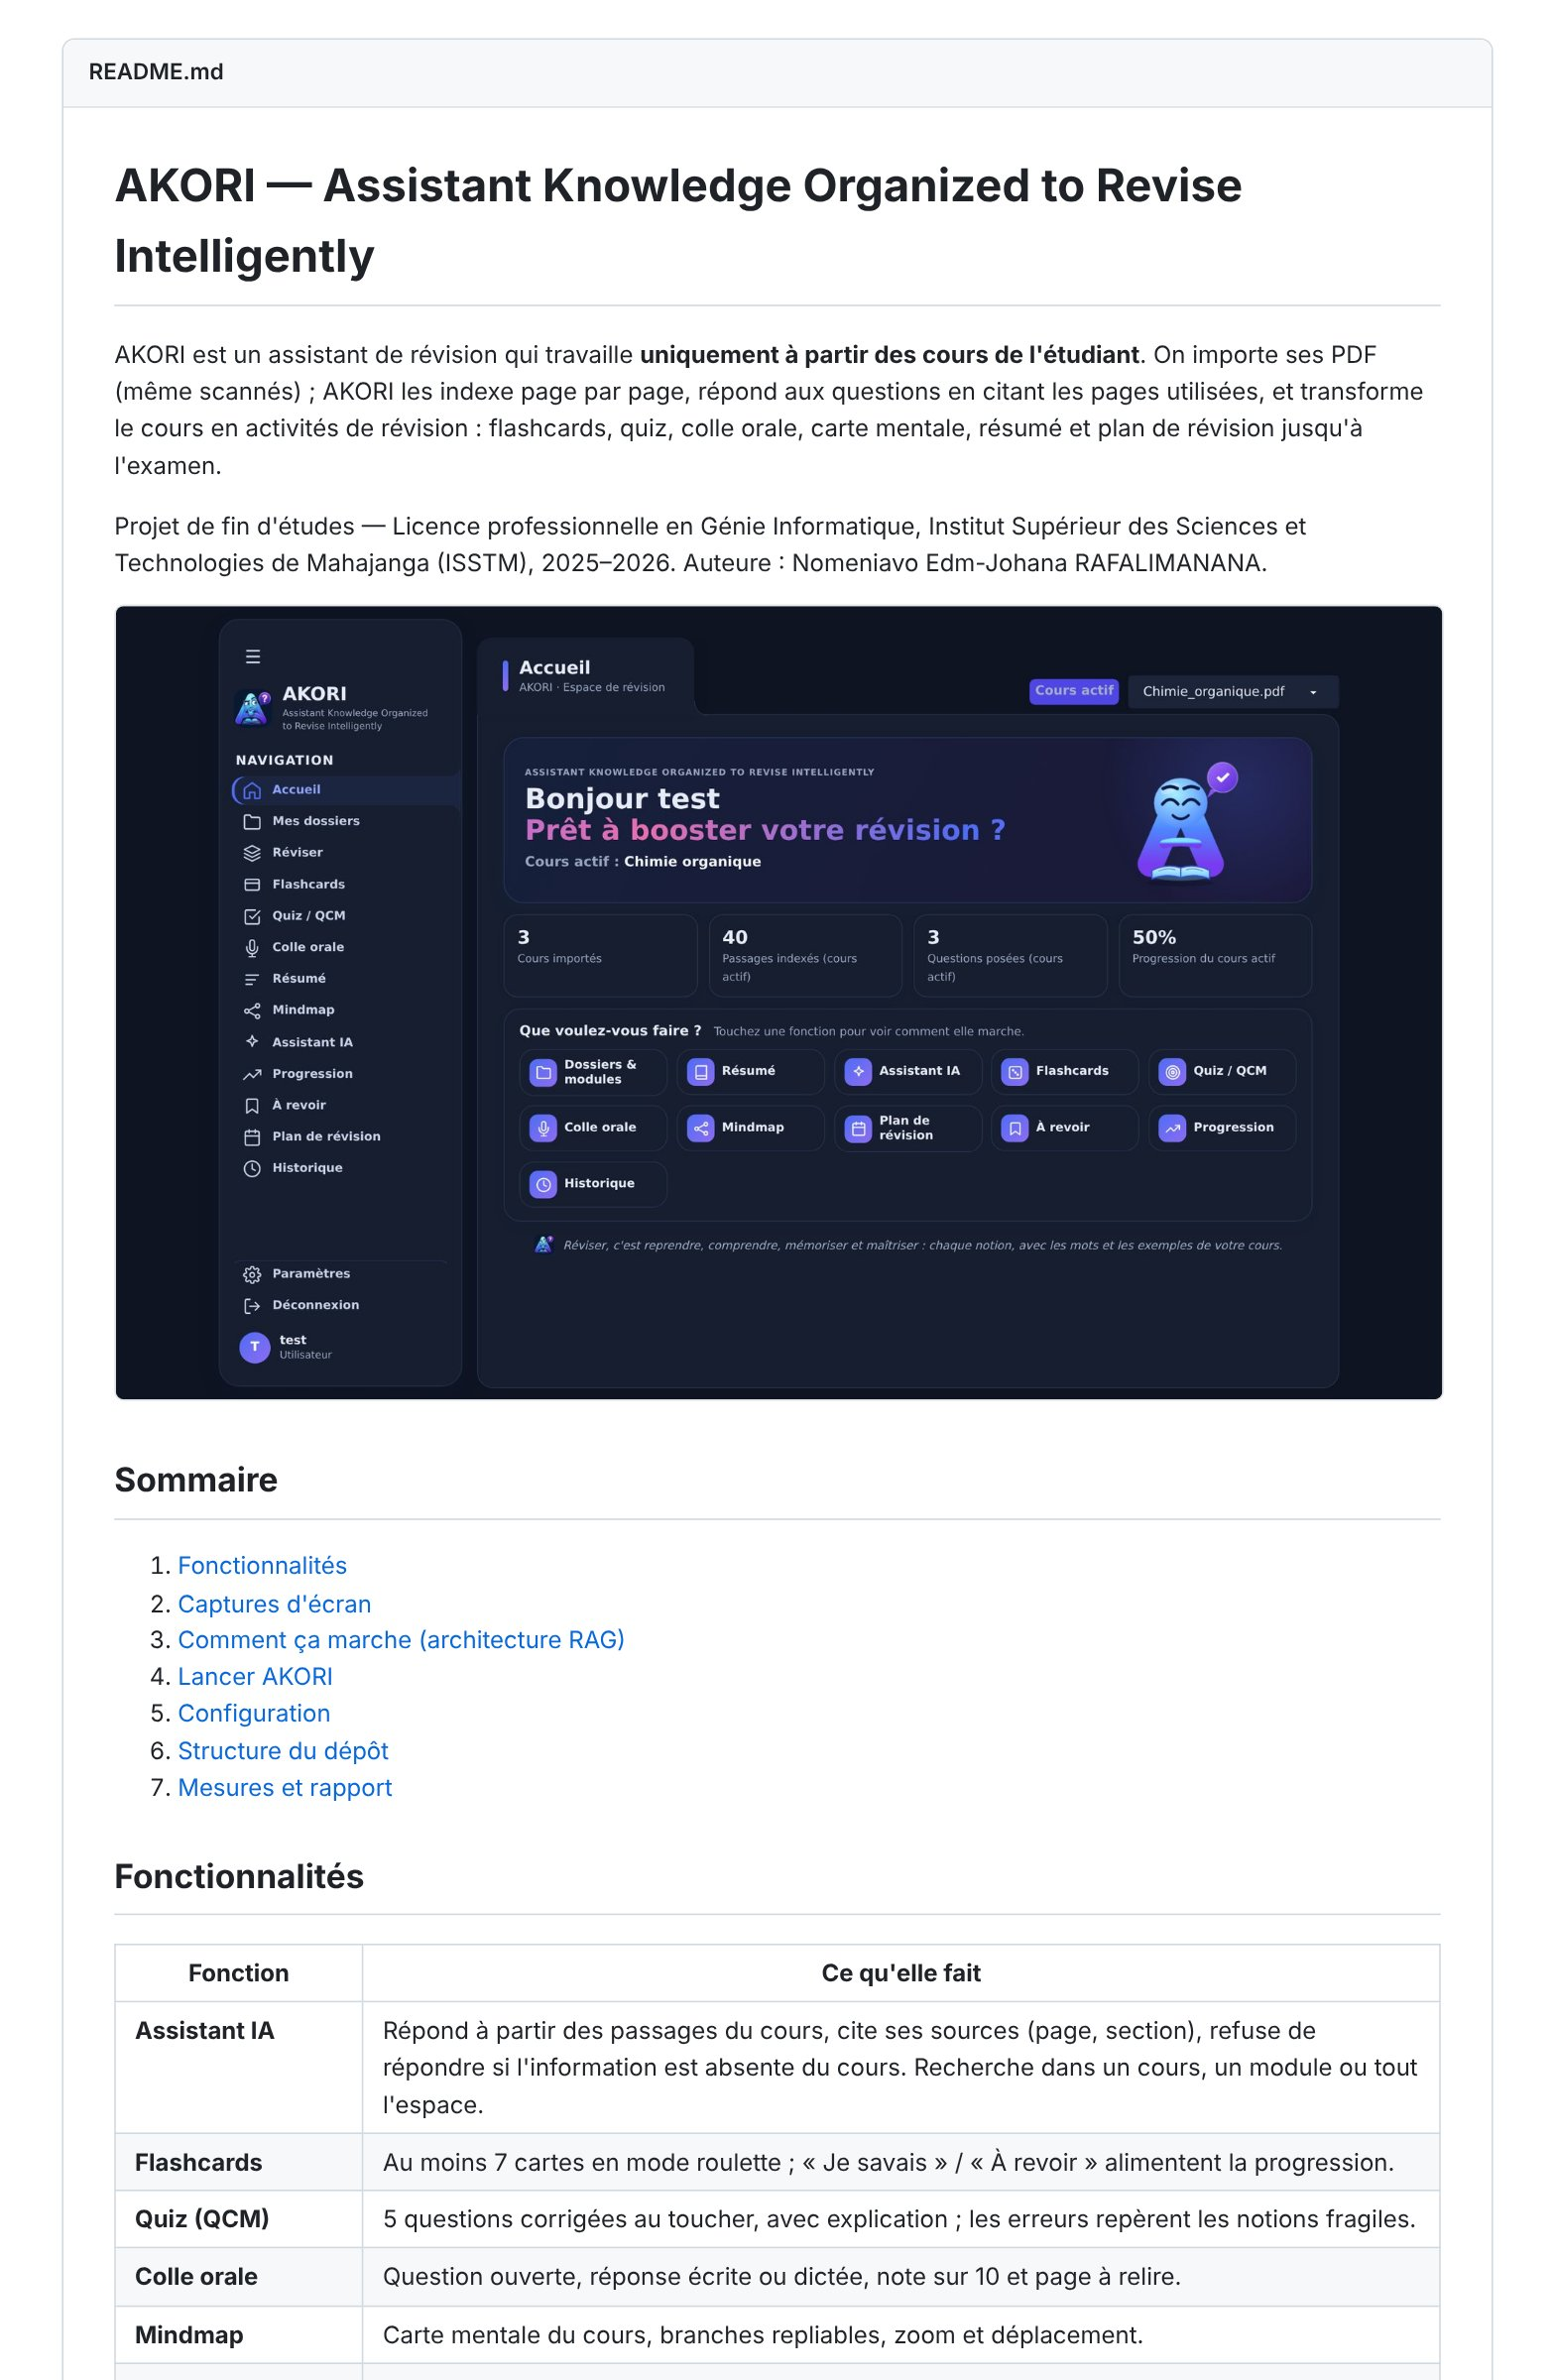
\includegraphics[width=0.78\textwidth]{images/annexe/09_readme_depot.jpg}
  \caption{Début du README du dépôt : présentation, capture de l'interface et fonctionnalités}
  \label{fig:readme}
\end{figure}

\chapter{Captures d'écran de l'interface}\label{annexe:captures}

Les captures suivantes ont été réalisées sur la version finale d'AKORI, avec un compte et des cours de démonstration.

\begin{figure}[H]
  \centering
  
\includegraphics[width=0.92\textwidth]{images/annexe/00_presentation.jpg}
  \caption{Page de présentation affichée avant la connexion}
\end{figure}

\begin{figure}[H]
  \centering
  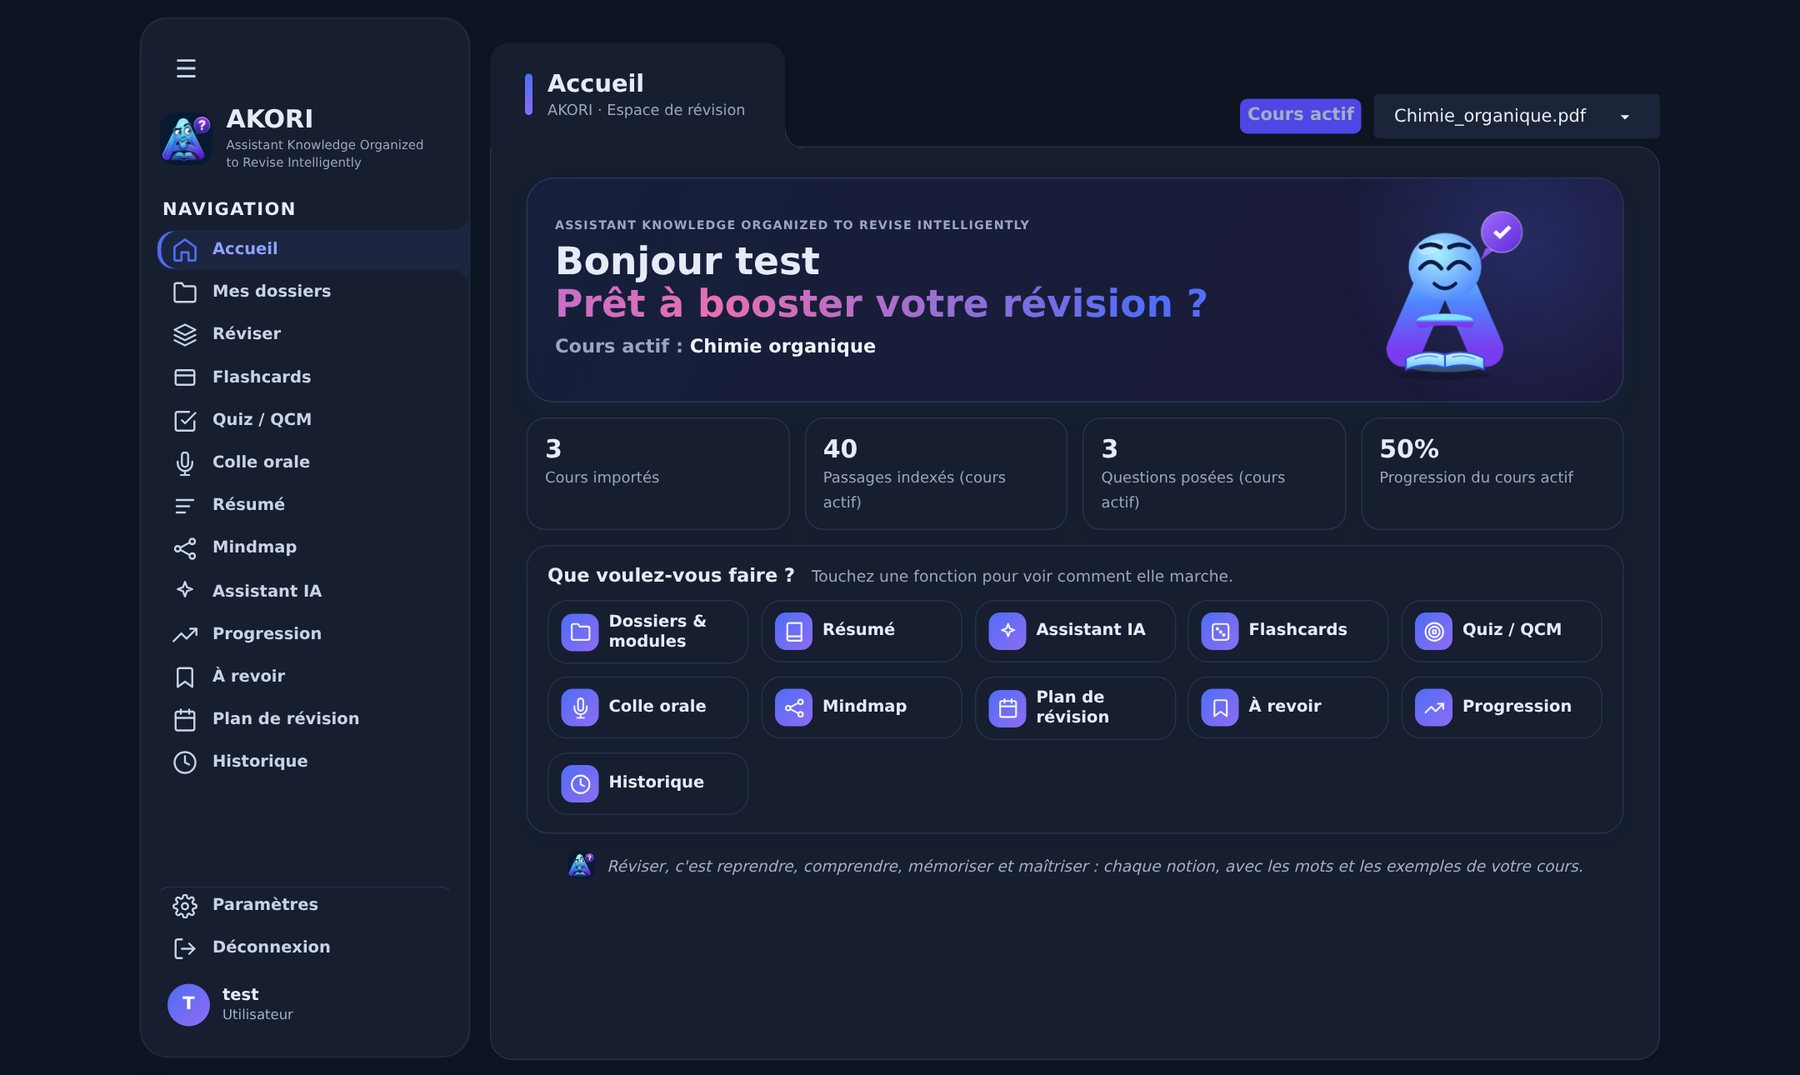
\includegraphics[width=0.92\textwidth]{images/annexe/01_accueil.jpg}
  \caption{Accueil (thème sombre) : indicateurs du cours actif et accès aux fonctions}
\end{figure}

\begin{figure}[H]
  \centering
  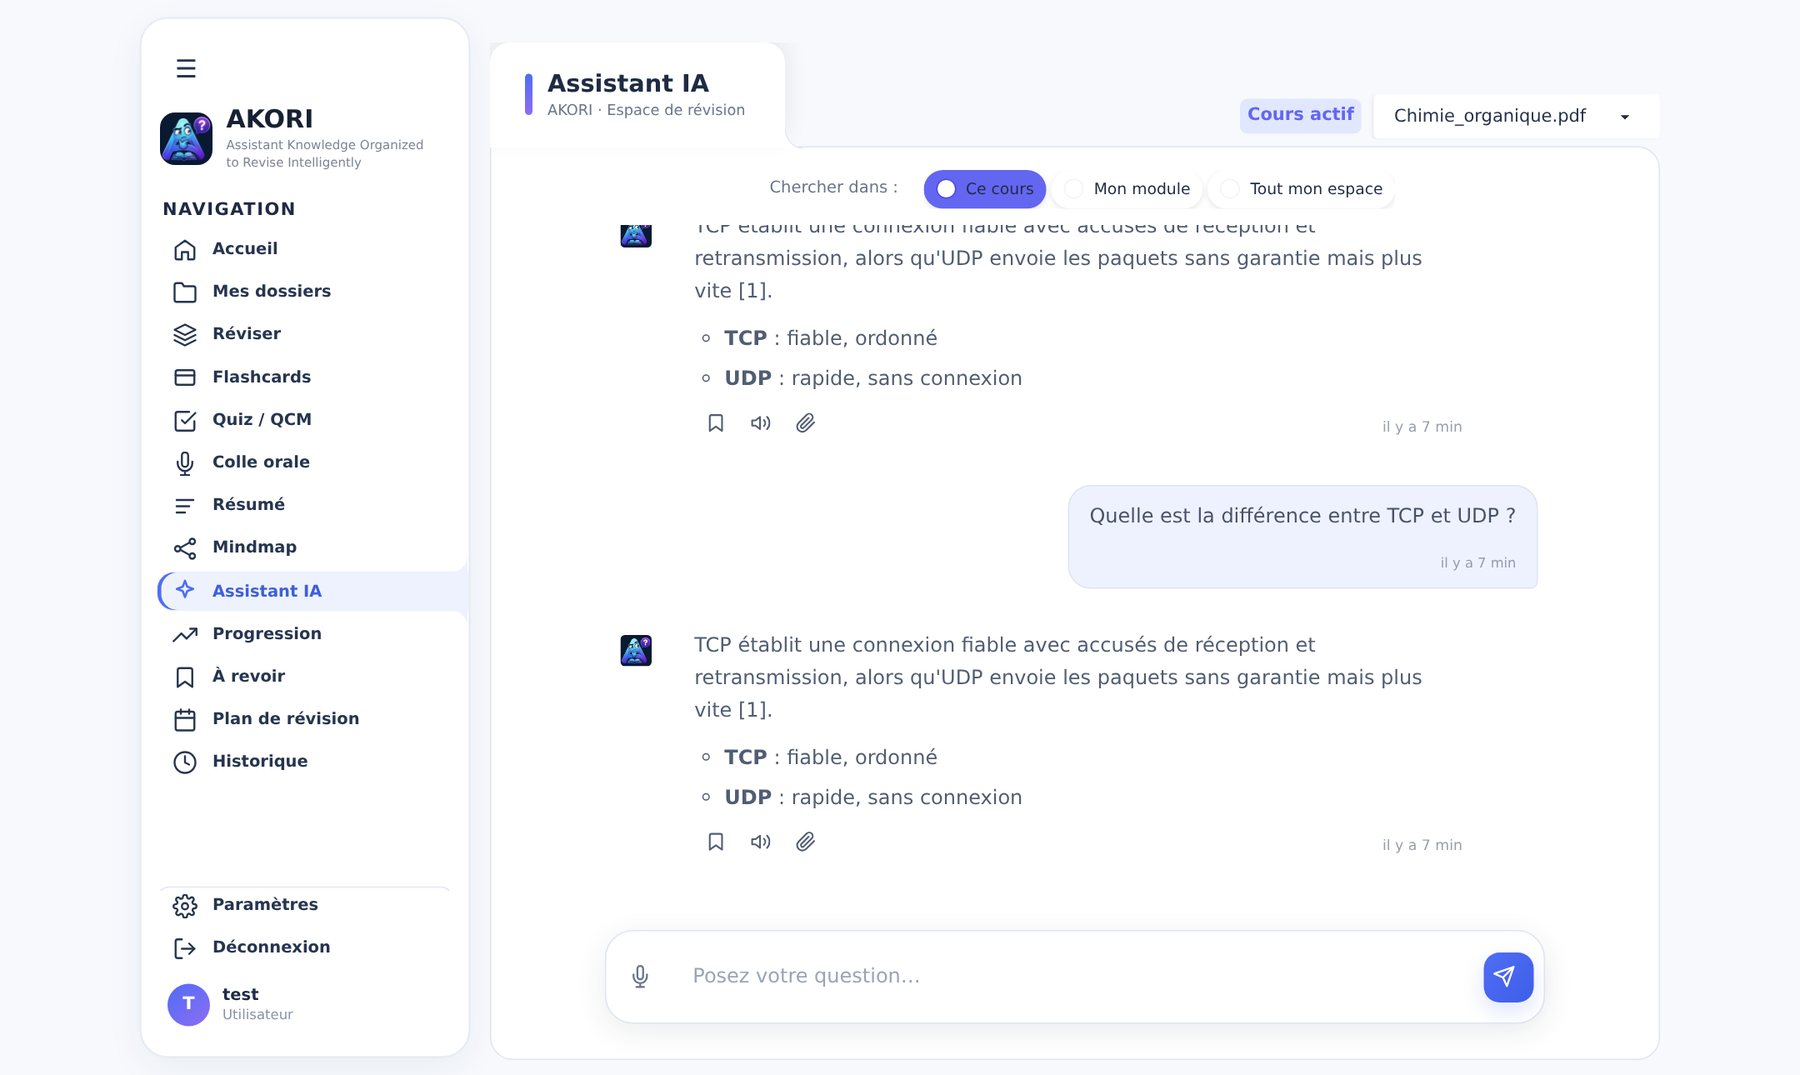
\includegraphics[width=0.92\textwidth]{images/annexe/02_assistant.jpg}
  \caption{Assistant IA : réponse rédigée à partir du cours, avec ses sources}
\end{figure}

\begin{figure}[H]
  \centering
  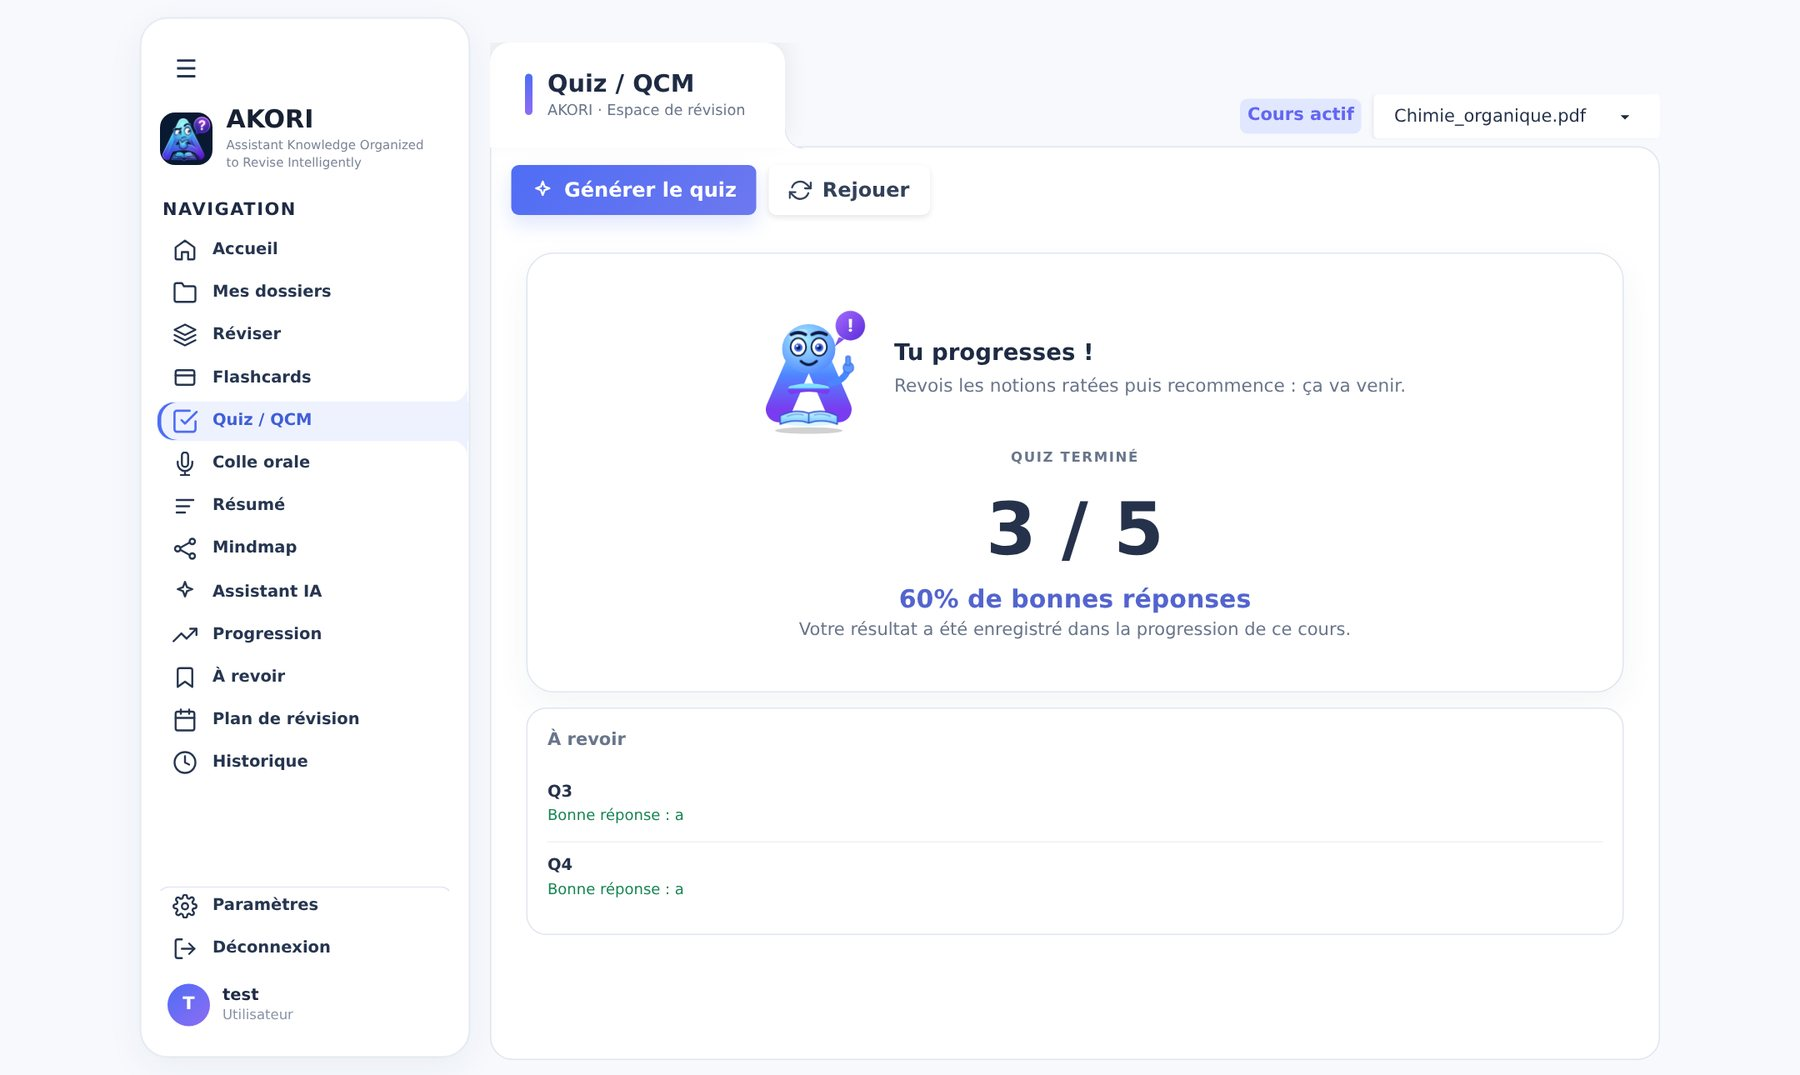
\includegraphics[width=0.92\textwidth]{images/annexe/03_quiz_resultat.jpg}
  \caption{Quiz (QCM) corrigé à partir du cours}
\end{figure}

\begin{figure}[H]
  \centering
  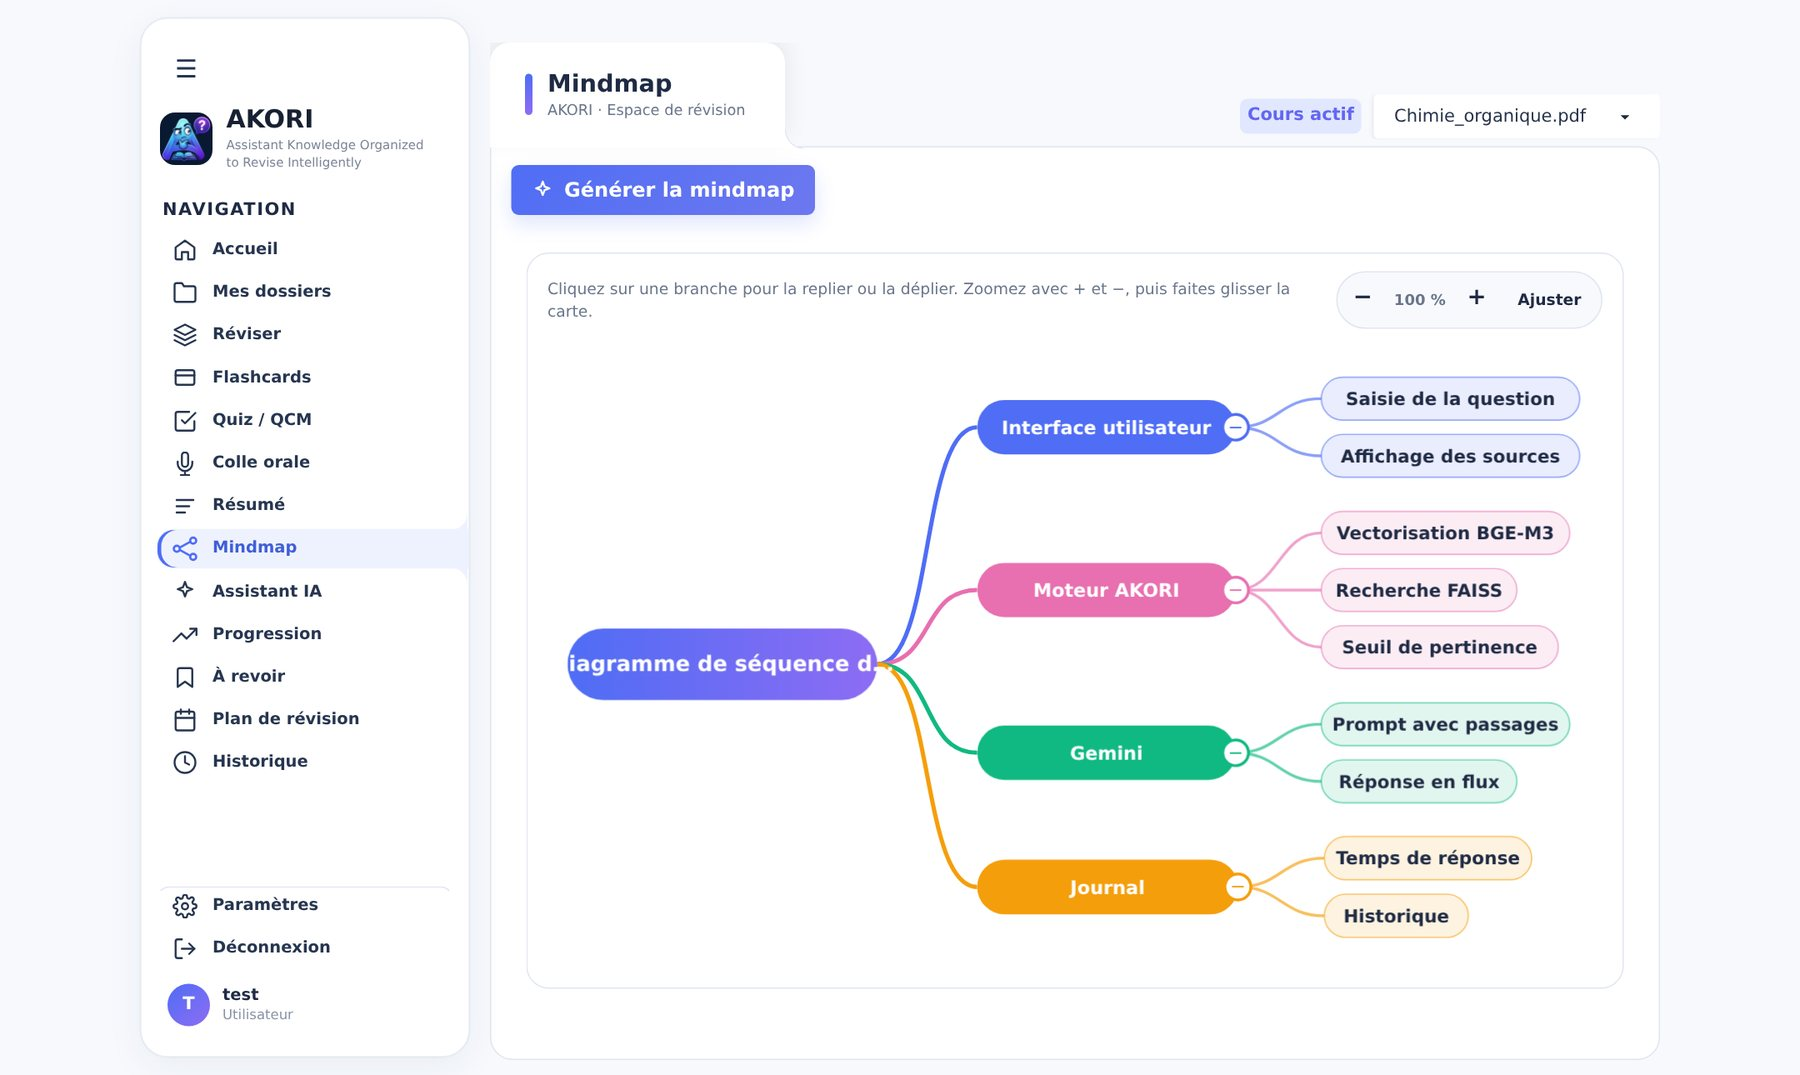
\includegraphics[width=0.92\textwidth]{images/annexe/04_mindmap.jpg}
  \caption{Mindmap du cours, avec zoom et déplacement}
\end{figure}

\begin{figure}[H]
  \centering
  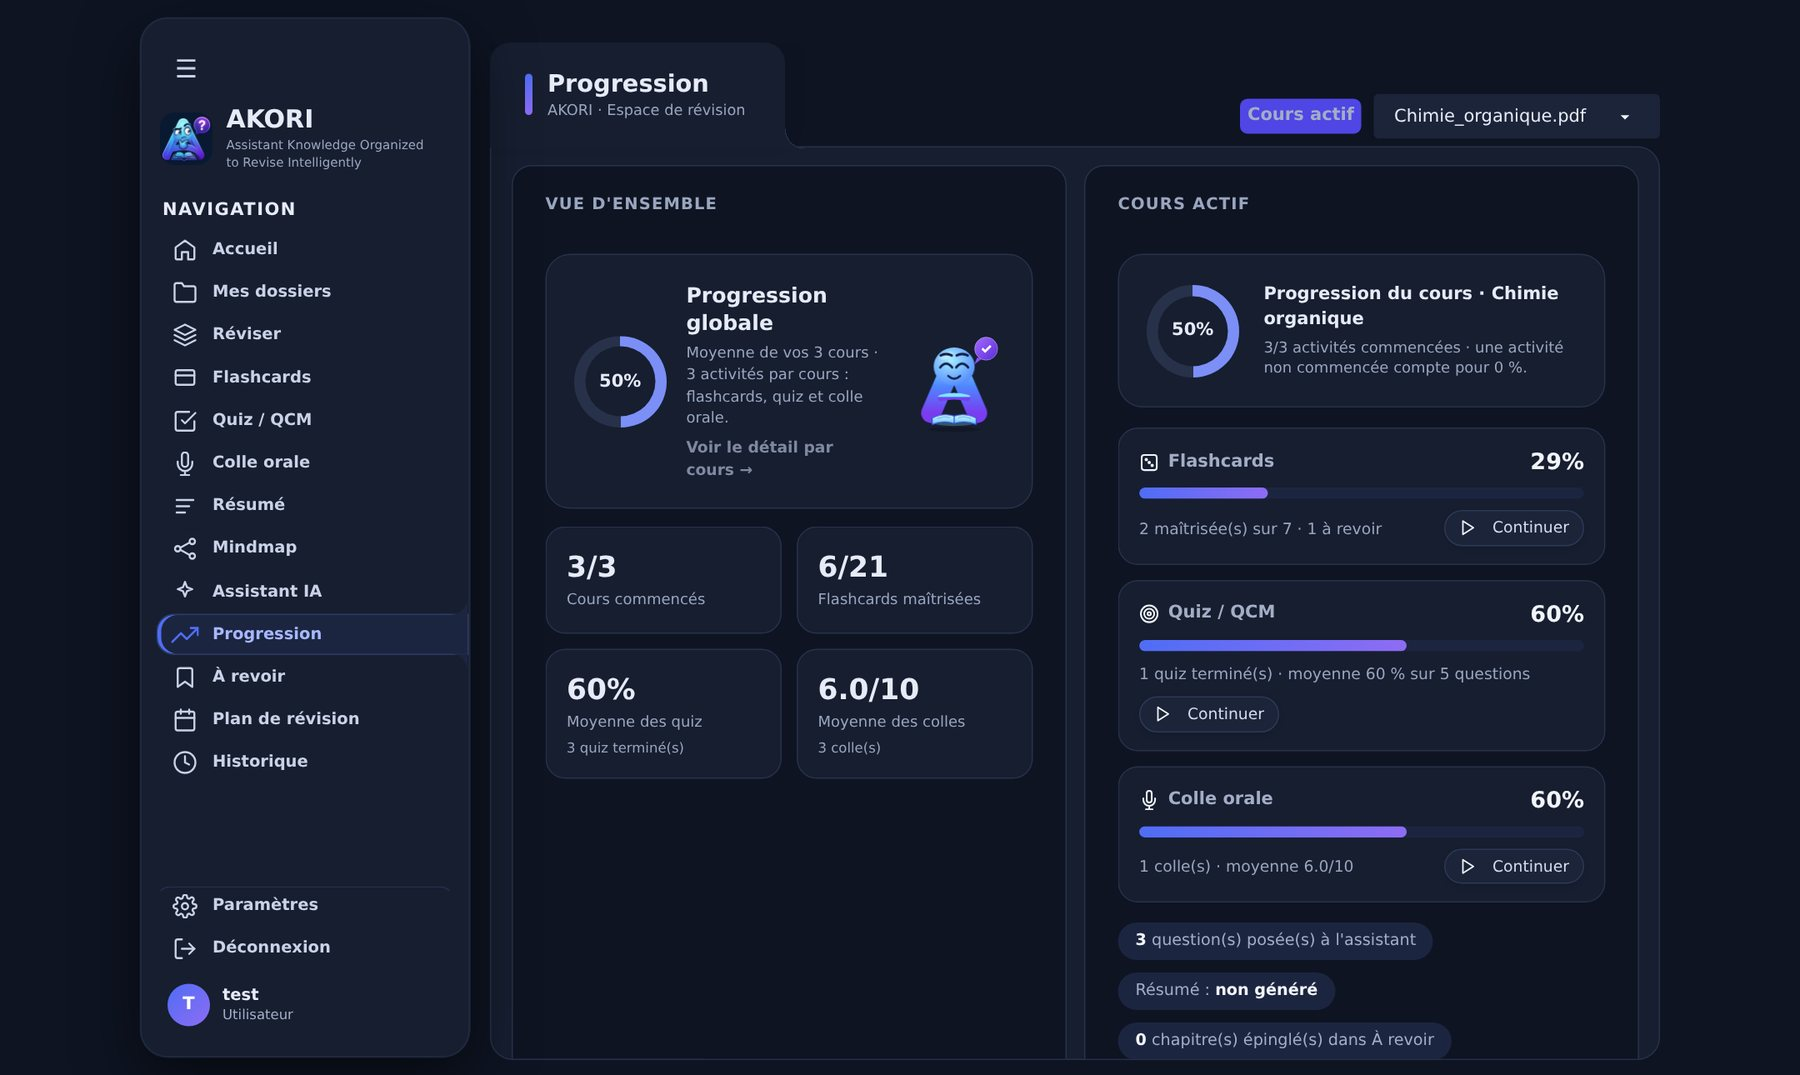
\includegraphics[width=0.92\textwidth]{images/annexe/05_progression.jpg}
  \caption{Progression par cours (flashcards, quiz, colle orale)}
\end{figure}

\begin{figure}[H]
  \centering
  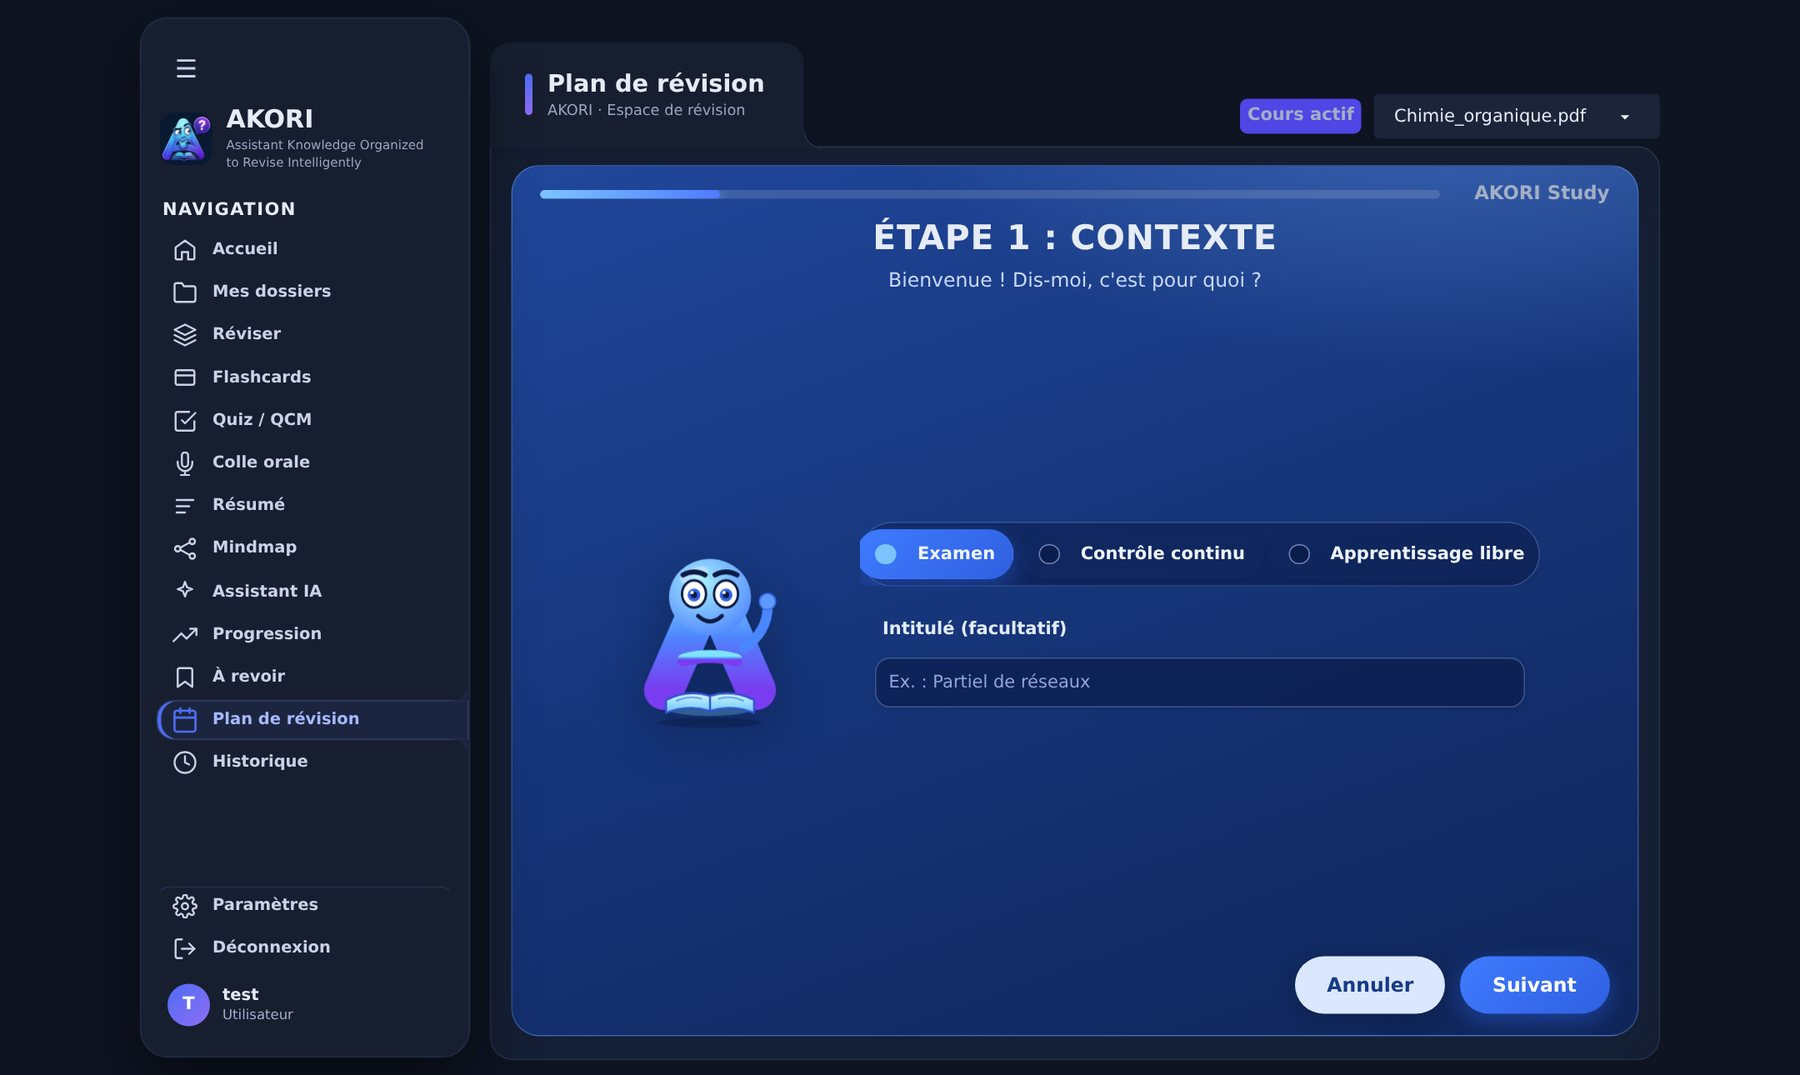
\includegraphics[width=0.92\textwidth]{images/annexe/06_plan_assistant.jpg}
  \caption{Plan de révision : assistant en cinq étapes}
\end{figure}

\begin{figure}[H]
  \centering
  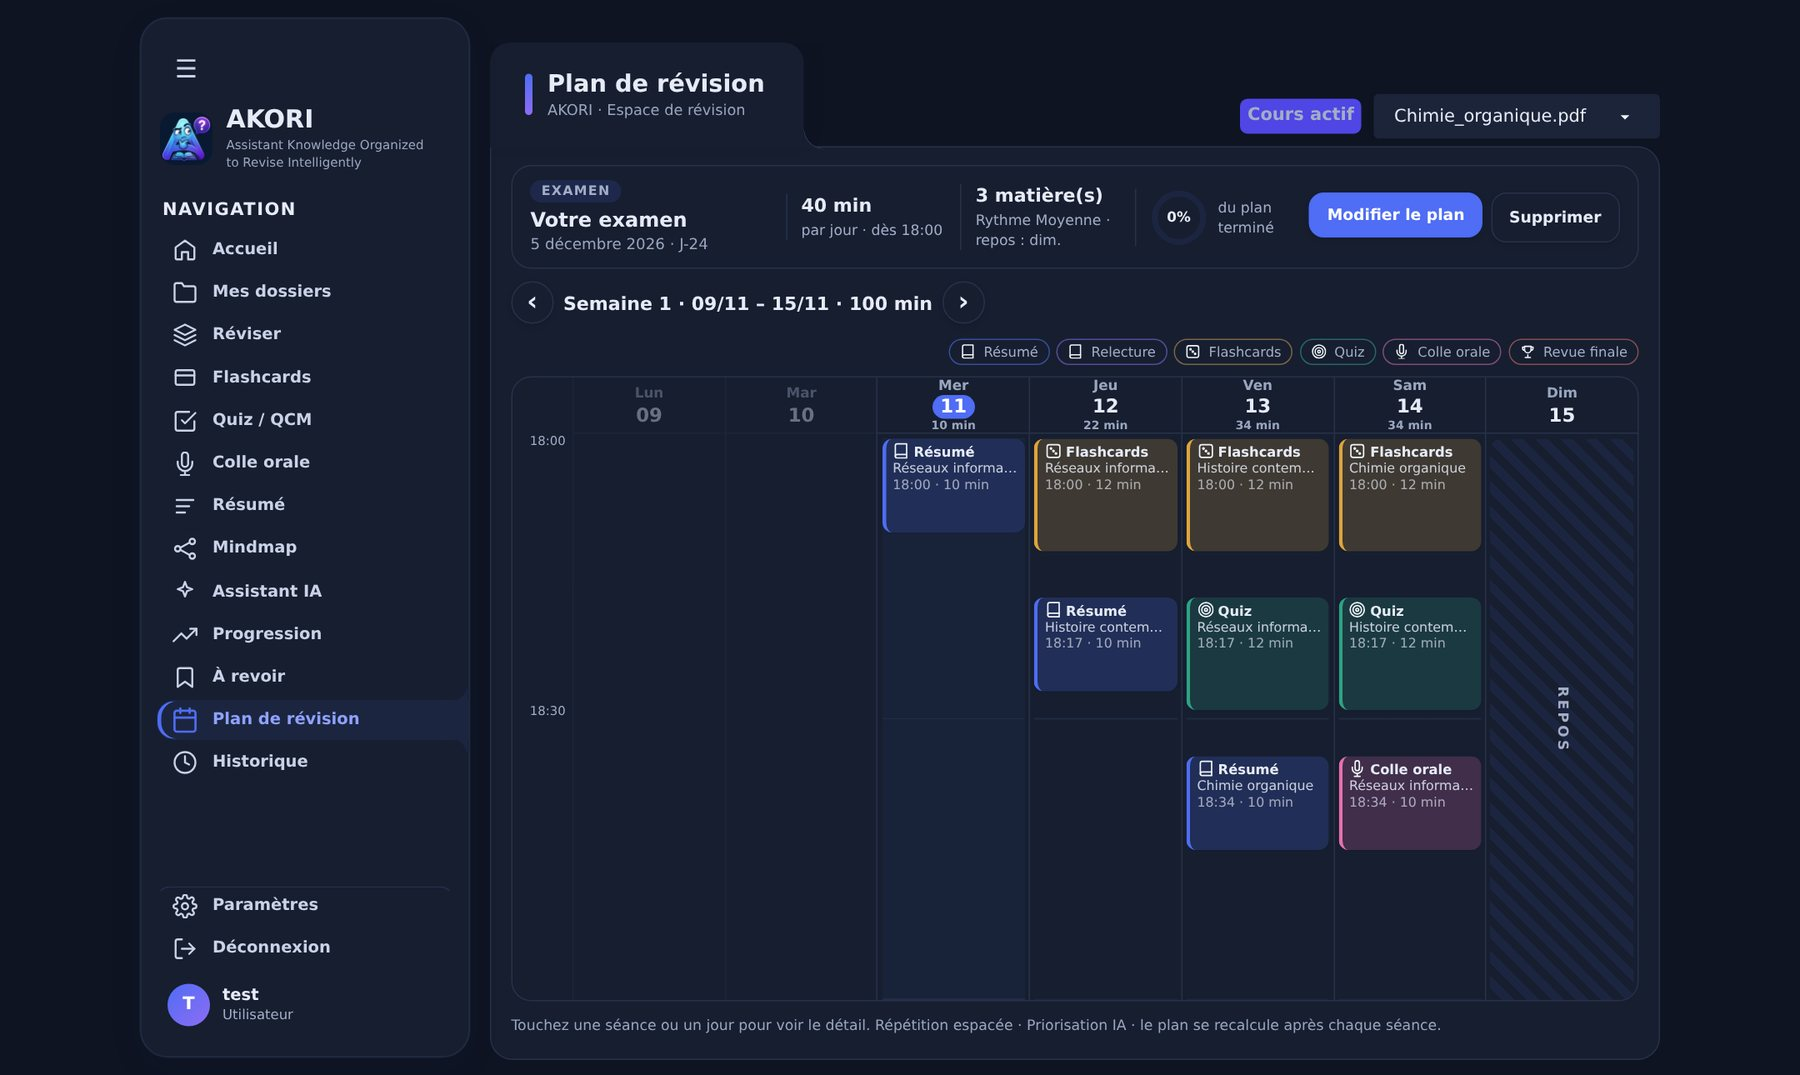
\includegraphics[width=0.92\textwidth]{images/annexe/07_plan_emploi_du_temps.jpg}
  \caption{Plan de révision : emploi du temps généré, cliquable pour le détail de chaque séance}
\end{figure}

\begin{figure}[H]
  \centering
  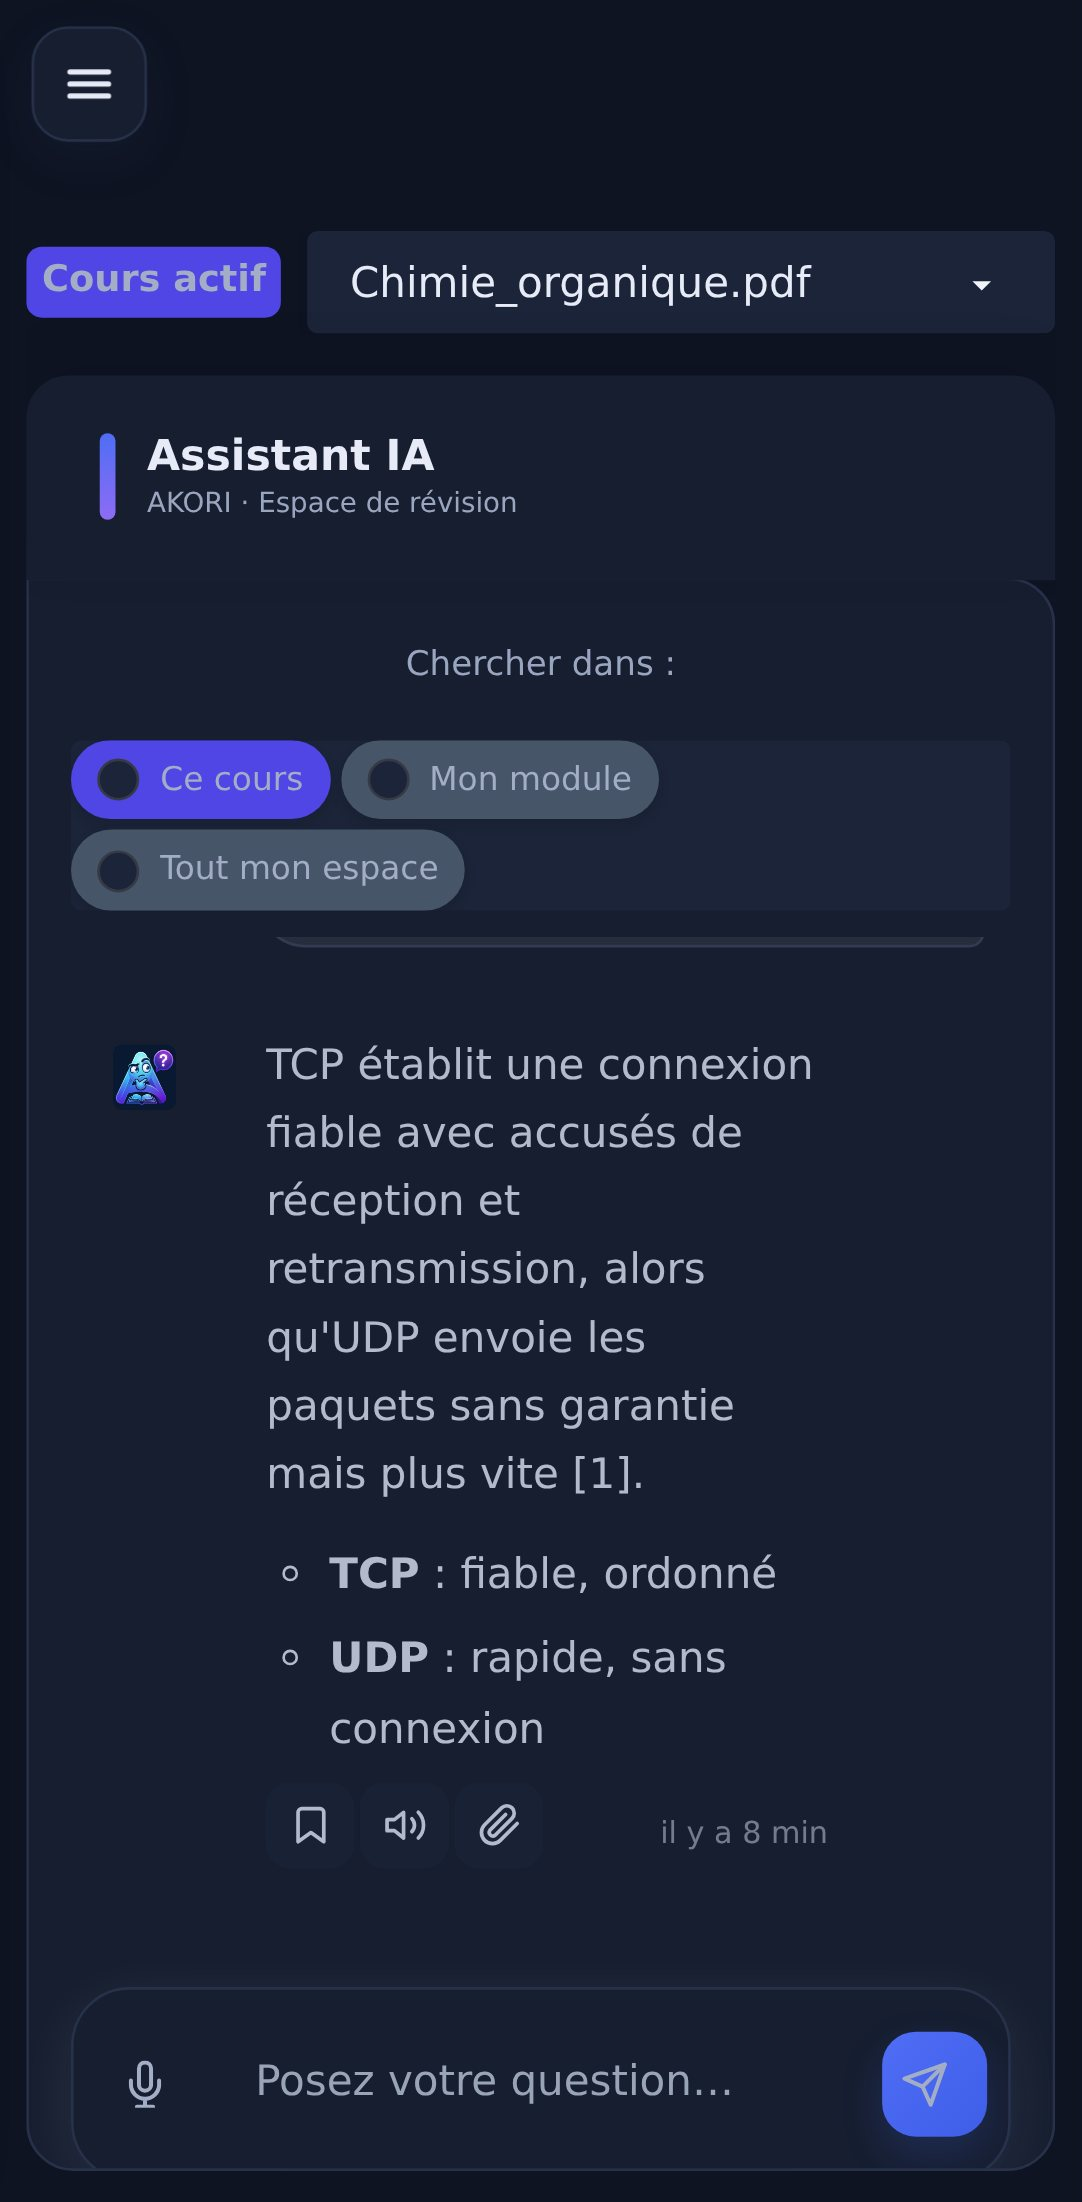
\includegraphics[height=0.62\textheight,keepaspectratio]{images/annexe/08_telephone_assistant.jpg}
  \caption{Version téléphone : assistant IA}
\end{figure}

\chapter{Protocole et résultats détaillés des tests}\label{annexe:tests}

\section{Environnement et cours de test}

\begin{itemize}[nosep]
  \item \textbf{Date des mesures} : \BenchDate.
  \item \textbf{Machine} : conteneur Linux, \BenchCPU{} processeurs virtuels, \BenchMateriel.
  \item \textbf{Réglages d'AKORI} : réglages par défaut (BGE-M3, fragments de 800 caractères avec 80 de chevauchement, $k = 4$, seuil 0,30, OCR Tesseract).
  \item \textbf{Cours de test} : ce rapport au format PDF (\IdxPages{} pages, \IdxFragments{} fragments). Les \OcrPages{} premières pages ont aussi été converties en images sans texte pour mesurer l'OCR.
\end{itemize}

\section{Séries de questions et critères}

\begin{itemize}
  \item \textbf{Dans le cours} (\SeuilCoursN{} questions) et \textbf{reformulées} (\SeuilRefoN{} questions, mêmes notions avec d'autres mots) : chaque question est associée à un ou plusieurs éléments de réponse attendus (par exemple « 800 », « PBKDF2 »). Un passage est jugé pertinent s'il contient l'un d'eux.
  \item \textbf{Proches du sujet, réponse absente} (\SeuilAbsN{} questions) : questions sur AKORI dont la réponse ne figure nulle part dans le cours ; l'absence a été vérifiée dans le texte du PDF.
  \item \textbf{Hors sujet} (\SeuilHorsN{} questions) : culture générale, sciences, cuisine, sport, etc.
\end{itemize}

Pour chaque question, le banc relève la similarité cosinus du meilleur passage (« Sim. max »), la présence d'un passage pertinent parmi les quatre retenus (« Passage »), la décision du seuil et, si l'API Gemini est accessible, la réponse finale : « juste » lorsque l'élément attendu y figure, « refus » lorsque AKORI indique que l'information ne figure pas dans le cours.

\clearpage
\section{Résultats question par question}

{\small
% Fichier généré par rapport/benchmark_akori.py : ne pas modifier à la main.
\begin{longtable}{@{}r p{0.50\textwidth} c c c c@{}}
\caption{Résultat de chaque question du banc de test.}\label{tab:questions}\\
\toprule \# & Question & Sim. max & Passage & Seuil & Réponse \\ \midrule \endfirsthead
\toprule \# & Question & Sim. max & Passage & Seuil & Réponse \\ \midrule \endhead
\bottomrule \endfoot
\multicolumn{6}{@{}l}{\textbf{Dans le cours}} \\
1 & Quel modèle d'embedding utilise AKORI ? & 0{,}68 & oui & accepté & \nonmesure \\
2 & Quelle bibliothèque assure la recherche vectorielle des passages ? & 0{,}57 & oui & accepté & \nonmesure \\
3 & Quelle est la taille des fragments lors du découpage du texte ? & 0{,}70 & oui & accepté & \nonmesure \\
4 & Quel chevauchement est conservé entre deux fragments successifs ? & 0{,}65 & oui & accepté & \nonmesure \\
5 & Combien de passages sont transmis au modèle génératif pour une question ? & 0{,}63 & oui & accepté & \nonmesure \\
6 & Quel est le seuil de pertinence utilisé par défaut ? & 0{,}57 & oui & accepté & \nonmesure \\
7 & Quel modèle génératif principal est utilisé par AKORI ? & 0{,}63 & non & accepté & \nonmesure \\
8 & Quelle méthode protège les mots de passe des comptes ? & 0{,}60 & oui & accepté & \nonmesure \\
9 & Combien d'itérations utilise la dérivation des mots de passe ? & 0{,}57 & oui & accepté & \nonmesure \\
10 & Quelle bibliothèque extrait le texte des fichiers PDF ? & 0{,}57 & oui & accepté & \nonmesure \\
11 & Quel moteur OCR lit les pages scannées ? & 0{,}59 & oui & accepté & \nonmesure \\
12 & Avec quel outil l'interface web a-t-elle été construite ? & 0{,}56 & oui & accepté & \nonmesure \\
13 & Quel modèle de langage local a été testé au début du projet ? & 0{,}54 & oui & accepté & \nonmesure \\
14 & Quelle latence observait le prototype exécuté localement ? & 0{,}61 & oui & accepté & \nonmesure \\
15 & Quels sont les intervalles de la répétition espacée du plan de révision ? & 0{,}64 & oui & accepté & \nonmesure \\
16 & Quelle est la dimension des vecteurs produits par BGE-M3 ? & 0{,}66 & oui & accepté & \nonmesure \\
17 & Que signifie le sigle RAG ? & 0{,}54 & oui & accepté & \nonmesure \\
18 & Sur combien de points la colle orale est-elle notée ? & 0{,}59 & oui & accepté & \nonmesure \\
19 & Où sont enregistrées les données lorsque l'application tourne sur Colab ? & 0{,}59 & oui & accepté & \nonmesure \\
\midrule
\multicolumn{6}{@{}l}{\textbf{Reformulées}} \\
20 & Quel outil compare les vecteurs pour retrouver les extraits les plus proches ? & 0{,}58 & oui & accepté & \nonmesure \\
21 & Avec quel modèle les textes sont-ils transformés en listes de nombres ? & 0{,}57 & oui & accepté & \nonmesure \\
22 & Comment l'application lit-elle les pages qui ne sont que des images ? & 0{,}64 & oui & accepté & \nonmesure \\
23 & Que fait l'assistant quand aucun extrait n'est assez proche de la demande ? & 0{,}55 & non & accepté & \nonmesure \\
24 & Pourquoi a-t-on renoncé à faire tourner le modèle de langage sur la machine ? & 0{,}49 & oui & accepté & \nonmesure \\
25 & Comment les secrets de connexion des utilisateurs sont-ils conservés de façon sûre ? & 0{,}58 & oui & accepté & \nonmesure \\
26 & Quelle est la longueur de chaque morceau de texte indexé ? & 0{,}59 & oui & accepté & \nonmesure \\
27 & Sur quel principe de psychologie reposent les cartes mémoire et les questionnaires ? & 0{,}51 & non & accepté & \nonmesure \\
28 & Comment l'application continue-t-elle de répondre quand le service d'IA est saturé ? & 0{,}54 & non & accepté & \nonmesure \\
29 & Où peut-on héberger l'application pour qu'elle ait une adresse permanente ? & 0{,}56 & oui & accepté & \nonmesure \\
\midrule
\multicolumn{6}{@{}l}{\textbf{Proches du sujet, réponse absente du cours}} \\
30 & Quelle est la taille maximale d'un PDF importé ? & 0{,}62 & -- & accepté & \nonmesure \\
31 & Combien coûte un abonnement mensuel à AKORI ? & 0{,}59 & -- & accepté & \nonmesure \\
32 & Quelle version de Python est utilisée dans l'image Docker ? & 0{,}55 & -- & accepté & \nonmesure \\
33 & Sur quel port réseau l'application écoute-t-elle sur le serveur ? & 0{,}53 & -- & accepté & \nonmesure \\
34 & Combien d'étudiants ont testé AKORI pendant le semestre ? & 0{,}62 & -- & accepté & \nonmesure \\
35 & AKORI fonctionne-t-il sur un Raspberry Pi ? & 0{,}64 & -- & accepté & \nonmesure \\
\midrule
\multicolumn{6}{@{}l}{\textbf{Hors sujet}} \\
36 & Quelle est la capitale de l'Australie ? & 0{,}30 & -- & refus & \nonmesure \\
37 & Comment fonctionne la photosynthèse chez les plantes ? & 0{,}43 & -- & accepté & \nonmesure \\
38 & Qui a peint le tableau de la Joconde ? & 0{,}28 & -- & refus & \nonmesure \\
39 & Quelle est la formule de l'aire d'un cercle ? & 0{,}39 & -- & accepté & \nonmesure \\
40 & Expliquez la théorie de la relativité restreinte d'Einstein. & 0{,}44 & -- & accepté & \nonmesure \\
41 & Comment préparer une pâte à crêpes ? & 0{,}41 & -- & accepté & \nonmesure \\
42 & Quelles sont les causes de la Première Guerre mondiale ? & 0{,}36 & -- & accepté & \nonmesure \\
43 & Quel est le rôle des mitochondries dans la cellule ? & 0{,}41 & -- & accepté & \nonmesure \\
44 & Comment calculer la dérivée d'une fonction polynomiale ? & 0{,}41 & -- & accepté & \nonmesure \\
45 & Qu'est-ce que le protocole de routage OSPF ? & 0{,}44 & -- & accepté & \nonmesure \\
46 & Quel est le plus long fleuve d'Afrique ? & 0{,}33 & -- & accepté & \nonmesure \\
47 & Comment fonctionne un moteur à explosion ? & 0{,}45 & -- & accepté & \nonmesure \\
48 & Quelles sont les règles du hors-jeu au football ? & 0{,}37 & -- & accepté & \nonmesure \\
49 & Qu'est-ce que l'inflation en économie ? & 0{,}42 & -- & accepté & \nonmesure \\
50 & Comment soigner une grippe saisonnière ? & 0{,}35 & -- & accepté & \nonmesure \\
51 & Quelle est la vitesse de la lumière dans le vide ? & 0{,}41 & -- & accepté & \nonmesure \\
52 & Qui a écrit le roman Les Misérables ? & 0{,}30 & -- & refus & \nonmesure \\
53 & Comment fonctionne la blockchain du Bitcoin ? & 0{,}46 & -- & accepté & \nonmesure \\
54 & Quelles sont les étapes de la mitose ? & 0{,}42 & -- & accepté & \nonmesure \\
55 & Comment se forme un arc-en-ciel ? & 0{,}41 & -- & accepté & \nonmesure \\
\end{longtable}

}

\section{Reproduire les mesures}

Toutes les valeurs chiffrées du chapitre~\ref{chap:resultats} et de cette annexe proviennent des fichiers générés par le banc de test ; elles se mettent à jour à chaque compilation.

\begin{itemize}
  \item Mesure complète (indexation, OCR, recherche, seuil et réponses) : \\
  \texttt{python rapport/benchmark\_akori.py rapport.pdf -{}-gemini -{}-ocr-pages 10}
  \item Réponses de Gemini seulement, en gardant les autres mesures : \\
  \texttt{python rapport/benchmark\_akori.py rapport.pdf -{}-seulement gemini}
  \item Régénérer les tableaux LaTeX à partir des résultats : \\
  \texttt{python rapport/benchmark\_akori.py -{}-tex}
\end{itemize}

Le banc écrit \texttt{rapport/resultats\_benchmark.json} (toutes les mesures, y compris le texte des réponses) ainsi que \texttt{resultats\_benchmark.tex}, \texttt{resultats\_questions.tex} et \texttt{resultats\_balayage.tex}, lus par ce rapport.

\end{document}
